\documentclass[english, a4paper, 11pt, twoside, numbers=noenddot, openright,version=3.21]{scrbook}

% Page layout
\usepackage{geometry}                    % set page layout
\usepackage{setspace}                    % set line spacing
\usepackage[automark]{scrlayer-scrpage}  % Koma header and footer package

% Language, coding and font
\usepackage{lmodern}                     % Font - as requested by ILS
\usepackage[english]{babel}              % Language setting (last defined is standard)
\usepackage[T1]{fontenc}                 % Hyphenation for words with Umlaute
\usepackage[utf8]{inputenc}              % Coding for correct display of Umlaute
\usepackage[english]{translator}         % Übersetzer
\usepackage{longtable}                   % Tables with page break
\usepackage{tabu}                        % Advanced table package
\usepackage{datetime}                    % Date and time formatting
\usepackage{ltablex}                     % Use this package instead of tabularx for long tables with X columns

% Graphics and colors
\usepackage[pdftex]{graphicx}            % Include graphics
\usepackage{epstopdf}                    % Include eps graphics
\usepackage{color}                       % Colors
\usepackage{xcolor}                      % Advanced colors
\usepackage{listings}                    % Code listings


\usepackage{pythonhighlight}             % Highlight Python code
\usepackage{wrapfig}                     % Wrap images in text
\usepackage{framed}                      % Gray background for quotes

% Math
\usepackage{amsmath,amsthm}              % Math environment
\usepackage{textcomp}                     % Degree symbol

% Floats
\usepackage[section]{placeins}           % Control float placement, \FloatBarrier command

% Other
\usepackage[hyphens]{url}                % URL
\usepackage{hyperref}                    % Settings for PDF document
\usepackage{caption}                     % for modification caption format
\captionsetup{format=plain}              % This removes the indentation
\usepackage{subcaption}                  % For subfigures
\usepackage{csquotes}                    % Recommended
\usepackage{pdfpages}                    % include PDF pages
\usepackage{lipsum}                      % lorem ipsum blindtext
\usepackage{siunitx}                     % si einheiten
\usepackage{microtype}                   % underfull und overfull box problem minimierung
\usepackage{etoolbox}                    % Appendix Buchstabenseitenzahl
\usepackage{float}                       % In der Lage figures explizit an einer Stelle im Text zu fixieren
\setuptoc{toc}{totoc}                    % Add table of contents to the table of contents
\setuptoc{lof}{totoc}                    % Add list of figures to the table of contents
\setuptoc{lot}{totoc}                    % Add list of tables to the table of contents
\setuptoc{bib}{totoc}                    % Add bibliography to the table of contents
\usepackage{ulem}                        % Underline text
\usepackage{paralist}                    % Modifikation von Listen
\usepackage{titling}                     % \theauthor macro
\usepackage{tabularx}                    % Tabellen
\usepackage{ragged2e}                    % Textausrichtung

% Customizable Enumerates/Itemizes
\usepackage{enumitem}                    % Bsp.: Option "style=nextline" für eine gleichmäßige Einrückung aller Zeilen

% Tables
\usepackage{lscape}                      % mehrseitige Tabellen
\usepackage{booktabs}                    % \toprule \midrule \bottomrule
\usepackage{colortbl}                    % farbige Tabellen / Tabellen einfärben
\usepackage{multirow}                    % mehrere Zeilen verbinden
\usepackage{array}                       % Hilfsmittel zum Setzen von Tabellen und geordneten Texten im Mathematischem Modus

% Bibliography
\usepackage[
    backend=bibtex,                      % Backends Biblatex
    style=ieee,                          % Bibliogragrafiestil IEEE
    natbib=true                          % Kompatibilitätsmodul natbib
]{biblatex}
\addbibresource{./bibliography/bib.bib}  % Dateipfad zur Bib Datei

% Glossaries
\usepackage[
    xindy,
    nonumberlist,                        % keine Seitenzahlen anzeigen
    nopostdot,                           % keine Punkte
    style=super,                         % Style
    acronym,                             % ein Abkkürzungsverzeichnis erstellen
    toc,                                 % Einträge im Inhaltsverzeichnis
    section=chapter                      % im Inhaltsverzeichnis auf section-Ebene erscheinen
]{glossaries}
\geometry{% 									
left = 2.5cm, 
right=2.5cm, 
top=1.4cm, 
bottom=1.1cm,
includeheadfoot,								
headsep = \dimexpr2\baselineskip-3mm\relax,		% Abstand der Kopfzeile zum Kontext
footskip = \dimexpr2\baselineskip+4mm\relax,	% Abstand der Fußzeile zum Kontext
bindingoffset=1.5mm, 							% max. halb so groß wie der Buchrücken
%showframe										% Rahmen einblenden
}
\KOMAoptions{parskip=yes}						% keine Einrückungen

\makeatletter
\newcommand{\MSonehalfspacing}{%
	\setstretch{1.44}%  default
	\ifcase \@ptsize \relax % 10pt
	\setstretch {1.448}%
	\or % 11pt
	\setstretch {1.399}%
	\or % 12pt
	\setstretch {1.433}%
	\fi
}
\newcommand{\MSdoublespacing}{%
	\setstretch {1.92}%  default
	\ifcase \@ptsize \relax % 10pt
	\setstretch {1.936}%
	\or % 11pt
	\setstretch {1.866}%
	\or % 12pt
	\setstretch {1.902}%
	\fi
}
\makeatother

\makeatletter% --> De-TeX-FAQ
\renewcommand*{\@pnumwidth}{3em}
\makeatother% --> \makeatletter

\KOMAoptions{headsepline=true,	% header line
	footsepline=false,			% footer line
	cleardoublepage=plain,	% set empty pages to style 'plain'
	plainheadsepline=false,	% activate header line for plain pages
	plainfootsepline=false}	% activate footer line for plain pages


\pagestyle{scrheadings}
\clearpairofpagestyles

\newcommand*{\specialheadmark}{%
	\setbox0\hbox{\headmark}%
	\ifdim\wd0=0pt\relax%
	\global\setkomafont{headsepline}{\color{white}}%
	\else%
	\global\setkomafont{headsepline}{\color{black}}%
	\fi%
	\unhbox0%
}

\renewcommand*{\footfont}{\normalfont}

\lehead{\specialheadmark}
\rohead{\specialheadmark}
\ofoot*{\pagemark}

\RedeclareSectionCommand[beforeskip=1sp, afterskip=10pt]{chapter}
\RedeclareSectionCommands[beforeskip=1sp, afterskip=1sp]{section,subsection,subsubsection}

\renewcommand{\dateseparator}{.}	% Replace Seperator / by .

\captionsetup{tablewithin=chapter}	% Change 'Table 12' to 'Table 2.3' format - as requested by ILS
\captionsetup{figurewithin=chapter}	% Change 'Figure 12' to 'Figure 2.3' format - as requested by ILS

\setcounter{secnumdepth}{3} % Adjust section numbering here
\setcounter{tocdepth}{4}	% Adjust table of contents depth here

\newglossary[slg]{symbolslist}{syi}{syg}{Symbolverzeichnis}

% Zusätzliches Feld - Einheit - für das Symbolverzeichnis 
\glsaddkey{unit}{\glsentrytext{\glslabel}}{\glsentryunit}{\GLsentryunit}{\glsunit}{\Glsunit}{\GLSunit}

% Option um SI befehle zu nutzen
\glssetnoexpandfield{unit}

%Den Punkt am Ende jeder Beschreibung deaktivieren
\renewcommand*{\glspostdescription}{}

%Glossar-Befehle anschalten
\makeglossaries

\newglossarystyle{symbunitlong}{%
	\setglossarystyle{long3col}% base this style on the list style
	\renewenvironment{theglossary}{% Change the table type --> 3 columns
		\begin{longtable}{@{}l l p{0.8\glsdescwidth} @{}c}}%
		{\end{longtable}}%
	%
	\renewcommand*{\glossaryheader}{%  Change the table header
		\bfseries Symbol & \bfseries Beschreibung & & \bfseries Einheit \\
		\hline
		\endhead}
	\renewcommand*{\glossentry}[2]{%  Change the displayed items
		\glstarget{##1}{\glossentryname{##1}} %
		& \glossentrydesc{##1}% Description
		&
		& \glsunit{##1}  \tabularnewline
	}
}


\newcounter{req}
\newcounter{subreq}[req]

\renewcommand\thesubreq{\thereq.\arabic{subreq}}

\newcommand{\requirement}[1]{%
	REQ~\refstepcounter{req}\thereq~#1}

\newcommand{\subrequirement}[1]{%
	REQ~\refstepcounter{subreq}\thesubreq~#1}

\newcounter{del}
\newcounter{subdel}[del]

\renewcommand\thesubdel{\thedel.\arabic{subdel}}

\newcommand{\deliverable}[1]{%
	DEL~\refstepcounter{del}\thedel~#1}

\newcommand{\subdeliverable}[1]{%
	DEL~\refstepcounter{subdel}\thesubdel~#1}
\renewcommand{\*}{\cdot}
\newcommand{\tabitem}{~~\llap{\textbullet}~~}

\newacronym{dsm}{DSM}{Domain Specific Modeling}
\newacronym{dsl}{DSL}{Domain-Specific Language}
\newacronym{emof}{EMOF}{Essential Meta-Object Facility}
\newacronym{xgee}{XGEE}{eXtensible Graphical EMOF Editor}
\newacronym{oop}{OOP}{Object-Oriented Programming}
\newacronym{uml}{UML}{Unified Modeling Language}
\newacronym{rcnn}{R-CNN}{Region-based Convolutional Neural Network}
\newacronym{sld}{SLD}{Single-Line Diagrams}
\newacronym{io}{IO}{Input-Output}
\newacronym{opencv}{OpenCV}{Open Source Computer Vision Library}
\newacronym{ocr}{OCR}{Optical Character Recognition}
\newacronym{cpu}{CPU}{Central Processing Unit}
\newacronym{gpu}{GPU}{Graphics Processing Unit}
\newacronym{ui}{UI}{User Interface}
\newacronym{api}{API}{Application Programming Interface}

\title{Visualization Verification of Complex Avionic Models Using Computer Vision}
\author{Franz K{\"o}hler}
\date{07.10.2024}
\lstset{style=mystyle}

\hypersetup{
	pdftitle    = {\thetitle},
	pdfsubject  = {Visualization Verification of Complex Avionic Models Using Computer Vision},
	pdfauthor   = {\theauthor},
	pdfkeywords = {bachelorthesis, computervision, python, opencv, uml, verification},
	pdfborder   = 0 0 0,
	plainpages  = false,
	bookmarksnumbered = true,
	colorlinks=false,
	citecolor=Violet,
	linkcolor=Red,
	urlcolor=Blue
}

\begin{document}

\begin{sloppypar}
\hbadness=99999
\hypersetup{pageanchor=false}
\pagenumbering{gobble}

\includepdf[pages={1}]{./cover/cover.pdf}
\cleardoublepage
\hypersetup{pageanchor=true}

\pagenumbering{Roman}

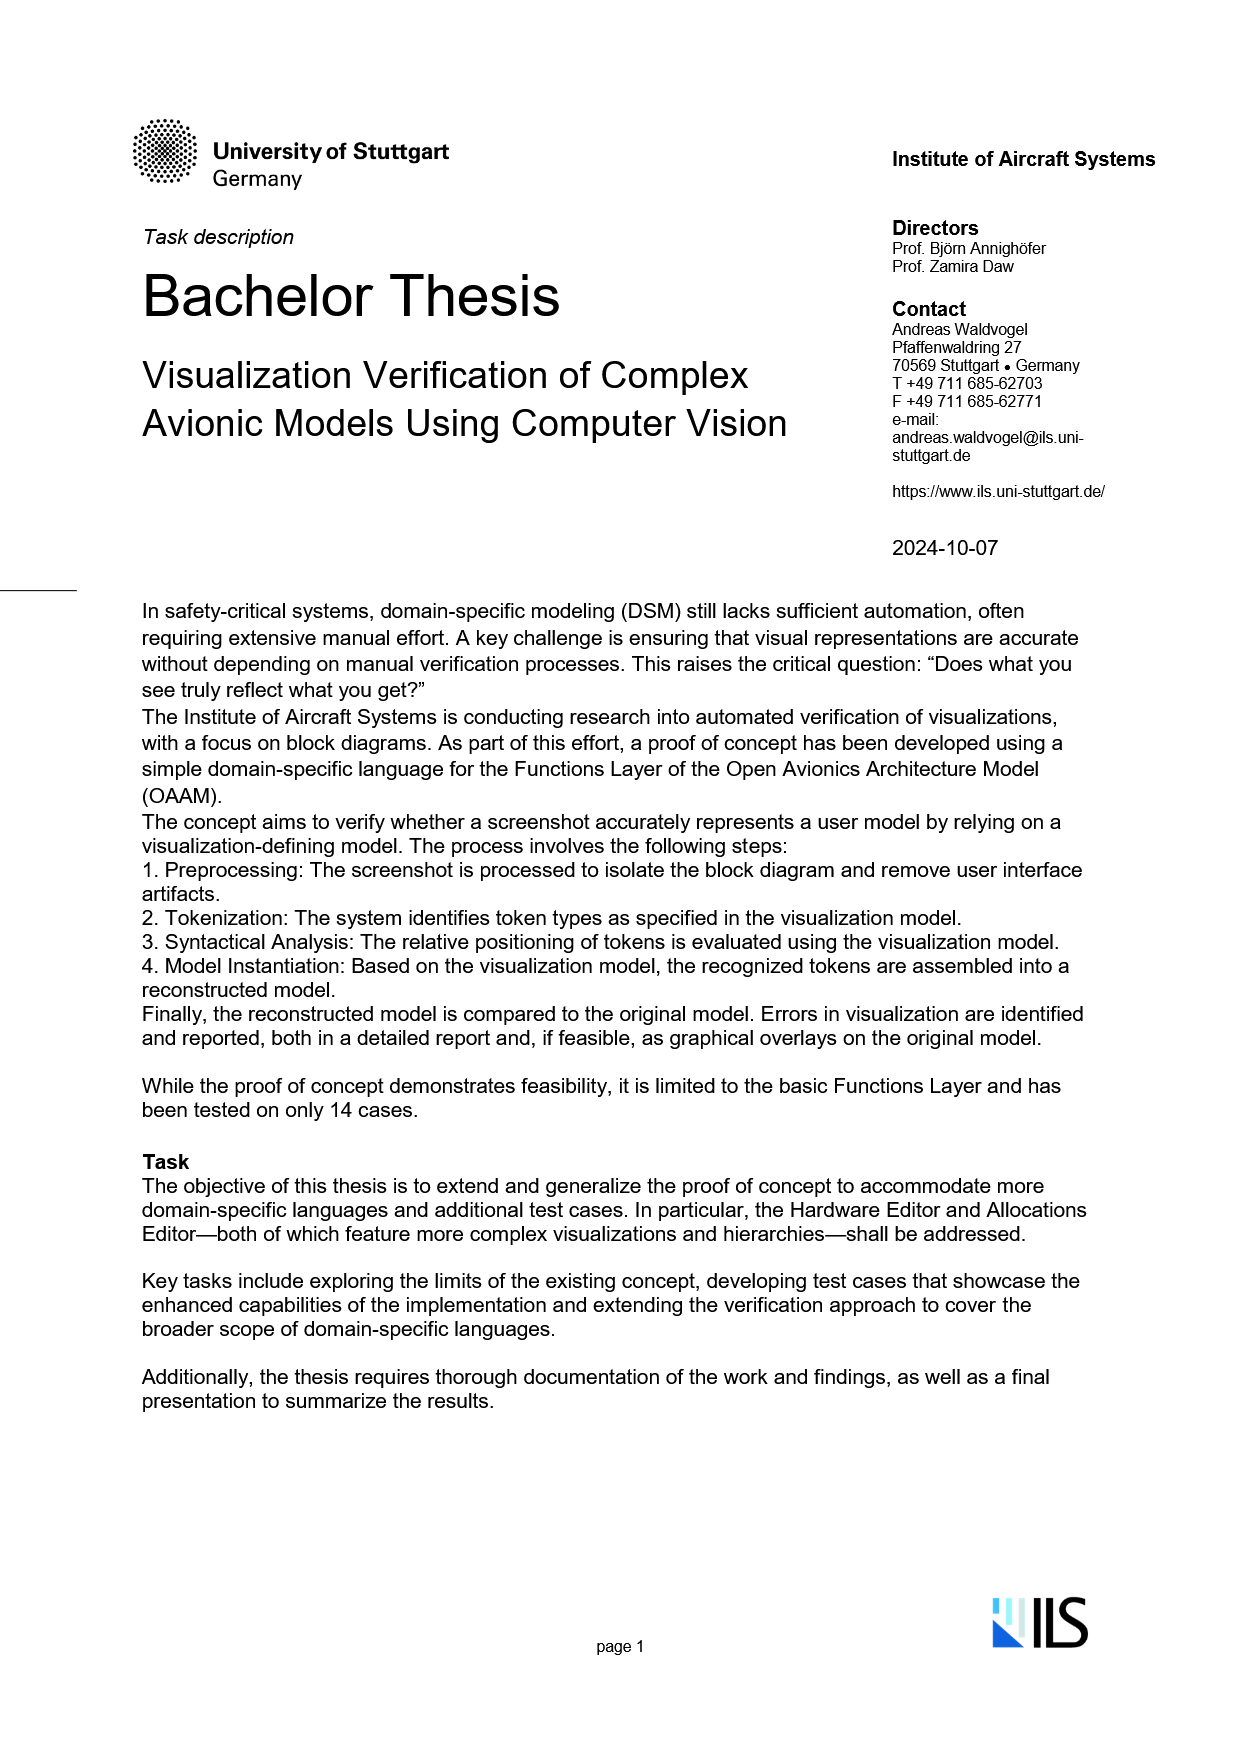
\includepdf[pages={1-2}]{Preamble/task.pdf}
\addchap*{Selbst{\"a}ndigkeitserkl{\"a}rung}

Hiermit versichere ich, dass ich diese Bachelorarbeit / Masterarbeit selbst{\"a}ndig mit Unterst{\"u}tzung des Betreuers/ der Betreuer angefertigt und keine anderen als die angegebenen Quellen und Hilfsmittel verwendet habe. Die Arbeit oder wesentliche Bestandteile davon sind weder an dieser noch an einer anderen Bildungseinrichtung bereits zur Erlangung eines Abschlusses eingereicht worden.

Ich erkl{\"a}re weiterhin, bei der Erstellung der Arbeit die einschl{\"a}gigen Bestimmungen zum Urheberschutz fremder Beitr{\"a}ge entsprechend den Regeln guter wissenschaftlicher Praxis\footnote{Nachzulesen in den DFG-Empfehlungen zur "`Sicherung guter wissenschaftlicher Praxis"' bzw. in der Satzung der Universit{\"a}t Stuttgart zur "`Sicherung der Integrit{\"a}t wissenschaftlicher Praxis und zum Umgang mit Fehlerverhalten in der Wissenschaft"'} eingehalten zu haben. Soweit meine Arbeit fremde Beitr{\"a}ge (z.B. Bilder, Zeichnungen , Testpassagen etc.) enth{\"a}lt, habe ich diese Beitr{\"a}ge als solche gekennzeichnet (Zitat, Quellenangaben) und eventuell erforderlich gewordenen Zustimmungen der Urheber zu Nutzung dieser Beitr{\"a}ge in meiner Arbeit eingeholt. Mit ist bekannt, dass ich im Falle einer schuldhaften Verletzung dieser Pflichten die daraus entstehenden Konsequenzen zu tragen habe.

\vspace{2cm}

Stuttgart, den \thedate \hfill \rule{8cm}{0.4pt} \linebreak
\mbox{~} \hfill	\theauthor

\addchap*{Nutzungsrechterkl{\"a}rung}

Hiermit erkl{\"a}re ich mich damit einverstanden, dass meine Bachelorarbeit / Masterarbeit zum Thema:
\begin{center}
	\textit{\thetitle}
\end{center}
in der Institutsbibliothek des Institutes f{\"u}r Luftfahrtsysteme mit sofortiger Wirkung {\"o}ffentlich zug{\"a}nglich aufbewahrt und die Arbeit auf der Institutswebseite sowie im Online-Katalog der Universit{\"a}tsbibliothek erfasst wird. Letzteres bedeutet eine dauerhafte, weltweite Sichtbarkeit der bibliographischen Daten der Arbeit (Titel, Autor, Erscheinungsjahr, etc.).

Nach Abschluss der Arbeit werde ich zu diesem Zweck meinem Betreuer neben dem Pr{\"u}fexemplar eine weitere gedruckte sowie eine digitale Fassung {\"u}bergeben.

Der Universit{\"a}t Stuttgart {\"u}bertrage ich das Eigentum an diesen zus{\"a}tzlichen Fassungen und r{\"a}ume dem Institut f{\"u}r Luftfahrtsysteme an dieser Arbeit und an den im Rahmen dieser Arbeit von mir erzeugten Arbeitsergebnissen ein kostenloses, zeitlich und {\"o}rtlich unbeschr{\"a}nktes, einfaches Nutzungsrecht f{\"u}r Zwecke der Forschung und der Lehre ein. Falls in Zusammenhang mit der Arbeit Nutzungsrechtsvereinbarungen des Instituts mit Dritten bestehen, gelten diese Vereinbarungen auch f{\"u}r die im Rahmen dieser Arbeit entstandenen Arbeitsergebnisse.

\vspace{2cm}

Stuttgart, den \thedate \hfill \rule{8cm}{0.4pt} \linebreak
\mbox{~} \hfill	\theauthor






\addchap*{Abstract}
\label{abstract}
{\LARGE Visualization Verification of Complex Avionic Models Using Computer Vision}

With the growing complexity of applications in aviation, the use of \acrlong{dsm} (\acrshort{dsm}) in the field has become vital. It enables engineers to work on larger and more complex applications more efficiently and, through automatic code generation, significantly reduces the number of errors in the resulting programs. For use in safety-critical applications however, \acrshort{dsm} requires significant verification effort. One important aspect of \acrshort{dsm} in these applications is ensuring a correct model visualization to increase safety and reduce the amount of manual verification work.\\
This thesis aims to improve the reliability of the automated verification of block-diagram visualizations in \acrshort{dsm}. Computer vision techniques are used to recognize and process block diagram models. The recognized data is compared with the original model to find and indicate deviations to the user inside a browser-based graphical model editor.\\
This thesis extends the capabilities of the block diagram recognition algorithm to work with complex and diverse diagrams in three graphical \acrlong{dsl}s (\acrshort{dsl}s). The new implementation is able to correctly identify and process intersecting or partially obscured lines in any orientation, detect a larger variety of vertices, and process text labels in multiple orientations, showcasing its potential to significantly reduce manual verification effort in \acrshort{dsm} applications.\\
The new implementation is evaluated using a set of 20 unique test cases, each containing one or two block diagrams with a single simulated error. The results show that the implementation is able to correctly identify and textually indicate all simulated errors to the user, differentiating between different error types. If possible, the implementation visually provides the position of the found errors inside the model editor alongside the textual indication.
\addchap*{Kurzzusammenfassung}
\label{kurzzusammenfassung}
{\LARGE Verifikation von Visualisierungen von komplexen Avionik Modellen mit Computer Vision}

Mit der steigenden Komplexit{\"a}t von Anwendungen in der Luftfahrt wird die Nutzung von \acrlong{dsm} (\acrshort{dsm}) in diesem Bereich immer wichtiger. Es erm{\"o}glicht Ingenieuren, effizienter an gr{\"o}{\ss}eren und komplexeren Anwendungen zu arbeiten und reduziert durch automatische Code-Generierung die Anzahl der Fehler in den resultierenden Programmen. Bei sicherheitskritischen Anwendungen jedoch ist \acrshort{dsm} durch die n{\"o}tige Verifikation der Modell-Visualisierungen mit signifikantem Mehraufwand verbunden.\\
Diese Arbeit zielt darauf ab, die Zuverl{\"a}ssigkeit der automatisierten Verifikation von Blockdiagramm-Visualisierungen in \acrshort{dsm} zu verbessern. Techniken der Computer-Vision werden verwendet, um Blockdiagramm-Modelle zu erkennen und zu verarbeiten. Die erkannten Daten werden mit dem urspr{\"u}nglichen Modell verglichen, um Abweichungen zu finden und dem Benutzer innerhalb eines browserbasierten grafischen Modelleditors anzuzeigen.\\
Diese Arbeit erweitert die bestehende Implementierung der Blockdiagramm-Erkennung, um mit komplexen und vielf{\"a}ltigen Diagrammen in drei grafischen \acrlong{dsl}s (\acrshort{dsl}s) zu arbeiten. Die neue Implementierung verwendet eine Kombination von Methoden aus der Computer-Vision, um Kreuzende oder teilweise verdeckte Verbindungslinien in verschiedenen Ausrichtungen, diverse Vertices in unterschiedlichen Gr{\"o}{\ss}en und Anordnungen sowie Textbl{\"o}cke in unterschiedlichen Orientierungen zu erkennen.\\
Diese Verbesserungen demonstrieren das Potenzial von Computer-Vision-Methoden, die Verifikation von \acrshort{dsm}-Modellen zu automatisieren und die Sicherheit in sicherheitskritischen Anwendungen der Luftfahrt zu erh{\"o}hen.\\
Die neue Implementierung wird anhand einer Reihe von 20 Testf{\"a}llen evaluiert, die jeweils ein oder zwei Blockdiagramme mit einem simulierten Fehler enthalten. Die Ergebnisse zeigen, dass die Implementierung in der Lage ist, alle simulierten Fehler korrekt zu identifizieren und textuell anzuzeigen, wobei zwischen verschiedenen Fehlertypen unterschieden wird. Wenn m{\"o}glich, gibt die Implementierung zus{\"a}tzlich zu der textuellen Anzeige auch die Position der gefundenen Fehler im Modelleditor visuell aus.

% Contents
\tableofcontents
% Figures
\listoffigures
% Tables
\listoftables
%Glossar
\printglossary[style=super,title=Glossary]
% Abbrevations
\glsaddall
\printglossary[type=\acronymtype,title=Index of abbreviations]
% Symbols and Units
\printglossary[type=symbolslist,style=symbunitlong,title={Index of Symbols and Units}]

\cleardoublepage
\pagenumbering{arabic}
\chapter{Introduction}
\label{chp:introduction}
Development of complex, safety-critical systems requires an efficient way for engineers to ensure the correctness and reliability of the developed software. \acrlong{dsm} (\acrshort{dsm}) provides an approach to achieve this by enabling the creation of models that are closely aligned with the specific concepts and requirements of a particular domain. This approach usually includes automatic code generation, which significantly reduces the risk of faulty applications \cite{waldvogel_2022}.\\
By using \acrshort{dsm}, engineers can work more effectively, as it allows for the abstraction of complex system details into more manageable and understandable representations. This not only enhances productivity but also the overall quality and safety of the developed systems.\\
Models can be represented visually using block-diagrams to further simplify the development process. Furthermore, \acrshort{dsm} enables the reuse of domain-specific knowledge and components.\\
In safety-critical domains, such as avionics, the ability to visualize models and automatically generate code from them ensures that the software adheres to safety standards and reduces the likelihood of human errors during the development process.

However, \acrshort{dsm} can only be used without subsequent manual verification, if the \acrshort{dsm} tools work correctly. This can either be achieved through time intensive qualified software development processes, which ensure an accurate and reliable visualization of \acrshort{dsm} through the tool itself, or through the use of unverified \acrshort{dsm} tools followed by the subsequent use of a small visualization verification tool to ensure the correctness of the application.\\
In low-cost projects with high safety requirements, a cost-effective qualification method is crucial, highlighting the potential of the latter approach for a qualifiable graphical verification tool for use in \acrshort{dsm} \cite{waldvogel_annighoefer_models_2024}.

A typical use case for \acrshort{dsm} in avionics could be a door opening system. The system consists of a door, a motor, a sensor and a control unit. The door can be opened and closed by the motor, which is controlled by the control unit. The sensor detects whether the door is open or closed. The control unit receives the sensor data and controls the motor accordingly.\\
This system can be modeled using a block diagram, where the door, motor, sensors and control unit are represented as blocks, and the connections between them are represented as lines. Another diagram can be used to model the airplanes hardware components and their connections, such as the core processing units, remote data concentrators, sensors and actuators. A third diagram can be used to allocate the functions to the hardware components, as well as the connections between them.\\
This diagram-based approach allows users to visualize the system and its components, making it easier to understand and communicate. Diagram-based model editors include well established tools such as \textit{Simulink} and \textit{Enterprise Architect}, which are widely used in the industry.

\chapter{Fundamentals}
\label{chp:fundamentals}
The following chapter provides an overview of the fundamentals of the technologies and concepts used in this thesis. It covers the \acrlong{xgee} (\acrshort{xgee}), computer vision, \acrlong{dsm} (\acrshort{dsm}), the challenges in \acrshort{xgee}'s visualization verification and the state of the art in automatic diagram interpretation.

\section{\acrlong{xgee} (\acrshort{xgee})}
\label{sec:xgee}
\textit{\acrshort{xgee}} is a graphical model editor, which is currently under development at the Institute of Aircraft Systems. This editor is designed to facilitate the creation and modification of ecore-based models through a browser-based graphical user interface. Generally, \acrshort{xgee} can be used to work with any kind of model, but this thesis focuses on its use in aviation.\\
The primary objective of \acrshort{xgee} is to provide a user-friendly platform that allows engineers to efficiently design and visualize complex avionic systems, possibly working simultaneously on the same model. A demonstrator of \acrshort{xgee} is currently available online.\footnote{\url{https://xgee.de/en/}}\\
Within \acrshort{xgee}, three distinct types of \textit{tokens} are utilized across three specialized editors to represent various components of avionic models. These editors are:
\begin{itemize}
    \item signals
    \item vertices
    \item text labels
\end{itemize}
We consider \acrshort{xgee} editors for three layers of the \acrlong{oaam} (\acrshort{oaam}): the functions editor, the hardware editor and the allocations editor. \acrshort{oaam} supports additional layers such as the \textit{restrictions layer} and \textit{capabilities layer}, which are not considered in this thesis.\\
In \textit{\acrshort{xgee}}, each of the three editor models utilizes a unique set of \textit{.svg} files to represent different components within the avionic model. These editor models are the \textit{functions editor}, the \textit{hardware editor}, and the \textit{allocations editor}. An overview of these editors is provided in the following sections.

\subsection{Functions editor}
\label{sec:functions_editor}
\begin{figure}[h]
    \centering
    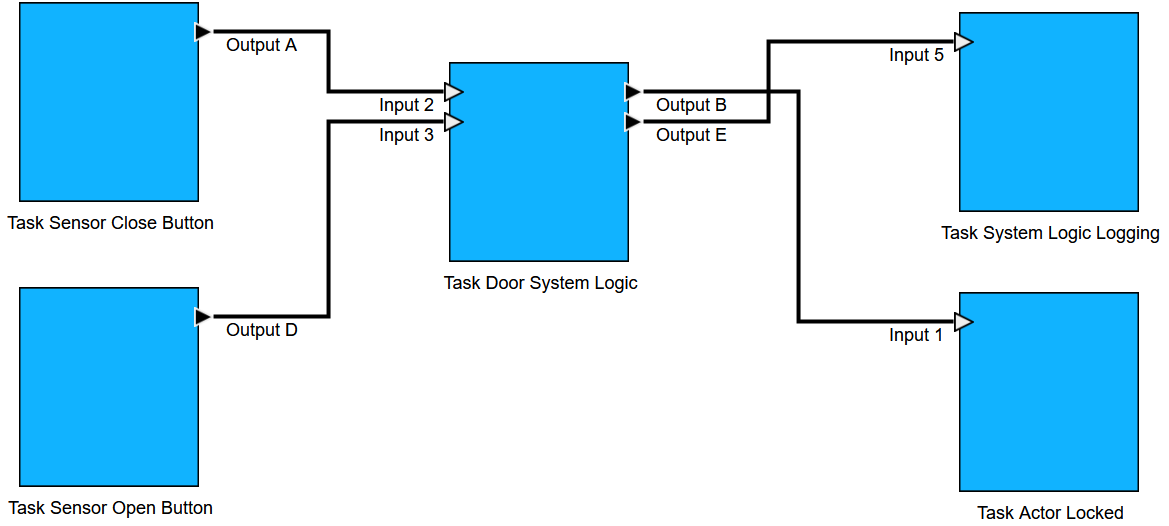
\includegraphics[width=0.4\textwidth]{pictures/functions_editor.png}
    \caption[Example of a diagram in the Functions editor]{Example of a diagram in the Functions editor.}
    \label{fig:functions_editor}
\end{figure}
The functions editor is used to define avionic functions and their interactions. Functions are represented as large blue boxes, with their interactions shown through black signals connecting inputs and outputs. Inputs and outputs are depicted as small black-and-white triangles located on the left and right edges of the function boxes. Inputs, outputs and functions have visible text labels (see \autoref{fig:functions_editor}).

\subsection{Hardware editor}
\label{sec:hardware_editor}
\begin{figure}[h]
    \centering
    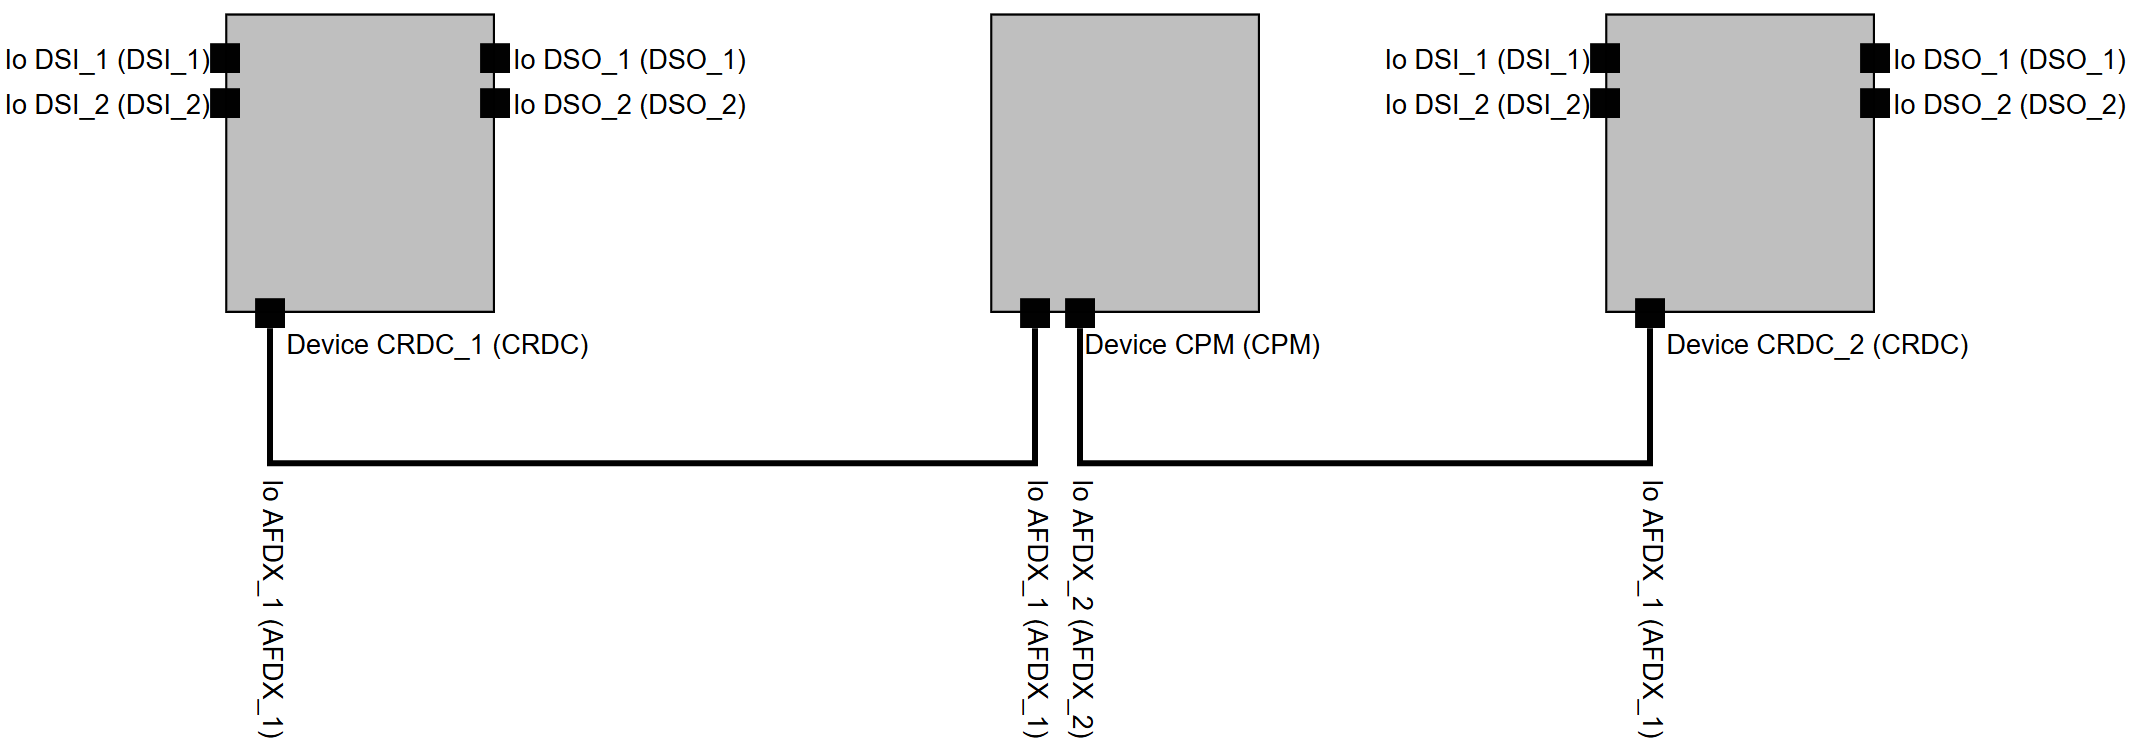
\includegraphics[width=0.4\textwidth]{pictures/hardware_editor.png}
    \caption[Example of a diagram in the Hardware editor]{Example of a diagram in the Hardware editor.}
    \label{fig:hardware_editor}
\end{figure}
The hardware editor is used to define hardware components and their physical connections. Hardware components are represented as large gray boxes, and their connections are illustrated as black signals linking \acrlong{io} (\acrshort{io}) ports. These \acrshort{io} ports appear as small black squares positioned along any edge of the hardware boxes. Like in the functions editor, \acrshort{io}s and devices have visible text labels (see \autoref{fig:hardware_editor}).

\subsection{Allocations editor}
\label{sec:allocations_editor}
\begin{figure}[h]
    \centering
    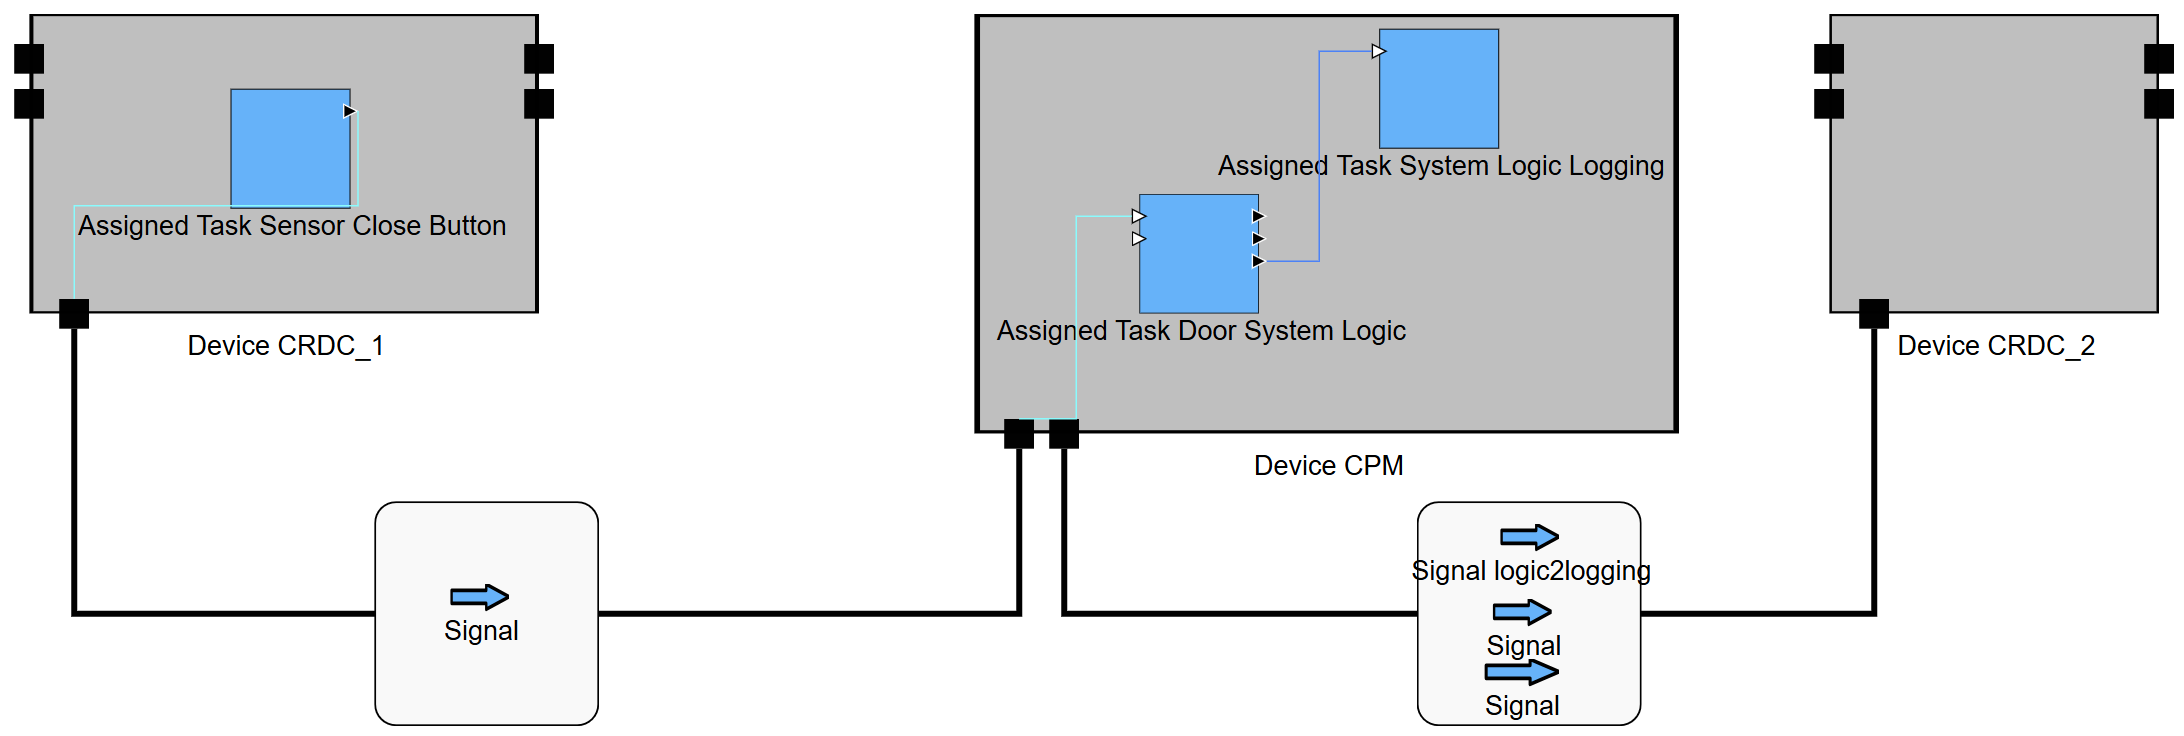
\includegraphics[width=0.4\textwidth]{pictures/allocations_editor.png}
    \caption[Example of a diagram in the Allocations editor]{Example of a diagram in the Allocations editor.}
    \label{fig:allocations_editor}
\end{figure}
The allocations editor is used to map functions to hardware components. Visually, it is simmilar to the hardware editor, with allocated functions represented as small blue boxes nested within larger gray hardware boxes. The specific signal transmissions between the hardware components are illustrated as white signal containers that overlap with the corresponding physical connections. These boxes contain the signals being transmitted through the corresponding connection. Inside the gray hardware boxes, connections between functions and \acrshort{io}'s, are illustrated as thin, color-coded signals. They represent the same connections proviously defined in the functions editor, but are now allocated to specific hardware components (see \autoref{fig:allocations_editor}).

This thesis builds upon the work of Andreas Waldvogel and Bj{\"o}rn Annigh{\"o}fer in \cite{waldvogel_annighoefer_models_2024} to further automate the verification process within \acrshort{xgee} by tokenizing a screenshot of the editor window. This means detecting the bounding boxes and token types of all elements of the diagram. To recognize and process the screenshot data, methods from the Python library \textit{\acrshort{opencv}} are being used.\\
The complete process of converting a screenshot of a block-diagram into meaningful error indications requires a series of individual steps, as shown in \autoref{fig:visualization_steps}.\\
By rebuilding a model from the recognized tokens and comparing it to the original, visualization errors become apparent and can be indicated to the user, including issues such as unclear signal intersections, signals being obscured by blocks, text labels being obscured by signals or blocks, blocks being scaled down to the point of disappearing, or blocks obscuring other blocks.\\
Fundamentally, this verification approach can be applied to any model-based application like Simulink. However, implementing the model comparison step would require much work, as the model has to be reconstructed from the recognized tokens, which is not trivial.\\
The goal of this thesis is to provide a tool that can be used to verify the correctness of the visualization of avionic models within \acrshort{xgee}'s functions and hardware editors, enabling engineers to work more effectively and with a higher degree of confidence.
\begin{figure}[h]
    \centering
    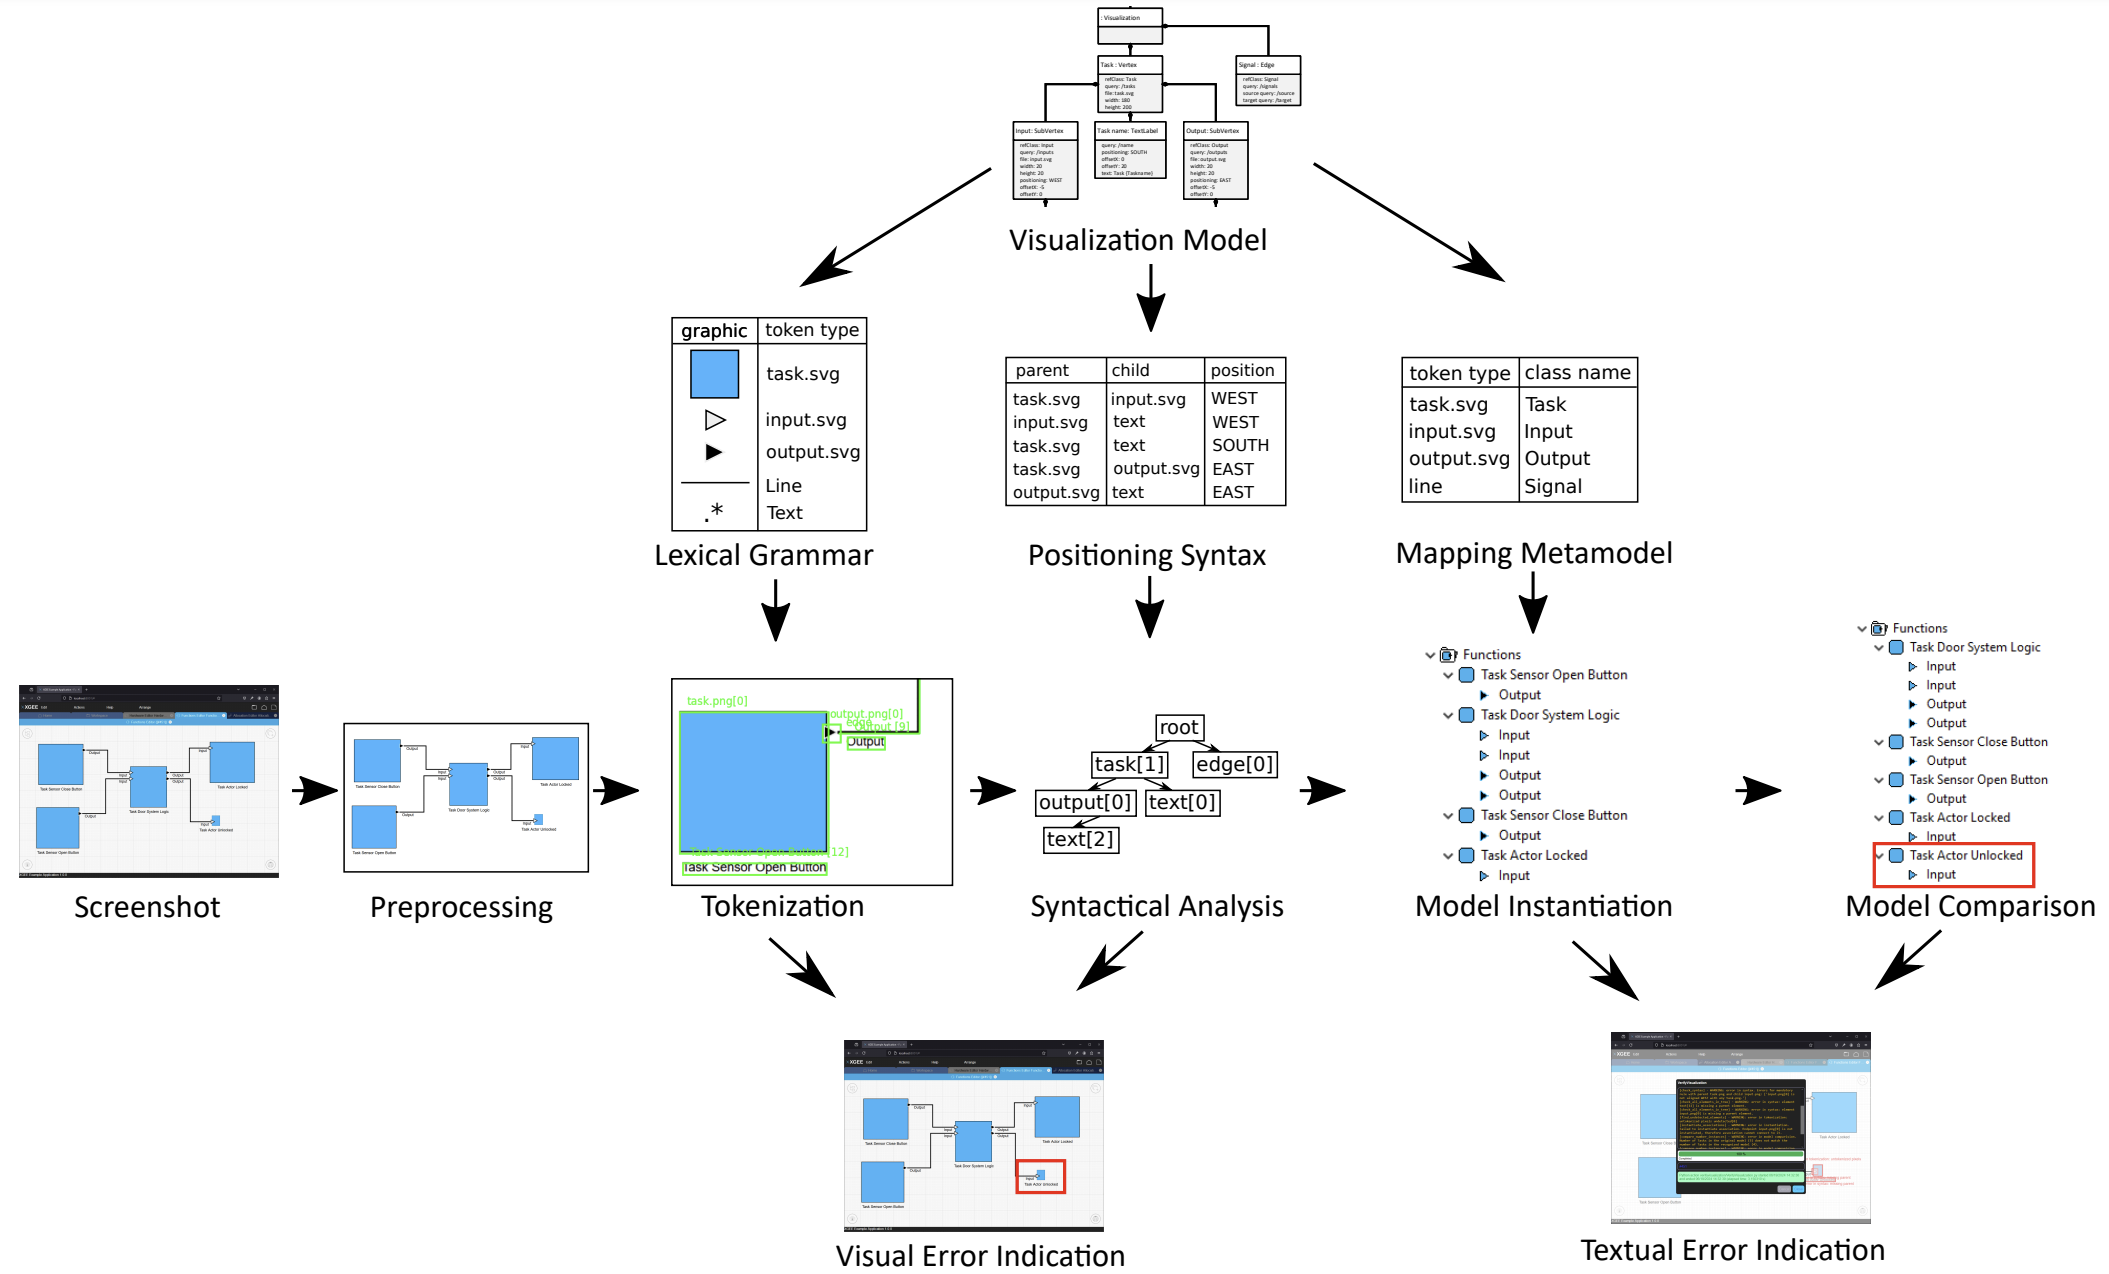
\includegraphics[width=0.9\textwidth]{pictures/visualization_steps.png}
    \caption[Steps in the visualization verification process]{Steps in the visualization verification process \cite{waldvogel_annighoefer_models_2024}.}
    \label{fig:visualization_steps}
\end{figure}

\section{Computer Vision}
\label{sec:computer_vision}
Humans have the remarkable ability to efficiently perceive and interpret visual information, extracting meaningful insights from their surroundings with ease. Tasks such as recognizing familiar faces, estimating distances, or identifying irregularities in a road surface may appear trivial to us, yet they present a significant challenge for computers to replicate.\\
Computer Vision is the field of mathematical models and approaches that enable computers to recover, interpret, and understand information from images or videos like humans. It encompasses a wide range of tasks, including image recognition, object detection, automation and more. It has numerous applications in a variety of fields, such as autonomous vehicles, facial recognition and medical imaging. Eventhough the field has made significant progress in recent years, many challenges such as handeling complex environments in real-time, detecting objects in low-light conditions or interpreting ambiguous data remain unsolved.\\
In avionic model development, visual representations of models are used to communicate complex systems and their interactions. To ensure correctness of these models, computer vision tools are used to interpret and verify the visual model representations, eliminating the need for manual verification.

\section{\acrlong{dsm}}
\label{sec:domain_specific_modeling}
When developing safety-critical real-world applications, such as an avionics system, \acrlong{oop} (\acrshort{oop}) enables developers to create complex systems by defining classes and objects that interact with each other. However, as the complexity of these systems increases, it becomes harder for many developers to collaborate on the same project, as they need to understand the entire system to make changes.\\
\begin{figure}[h]
    \centering
    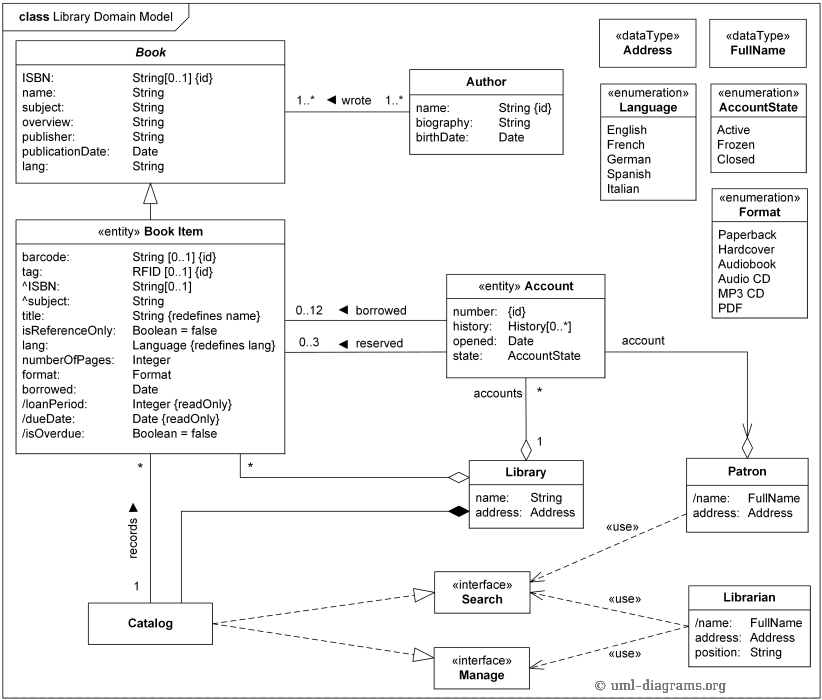
\includegraphics[width=0.6\textwidth]{pictures/uml_class_diagram.png}
    \caption[Example of an \acrshort{uml} class diagram]{Example of an \acrshort{uml} class diagram describing a library management system. In highly specialized domains, such as avionics, an \acrshort{uml} diagram might be too abstract to clearly represent the system. \cite{uml_diagrams_2016}}
    \label{fig:uml_diagram}
\end{figure}
The \acrlong{uml} (\acrshort{uml}) is a generic and source-code-independent \acrshort{oop} description language that can be used to model software systems. It provides a standardized way to visualize the design of a system using \acrshort{uml} diagrams, making it easier to understand and communicate. These diagrams consist of clearly defined elements specified in the \acrshort{uml} standard and can be directly converted to code through automatic code generation.\\
\autoref{fig:uml_diagram} shows an example \acrshort{uml} class diagram describing a library management system.\\
While \acrshort{uml} provides a standardized approach for modeling software systems in a general-purpose manner, it may not fully address the specific needs of highly specialized domains, such as avionics. Domain-Specific Modeling (\acrshort{dsm}) addresses this issue by enabling engineers to create models that are closely aligned with the concepts and requirements of a particular domain. For example, in avionics systems, \acrshort{dsm} might use specialized notation to represent specific aircraft components, such as sensors, actuators, or flight control systems, rather than relying on abstract classes and objects like \acrshort{uml}. This reduces the semantic gap between the model and the real-world implementation.\\
In most cases, a \acrlong{dsl} (\acrshort{dsl}) is developed by a small group of experts within a company or within a collaboration between companies and tailored to their unique needs, then used consistently throughout the organization to ensure uniformity and efficiency. This approach simplifies design processes and ensures that models are more easily validated, improving both reliability and safety, both critical requirements in the development of avionics systems.

\section{Challenges in \acrshort{xgee}'s visualization verification}
\label{sec:challenges_xgee_visualization_verification}
The \acrshort{xgee} editor is a browser-based model editor that, in our application, allows users to create and edit avionic models using a graphical interface but in general, \acrshort{xgee} can be used to edit anything that uses an ecore metamodel. For this thesis, we conside three editor models: the functions editor, the hardware editor and the allocations editor, each useing a different set of tokens to represent different elements of the model.\\
To verify the correctness of this visualization, a screenshot of the model is tokenized, meaning that the bounding boxes and token types of all elements of the diagram are detected. The recognized tokens are checked for correct syntax and unrecognized pixels. Then they are used to rebuild the model and compare it to the original, highlighting any visualization errors.\\
The primary challenge addressed in this paper is the accurate detection of these tokens. This includes handling intersecting and overlapping signals, obscured vertices and text labels, as well as large and complex models.\\
Furthermore, the integration of new methods for token detection into the existing codebase introduces an additional layer of complexity. 
Another challenge adressed in this thesis is to make the verification more versatile by enabeling it to change with the model. This is achieved by making the verification \textit{model-driven}, allowing the methods to query the current model for information and dynamically change their behavior based on it.

\section{State of the Art}
\label{sec:state_of_the_art}
Automatic diagram interpretation has been a topic of interest in the field of computer vision and \acrshort{dsm}. It could enable engineers to utilize diagrams that are currently only available as images or drawings, which would otherwise require manual reverse engineering. However, in large projects with consistent and well-maintained databases, most diagrams are already stored in usable formats, reducing the practical demand for automatic diagram interpretation in the industry. Consequently, no commercial tools for verified block diagram recognition are currently available on the market.

The work most similar to this thesis is presented in \cite{mani_haddad_constantini_douhard_li_poirier_2020}, which utilized a specifically trained \acrlong{cnn} to classify common symbols used in \textit{Piping and Instrumentation Diagrams}, achieving an accuracy of 90$\%$. They detected connecting lines using a graph search approach. By representing the pixels within the diagram image as a graph of black and white nodes, connecting lines can be identified by starting at any node corresponding to a symbol and traversing the diagram graph along its black nodes, keeping track of connected symbols along its path. For text detection, they used \textit{\acrshort{east}}, a text detectrion pipeline using a neural network. However, their method did not address the indication of uncertainties to the user. Instead, their primary goal was to digitize a database of diagrams to enable applications such as diagram search and machine learning-based predictive maintenance in the industry.\\
Recent research has focused on the recognition of handwritten diagrams, mathematical equations, flowcharts, and circuit diagrams. For example, \cite{wei_phung_bouzerdoum_bermak_2015} proposed a method for normalizing images captured by hand at arbitraty orientations to improve recognition accuracy and reliablity.\\
\cite{schaefer_keuper_stuckenschmidt_2021} used \textit{Arrow \acrshort{rcnn}}, a deep-learning model and an extension of the \textit{\acrlong{rcnn} (\acrshort{rcnn}) object detector} \cite{zhang2023dive} to detect and classify offline handwritten diagrams. \textit{\acrshort{rcnn}} is an object detection framework to identify bounding boxes around objects and classify each object into its respective category. On a scanned flowchart dataset, the model achieved an accuracy of 78.6$\%$, substantially improving the previous state of the art. However, their method was not designed recognize the diagrams structure or to adress the specific challenges of avionic model diagrams, particularly the need for validation and user feedback mechanisms.\\
Building on this work, \cite{fang_feng_cai_2022} proposed \textit{DrawnNet}, a \acrshort{cnn} and keypoint-based detector capable  of recognizing both symbols and diagram structures. Among other techniques, \textit{DrawnNet} leverages arrow direction predictions to enhance diagram interpretation.\\
\cite{yang_wang_zhang_li_wang_yang_shi_2024} proposed a framework for \acrlong{sld} (\acrshort{sld}) recognition, which are used in electrical engineering to represent power systems. Their methods include decomposing the diagram into seperate layers of electrical symbols and text labels to mitigate interference, using \acrshort{rcnn} to identify graphical symbols and the \textit{super-resolution} technique to improve text label recognition.

The approaches discussed above face challenges due to the inherent ambiguity of loosely defined graphical modeling languages and non-ideal photos of diagrams. A significant amount of effort is typically spent on recognizing various styles, but they often prioritize maximizing detection without considering the level of confidence in the results. In contrast, our approach takes a different direction. By leveraging the precise definition of a graphical \acrlong{dsl} (\acrshort{dsl}), we focus on a more structured verification process. Rather than attempting to recognize all elements, our goal is to highlight areas where uncertainty exists in the visualization, providing more meaningful and targeted feedback.
The methods proposed in this thesis are based on the work of \cite{waldvogel_annighoefer_models_2024}, which introduced a method for tokenizing and validating a screenshot of an avionic model within the \acrshort{xgee} editor. The aim of this thesis is to extend this work by improving the accuracy of token detection and integrating new methods for more complex detection tasks.  
\chapter{Advanced Block Diagram Recognition}
\label{chap:new_concepts}
Accurately interpreting complex diagrams is essential for many analytical and computational tasks. In the context of \acrshort{xgee}, this involves breaking down screenshots into meaningful components through tokenization. This process, however, depends on the robustness and reliability of the underlying algorithms. This chapter aims to build upon the original algorithms, improving upon their detection accuracy, versatility and ensuring stability.

\section{Edge Detection}
\label{sec:edge_detection}
Edges represent connections between vertices, inputs and outputs. Detecting edges accurately requires an approach that can identify individual line segments and how they connect to form complex chains. This section introduces a robust edge detection pipeline leveraging multiple computer vision techniques to reliably identify edges across a wide variety of block diagrams within \acrshort{xgee}.
\begin{wrapfigure}{R}{0.4\textwidth}
    \centering
    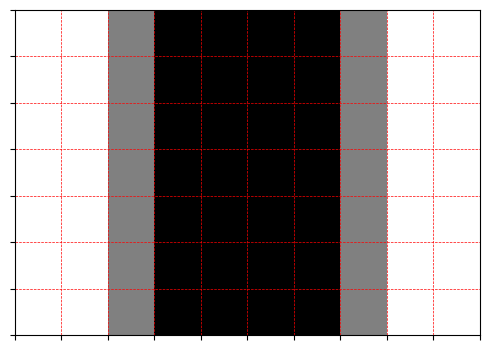
\includegraphics[width=\linewidth]{pictures/kernel_ver.png}
    \caption[Kernel used for vertical edge detection]{kernel used for vertical edge detection, rotated by 90\textdegree\ to generate the horizontal kernel.}
    \label{fig:kernel_ver}
\end{wrapfigure}

\subsection{Kernel-based Edge Detection}
\label{sec:kernel_edge_detection}
Since there are only vertical and horizontal edges within \acrshort{xgee}, two different kernels are used to find all pixels containing part of a vertical or horizontal edge. The \textit{filter2D()} function places the kernel anchor (usually the top left value of the kernel) on top of a pixel, with the rest of the kernel overlapping the corresponding local pixels. The kernel values are then multiplied by the corresponding pixel values underneath and added together. The result is saved and placed on the location of the anchor. The vertical kernel in \autoref{fig:kernel_ver} is rotated by 90$^{\circ}$ to generate the horizontal kernel.\\
The same process can be expressed using \autoref{eq:filter2D}, where $H$ is the resulting matrix, $I$ is the original image and $K$ is the used kernel, with $x$, $y$, $i$ and $j$ representing individual pixels within the image and the kernel. This process is repeated for every pixel and, depending on the structure of the kernel, it can also be used to blur or sharpen an image \cite{opencv_filter2d_2024}.\\
Currently, only a single line width defined by the kernel size is supported, which is enough for the functions and hardware editor. The allocations editor, however, will require support for multiple line widths and low contrast lines.\\
Each value in the processed image is normalized to an 8-bit integer between 0 and 255. This allows the data to be visualized as a gray scale image and processed further using \acrshort{opencv}'s \textit{thresholding()} function to extract the detected pixels (see \autoref{fig:filter2d} and \ref{fig:threshold}).\\
As illustrated in \autoref{fig:comparison_filter}, ports and letters are sometimes misidentified as edges. Additionally, intersections of edges as well as points where horizontal and vertical edges meet are not immediately detected. These challenging areas will be processed individually in a later step in the edge detection pipeline. Apart from these specific cases, the method effectively extracts all pixels corresponding to vertical and horizontal edges, provided their widths match those of the used kernels.
\begin{equation}
\label{eq:filter2D}
    H(x, y) = \sum_{i=0}^{M_i-1} \sum_{j=0}^{M_j-1} I(x + i - a_i,y + j - a_j) \cdot K(i, j)
\end{equation}

\begin{figure}[htb]
    \centering
    \includegraphics[width=1\linewidth]{pictures/filter2D.png}
    \caption[Filter2D function results for the horizontal and vertical kernel]{Filter2D function results for the horizontal (left) and vertical (right) kernel before thresholding. \textit{Edge-like} pixels are colored more yellow, while \textit{non-edge-like} pixels are colored more purple.}
    \label{fig:filter2d}

    \centering
    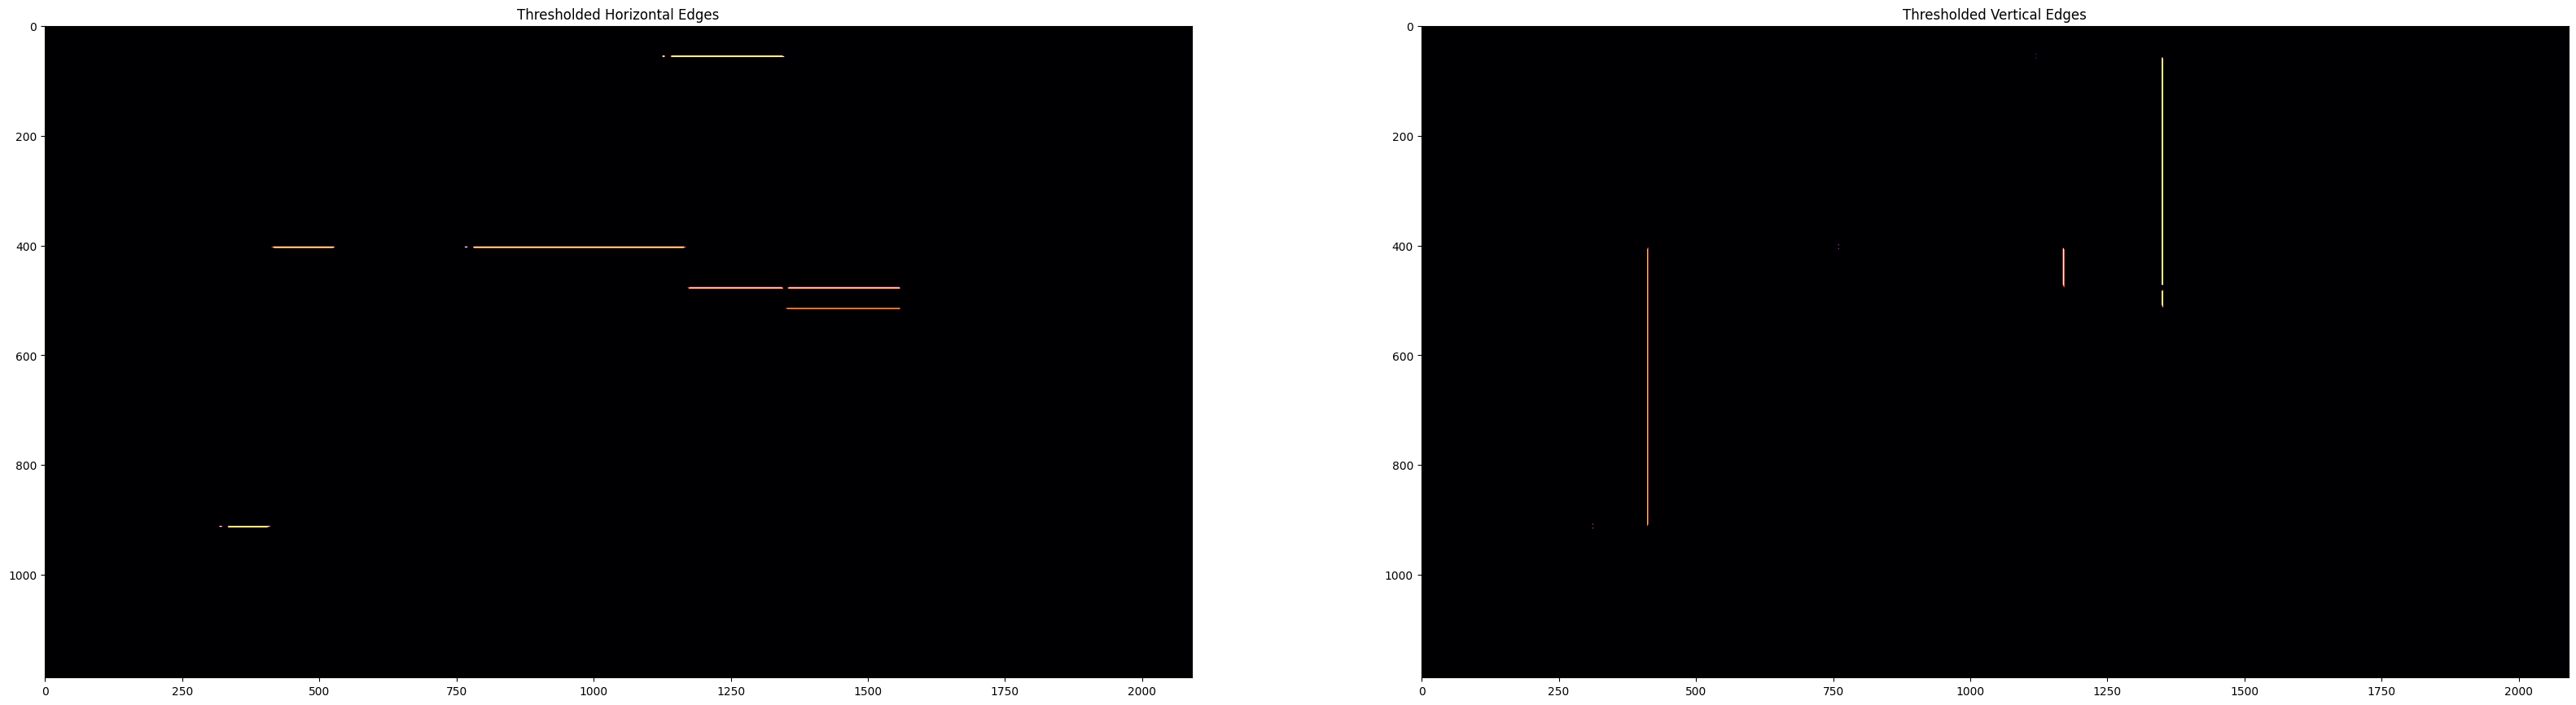
\includegraphics[width=1\linewidth]{pictures/threshold.png}
    \caption[Filter2D function results for the horizontal and vertical kernel thresholded]{Thresholded filter2D function results. \textit{Edge-like} pixels are now isolated.}
    \label{fig:threshold}
\end{figure}
For easier subsequent processing and data storage, the thresholded pixels seen in \autoref{fig:threshold} are converted to line segments consisting of start- and endpoints. This is achieved through two of \acrshort{opencv}'s built-in functions:\\
\textit{findContours()}, which retrieves contours from a binary image using an algorithm introduced by Satoshi Suzuki and others in \cite{suzuki_1985}. In this context, it is used to group nearby pixels and represent them as narrow polygons.\\
\textit{approxPolyDP()}, which approximates a curve or a polygon with another curve or polygon with less vertices using an algorithm introduced by David H Douglas and Thomas K Peucker in their paper: \cite{douglas_peucker_1973}. This function is used to simplify the contours found by \textit{findContours()} into line segments.
\begin{figure}[ht]
  \centering
  \begin{minipage}[b]{0.45\textwidth}
    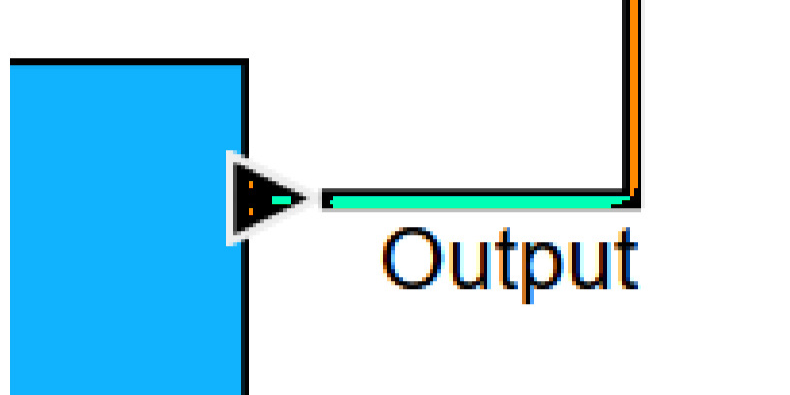
\includegraphics[width=\textwidth]{pictures/thresh_zoom.png}
  \end{minipage}
  \hfill
  \begin{minipage}[b]{0.45\textwidth}
    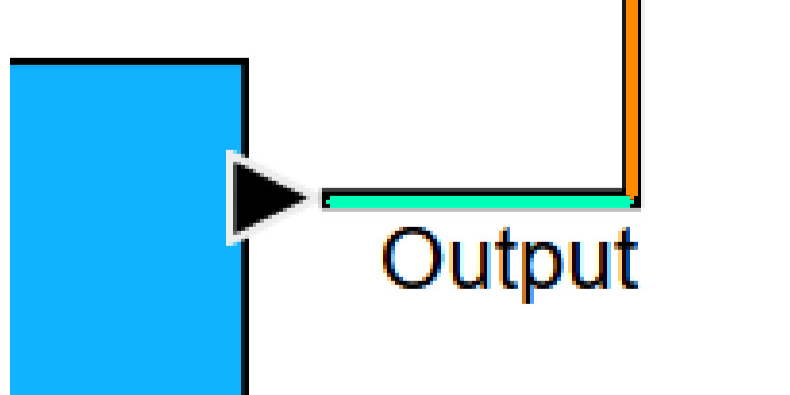
\includegraphics[width=\textwidth]{pictures/line_segments_zoom.png}
  \end{minipage}
  \caption[Detected pixels / line segments before and after filtering]{Comparison of detected pixels and line segments around an output before and after filtering short segments.}
  \label{fig:comparison_filter}
\end{figure}
\begin{figure}[ht]
    \centering
    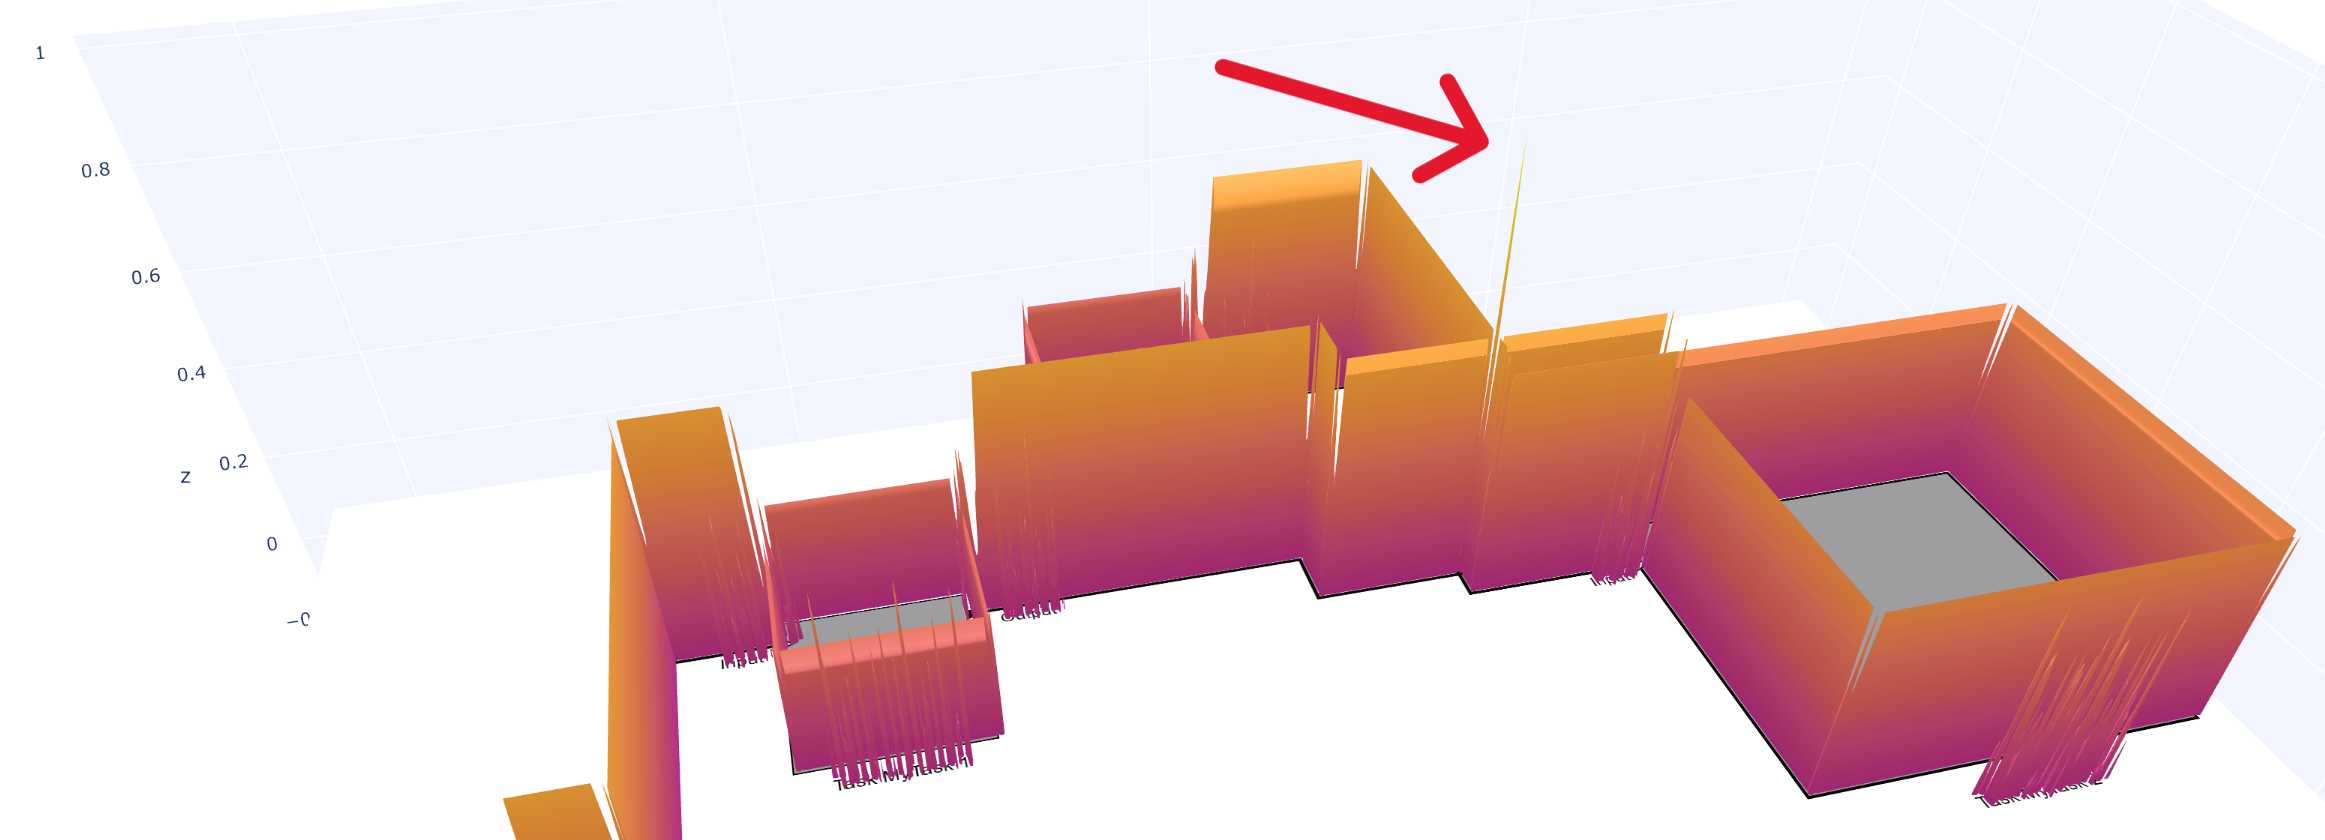
\includegraphics[width=1\linewidth]{pictures/intersection_peak.png}
    \caption[Similarity score peak at an intersection]{Similarity score peak at an intersection visualized in 3d using \textit{plotly}. X and Y axes show the screenshot in grayscale, while the Z axis represents the similarity score.}
    \label{fig:intersection_peak}
\end{figure}\\
Misidentified letters and ports are removed by filtering out all line segments with a length shorter than 20 pixels. In all test cases, this approach successfully removes the unwanted line segments while keeping the edges, illustrated in \autoref{fig:comparison_filter}.

\newpage
\subsection{Intersection Detection}
\label{sec:intersection_detection}
\begin{wrapfigure}{R}{0.4\textwidth}
    \centering
    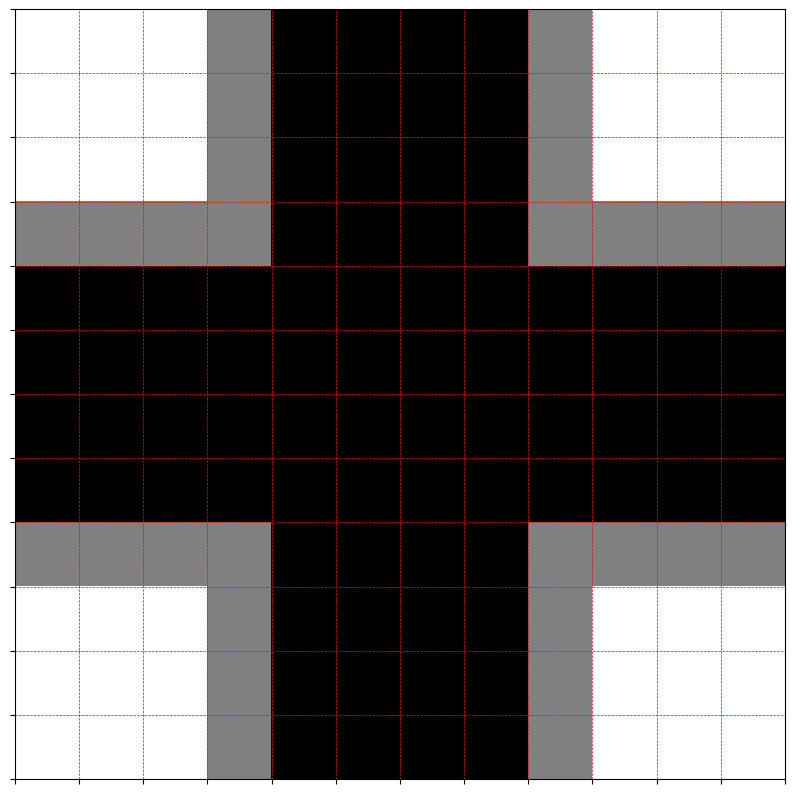
\includegraphics[width=\linewidth]{pictures/intersection_template.png}
    \caption[Intersection detection template]{Template image used for intersection detection.}
    \label{fig:intersection_template}
\end{wrapfigure}
As shown in \autoref{fig:threshold}, the \textit{filter2D()} function initially does not detect any edges at intersections, leading to gaps between the line segments. To process these gaps, it is assumed that intersections always consist of two straight edges. Overlapping 90\textdegree\ turns are considered impossible and will result in an error caused by the incorrect edge recognition, as it would result in an ambiguous diagram.\\
First, all intersections in the image are detected using \acrshort{opencv}'s \textit{matchTemplate()} function, which matches a template image of an intersection, as seen in \autoref{fig:intersection_template}, to overlapping regions of the target image \cite{opencv_matchTemplate_2024}.\\
The function slides the template across the image, comparing overlapping patches with the template using a specified method. Among the available methods \cite{opencv_comparison_methods_2024}, \textit{Sum of square differences normed} (\textit{tm\_sqdiff\_normed}) produced the most accurate results. For each pixel, according to \autoref{eq:sqdiff_normed}, the function calculates and assigns a value $R(x, y)$ representing the similarity between the template $T(x', y')$ and the corresponding image region $I(x + x', y + y')$ below. While this approach is more precise than \textit{filter2D()}, it is also significantly more resource-intensive.
\begin{equation}
    \label{eq:sqdiff_normed}
    R(x,y) = \frac{\sum_{x',y'} (T(x',y') - I(x + x', y + y'))^2}{\sqrt{\sum_{x',y'} T(x',y')^2 \cdot \sum_{x',y'} I(x + x', y + y')^2}}
\end{equation}
% \begin{wrapfigure}{R}{0.4\textwidth}
%     \centering
%     
\includegraphics[width=\linewidth]{pictures/aliasing.png}
%     \caption[Aliasing example found near hard edges]{Aliasing typically found near hard edges to increase the apparent resolution or contrast. The shade of gray is not the same on both sides of the edge.}
%     \label{fig:aliasing}
% \end{wrapfigure}
At intersections, the similarity value is approximately 85$\%$. This slight discrepancy likely arises from how modern operating systems use aliasing to render text and lines with higher apparent resolution and contrast compared to the display. Zooming in (see \autoref{fig:aliasing}) reveals that the white pixels near edges and text are often replaced with subtle color hues or shades of gray.\\
Rendering the results of the template matching highlights a peak in similarity at the intersection (\autoref{fig:intersection_peak}). Thresholding isolates this peak, typically yielding two or more matches per intersection. These matches are then filtered based on proximity, ensuring only one match is detected at each intersection.\\
The method then processes each detected intersection by connecting the two vertical and two horizontal line segments adjacent to it. This eliminates any residual points near the intersection, leaving only one vertical and one horizontal line segment, as illustrated in \autoref{fig:intersection_before_after}.

\subsection{Container Detection}
\label{sec:container_detection}
\begin{figure}[ht]
    \centering
    \begin{minipage}[t]{0.45\textwidth}
        \vtop{\hbox{
\includegraphics[height=0.2\textheight]{pictures/aliasing.png}}}
        \caption[Aliasing example found near hard edges]{Aliasing typically found near hard edges to increase the apparent resolution or contrast. The shade of gray is not the same on both sides of the edge.}
        \label{fig:aliasing}
    \end{minipage}
    \hfill
    \begin{minipage}[t]{0.45\textwidth}
        \vtop{\hbox{
\includegraphics[height=0.2\textheight]{pictures/container_template_mask.png}}}
        \caption[Signal container detection template]{Template image used for signal container detection. The red area illustrates pixels ignored during template matching.}
        \label{fig:container_template}
    \end{minipage}
\end{figure}
In the allocations editor, the same approach is applied to detect and process signal containers on top of edges. To enhance diagram readability, it is assumed that no 90\textdegree\ turns are concealed behind the containers, only one edge passes behind each container and that edges pass through them in a straight line, avoiding ambiguities that could confuse both computer vision algorithms and human users. The primary distinction from intersection detection lies in the number of line segments: at a signal container, only two line segments meet, rather than four.\\
The method detects all signal containers in the screenshot using template matching. To ignore any pixels in the center of the container template, a mask (illustrated in red in \autoref{fig:container_template}) is used. This allows \textit{signal arrow vertices}, indicating signals traveling through the underlying connection, to overlap with the container vertices, without causing any interference with the detection process. The detected containers are then processed in the same way as intersections, connecting the two line segments adjacent to the container.
\begin{figure}[ht]
    \centering
    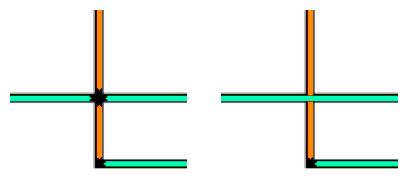
\includegraphics[width=0.7\linewidth]{pictures/intersection_before_after.png}
    \caption[Intersection before and after connecting line segments]{Intersection before and after connecting the line segments.}
    \label{fig:intersection_before_after}
\end{figure}
\newpage
\subsection{Line Segment Grouping and Sorting}
Converting the line segments into polylines at this stage would produce unusable data, as the segments are not grouped and not sorted in the sequential order of the edge's \textit{flow}. To generate proper polylines, the line segments must first be grouped into multiple lists of connected chains which then have to be sorted into the correct order. For instance, if the first line segment in the list is an intermediate segment within an edge, the polyline function may mistakenly attempt to connect its endpoints directly to the next point in the list, without considering whether it belongs to the same continuous chain, resulting in incorrect edge detections.\\
The implemented method begins by selecting the first line segment, adding it as a starting point to the first chain group and to a list of used segments and setting the \textit{chain\_growing} flag to true. It then iterates through all remaining segments, checking whether each segment has already been used and whether any of its points lie within 7 pixels of the points of the current segment. If a match is found, the segment is added to the \textit{used\_segments} list and the current chain group. If no segment is found within the 7-pixel threshold, the \textit{chain\_growing} flag is set to false, and the completed chain group is added to the list of chains (see \autoref{lst:grouping_line_segments}). A threshold of 7 pixels was selected as it reliably produces connected polylines while ensuring that closely positioned lines, such as those at ports, remain distinct and separate. This process continues until all line segments have been assigned to a group, illustrated with colors in \autoref{fig:chains_before_after}.
\lstinputlisting[language=Python, firstline=9, lastline=34, caption={Grouping line segments into line segment chains.}, label = {lst:grouping_line_segments}]{layout/code.m}
\begin{figure}[ht]
    \centering
    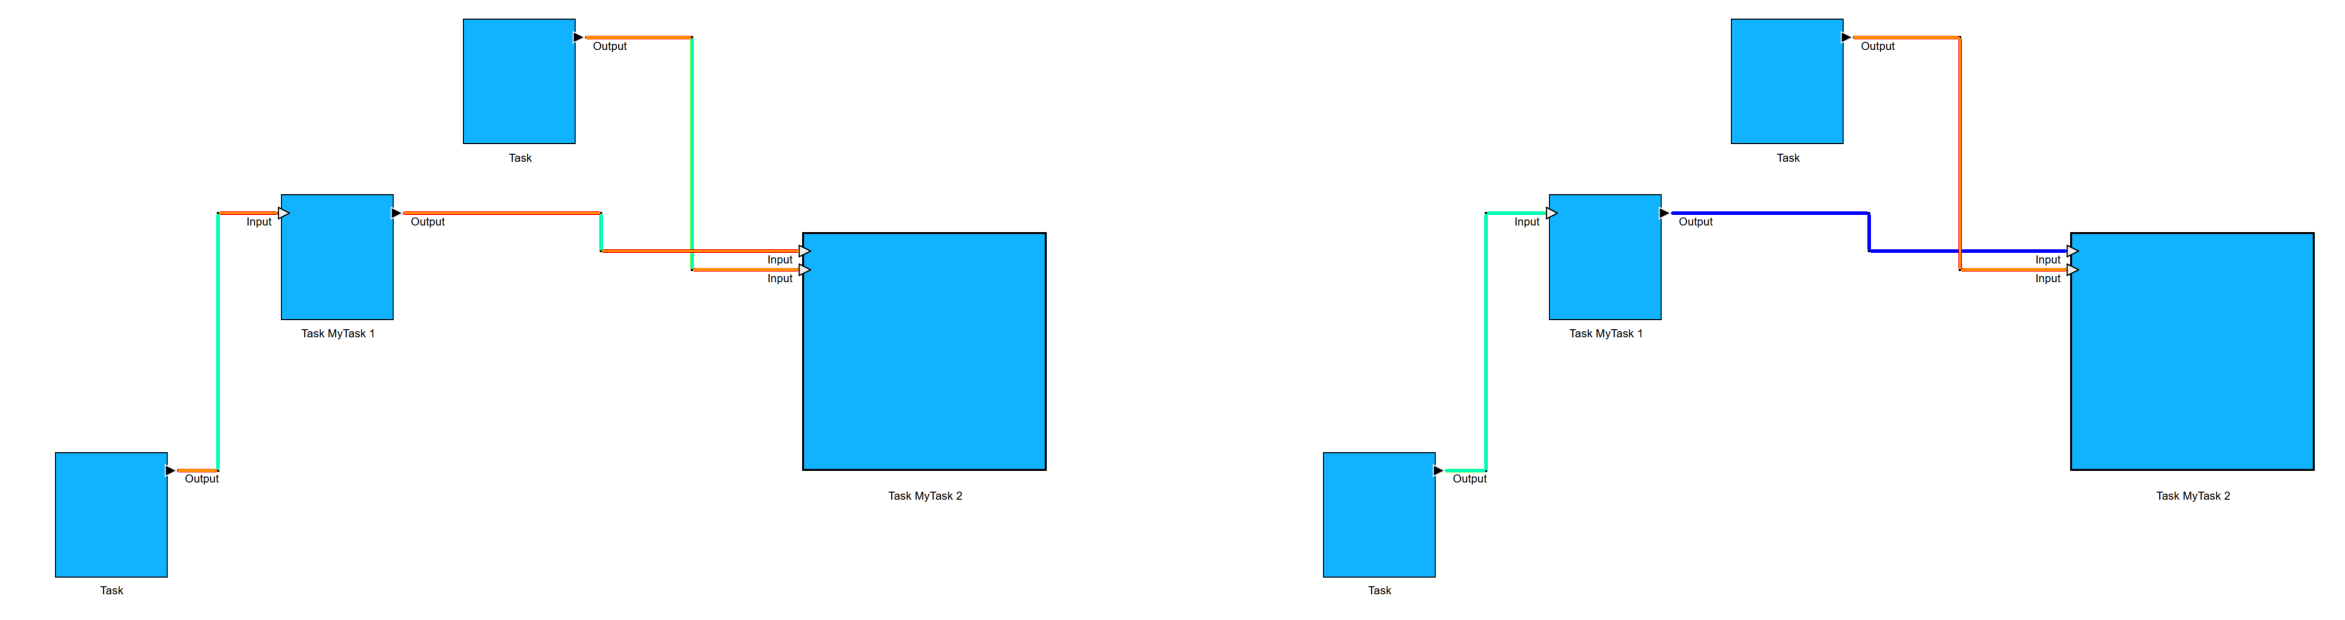
\includegraphics[width=\linewidth]{pictures/chains_before_after.png}
    \caption[Line segments being grouped into line segment chains]{Left: detected vertical and horizontal line segments. Colors distinguishing horizontal and vertical lines.\\Right: detected line segments grouped into individually colored line segment chains.}
    \label{fig:chains_before_after}
\end{figure}
Generating the polylines now would yield better results, but still create unusable data, because the line segments within each chain and the two points within each line segment are not sorted. The first point in a list of line segments in a chain could for example be a point in the middle of the chain, resulting in \acrshort{opencv}'s Polyline function to connect the following points in the wrong order.\\
The sorting algorithm for solving this problem consists of two steps: the first sorts the line segments from the beginning of the chain to the end, the second sorts the end- and startpoint of each line segment individually, so that they too appear in sequential order of 'flow' in the chain.\\
To distinguish between intermediate points and endpoints, the function relies on the method by which the points were initially identified: when two line segments intersect to form a 90\textdegree\ turn, each segment consists of a start- and an endpoint. As a result, intermediate points in a chain, where line segments meet, always have two points in close proximity, whereas endpoints only have a single point, since only one line segment terminates at each endpoint (see \autoref{fig:point_zoom}).
The method leverages this discrepancy by identifying endpoints through an iterative process: It examines each point and checks for the presence of other points within a seven-pixel radius. If no other points are found within this radius, the point is classified as an endpoint of a chain (see \autoref{lst:detecting_endpoints}).\\
\lstinputlisting[language=Python, firstline=40, lastline=47, caption={Differentiating between segment endpoints and intermediate points.}, label = {lst:detecting_endpoints}]{layout/code.m}
\begin{figure}
    \centering
    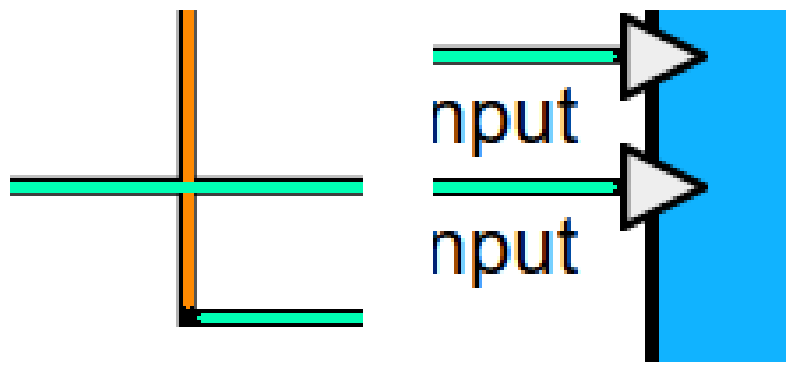
\includegraphics[width=0.5\linewidth]{pictures/zoomed_in_points.png}
    \caption[Intermediate points / Endpoints difference]{Intermediate points (left) have other points in close proximity, while endpoints (right) do not.}
    \label{fig:point_zoom}
\end{figure}
Using the identified endpoints to initialize the \textit{sorted\_chain} list allows the program to organize the chains systematically.\\
The process begins by selecting a segment that includes one of the start points as the initial segment of the chain. The endpoint of this segment that is not a chain endpoint is designated as the first \textit{last\_point} in the \textit{sorted\_chain} list. To determine the next segment in the chain, a \textit{lambda function} iterates through each remaining segment in the current chain, calculating the distance between the \textit{last\_point} and each point of each segment in the chain. The segment containing the point with the smallest distance to the \textit{last\_point} is selected as \textit{next\_segment} and removed from the list of \textit{remaining\_segments}. Within this segment, the point closest to the \textit{last\_point} is appended first to the \textit{sorted\_chain}, followed by the second point of the segment. This process repeats until no segments remain in the \textit{remaining\_segments} list. The entire process is repeated for each chain until all points in all chains are ordered according to the edge's \textit{flow} (see \autoref{lst:sorting_points}).
\lstinputlisting[language=Python, firstline=53, lastline=77, caption={Sorting each point in each chain according to the edges \textit{flow}}, label = {lst:sorting_points}]{layout/code.m}
\begin{figure}[h]
    \centering
    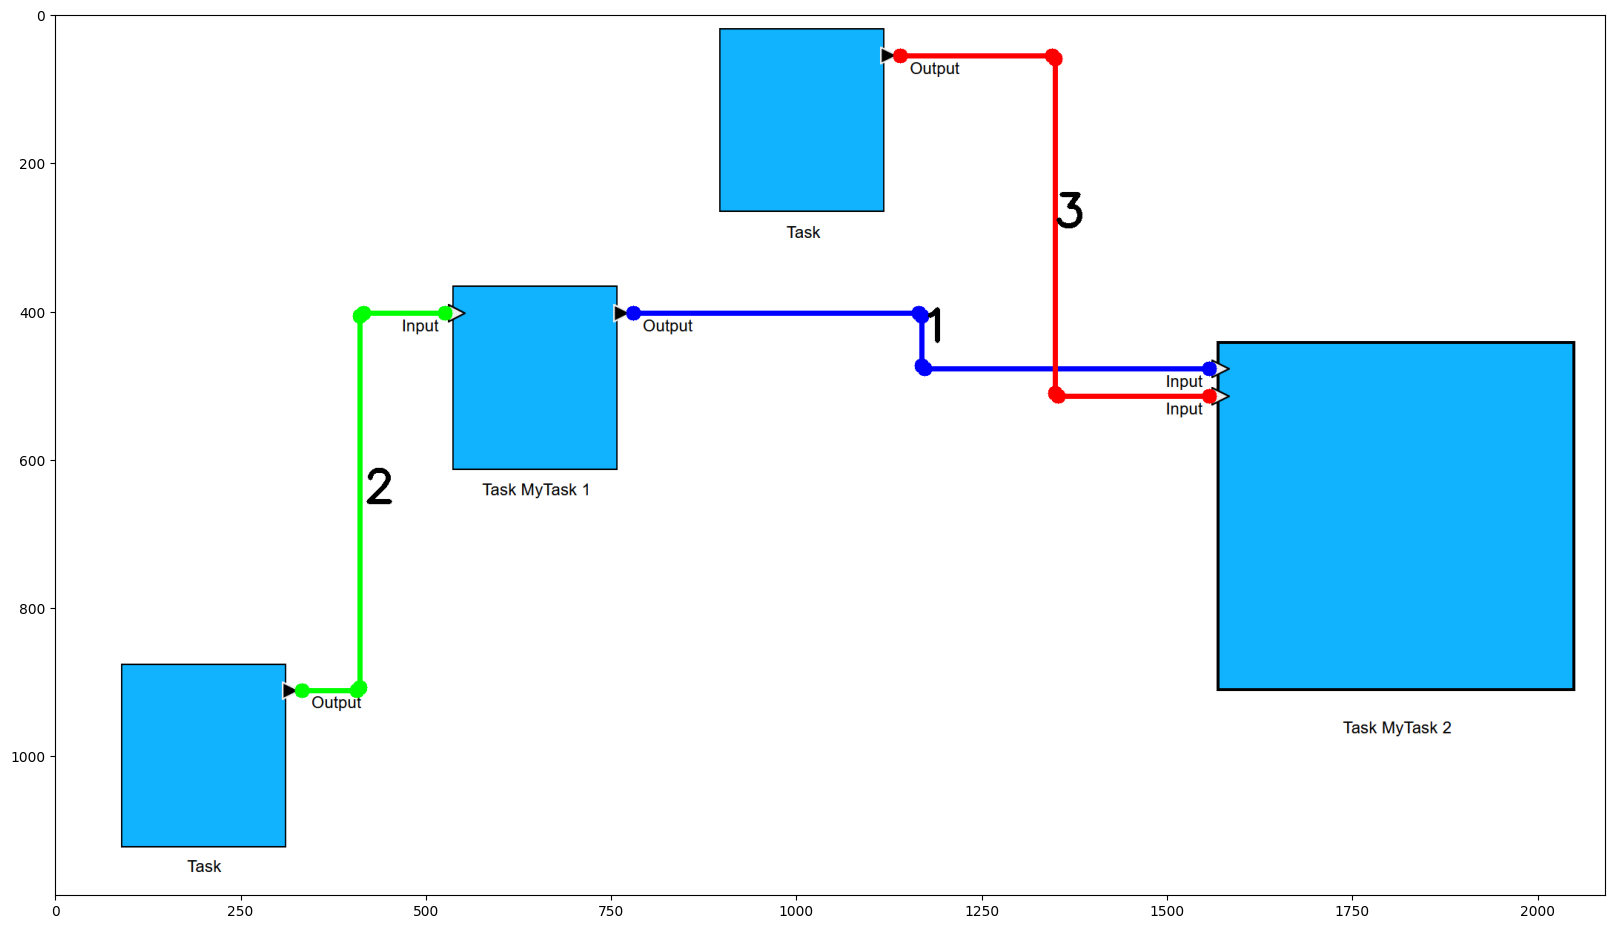
\includegraphics[width=0.7\linewidth]{pictures/polylines_found.png}
    \caption[Numbered polylines found in the functions editor]{Numbered polylines found in the functions editor. Connecting the points in the correct order results in the detected edges.}
    \label{fig:polylines_found}
\end{figure}
As seen in \autoref{fig:polylines_found}, the method successfully generates polylines from the initial screenshot. The order in which the polylines are initially detected depends on the order of the line segments and is not relevant for the final result.\\
Polylines, which represent connected line segments as ordered lists of points, are a fundamental component in reconstructing edges within the diagram. To generate these polylines from the sorted chains, the method iterates through the \textit{sorted\_chains} list, sequentially appending each point to construct the polylines. The preprocessing and sorting of the data ensures that the chains are already structured correctly, making the generation of polylines straightforward and efficient. Once the polyline is constructed, it is converted into the format required by \acrshort{opencv} for further processing.

\section{Vertex Detection}
\label{sec:vertex_detection}
Vertices represent distinct visual elements within \acrshort{xgee}, such as functions, devices, containers or \acrshort{io} ports. Identifying these vertices is critical for interpreting the structural arrangement of the diagrams. This section introduces a template-matching approach to address problems including overlapping vertices and varying sizes, ensuring a more reliable vertex detection in all considered diagram types within \acrshort{xgee}.

A major problem in template matching is the diversity of vertices within \acrshort{xgee}'s editor models. For example, the functions editor contains only functions, inputs and outputs, while the hardware editor contains devices and \acrshort{io} ports and the allocations editor contains devices, signal containers, signal arrows and subtasks which overlap with devices and contain their own set of \textit{sub-sub-vertices}. Additionally, some vertices are scalable, while others are not. Scalable vertices require extra processing to ensure accurate detection. However, applying this processing universally to all vertices would result in unpredictable and incorrect detections.

To address these challenges, the model is queried for a list of unique vertices. This list is analyzed to identify any vertices with the \textit{isSubVertexBody}-flag set, which indicates they are subvertices such as subtasks, that overlap with other vertices. These subvertices are prioritized and placed at the beginning of the list of vertices. This way, the vertex detection method can progressively simplify the image by erasing detected subvertices after the first iteration of the vertex detection function, allowing the underlying vertices to be detected without obstruction. Other relevant flags are:
\begin{itemize}
    \item \textit{isScalable} which indicates whether the vertex can be scaled
    \item \textit{sizeX} and \textit{sizeY} which specify the size of the vertex
    \item \textit{filepath} which specifies the path to the template image
    \item \textit{parent\_filepath} which specifies the path to the parent vertex in case it is a subvertex
\end{itemize}
The method iterates through the list of unique vertices in the current editor model, prioritizing subvertices identified in the previous step. These subvertices are removed from the image by setting all pixels within the bounding box of the subvertex to the \textit{fill} color of the parent vertex as shown in \autoref{fig:draw_boxes}. This process effectively removes the subvertices from the image, enabling the subsequent vertex detection steps to accurately identify the remaining vertices.\\
\begin{figure}[htb]
    \centering
    \begin{minipage}[b]{0.45\textwidth}
        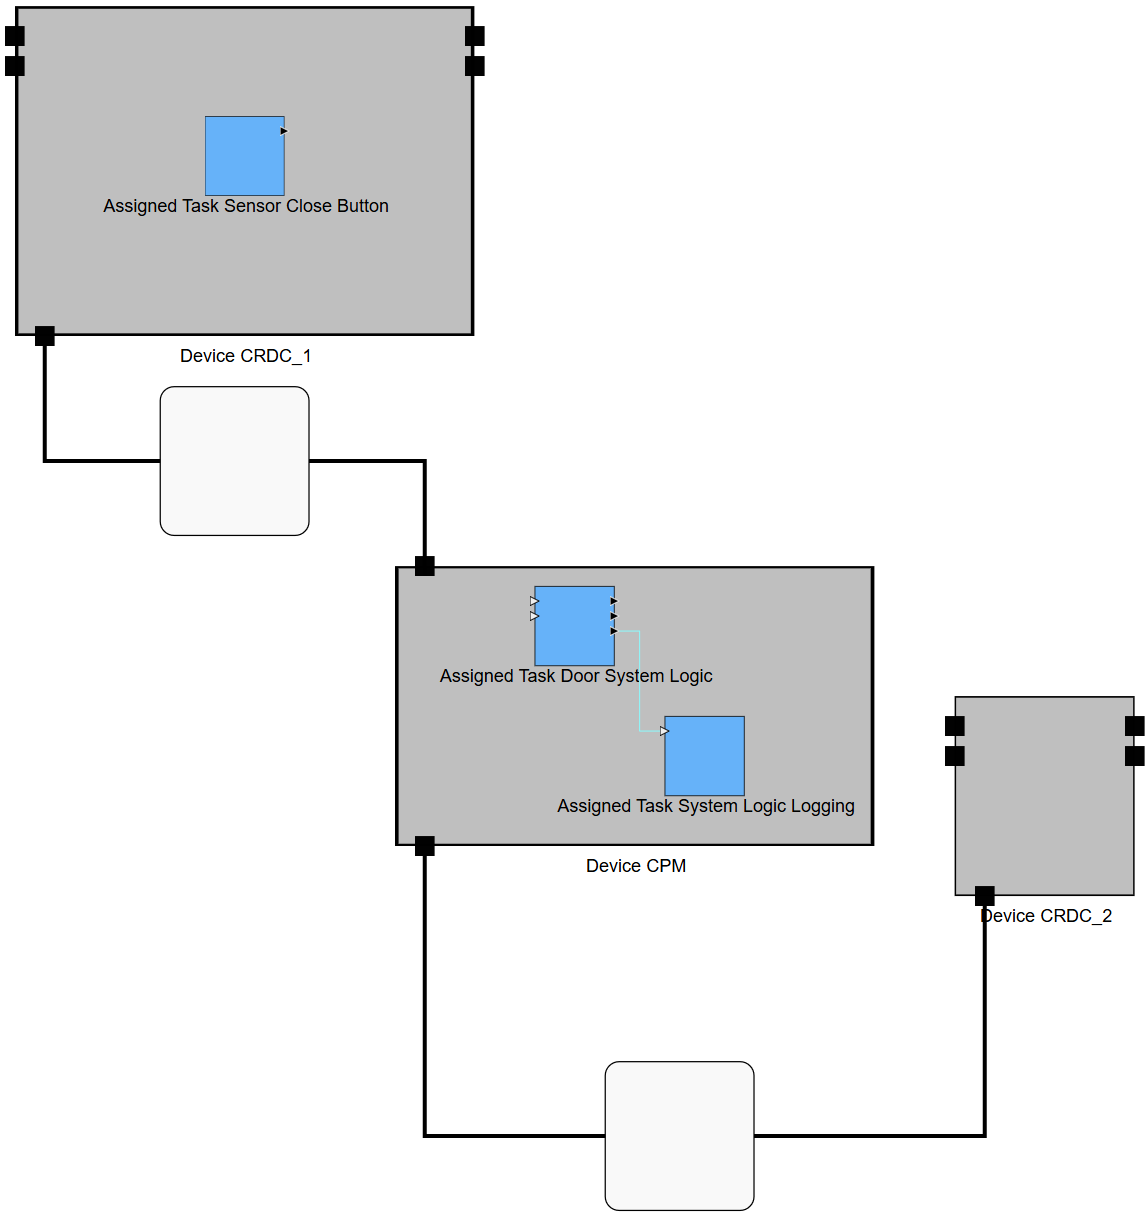
\includegraphics[width=\textwidth]{pictures/draw_boxes_before.png}
    \end{minipage}
    \hfill
    \begin{minipage}[b]{0.45\textwidth}
        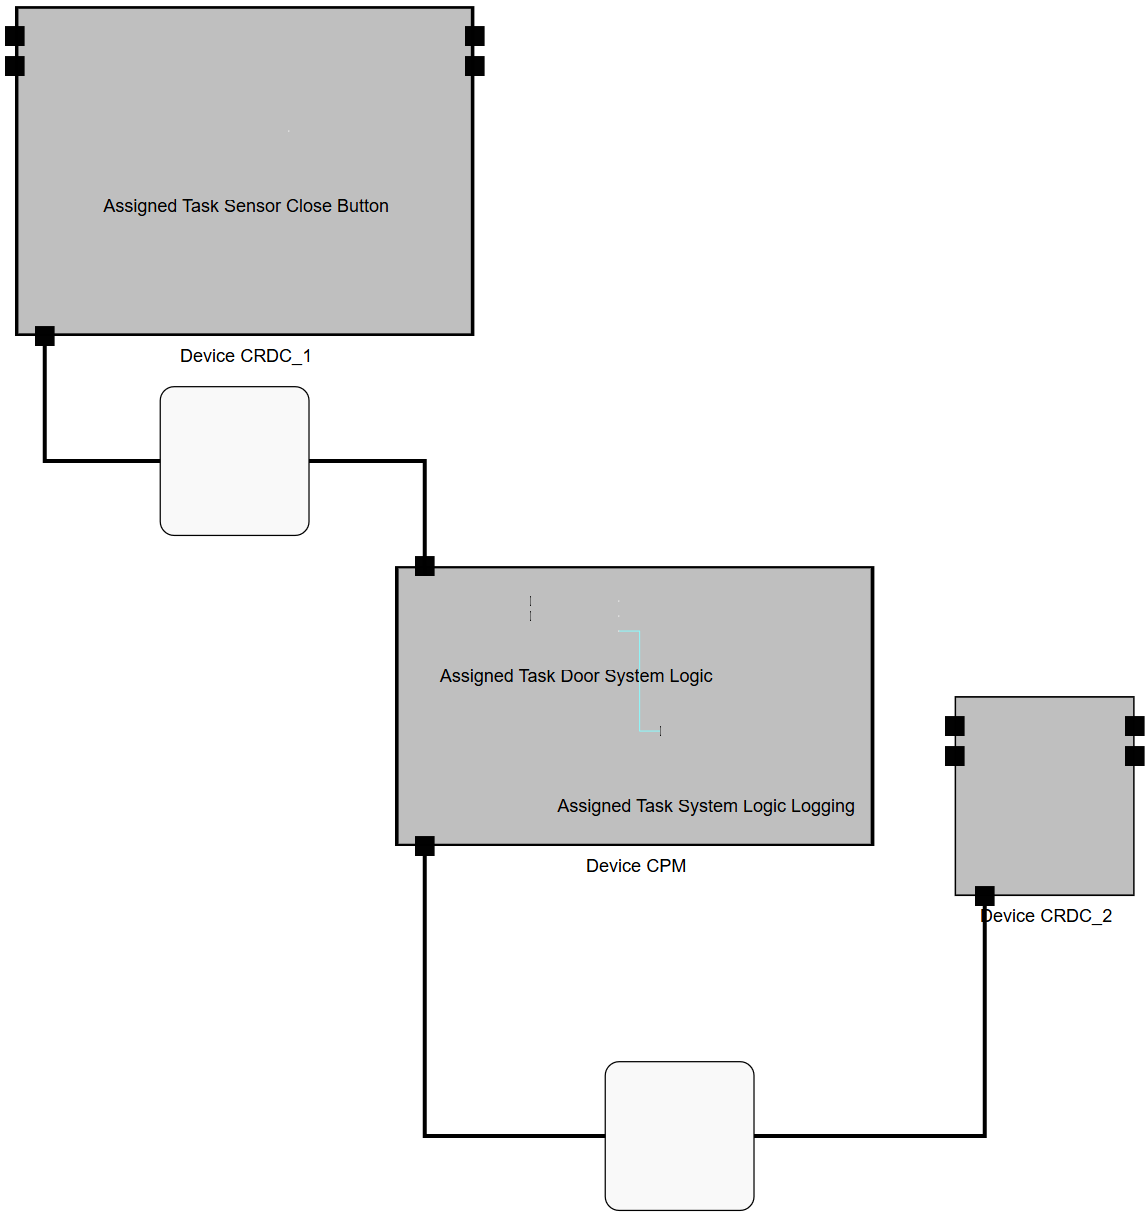
\includegraphics[width=\textwidth]{pictures/draw_boxes_after.png}
    \end{minipage}
    \caption[Automatic subvertex removal example]{Original image from allocations editor containing subvertices (left) and modified image with subvertices removed (right).}
    \label{fig:draw_boxes}
\end{figure}
After processing the subvertices, a new image object is created using the modified image. The method then iterates through the list of remaining vertices, loading the template image of each vertex using the \textit{filepath} attribute. Depending on the \textit{isScalable} flag, either the \textit{ScalableVertexDetector} or one of the \textit{UnscalableVertexDetector}s is initiated and the corresponding vertex detection is applied.\\
In case of unscalable vertices, \acrshort{opencv}'s \textit{matchTemplate} and \textit{normalize} functions are applied. The resulting data is thresholded to identify the positions of all found vertices. To define the vertex boundaries, the \textit{sizeX} and \textit{sizeY} attributes are used, allowing bounding boxes of the correct size to be drawn with the detected match serving as the upper-left corner. This approach is effective for detecting vertices like \acrshort{io} ports and subtasks.\\
In case of scalable vertices, this approach does not work because the size of the vertex is variable, which reduces the certainty of found matches drastically and eliminates constant \textit{sizeX} and \textit{sizeY} values as a reliable method for defining bounding boxes.\\

Scalable vertices within \acrshort{xgee} are function- and device containers that can be resized to improve the readability of visualizations. However, the initial scalable vertex detection algorithm often produced inaccurate results when applied to large function- and device containers. Specifically, it tended to produce higher similarity scores at the corners of the container, as the black border surrounding the vertex at these locations more closely resembled the black border in the template image. In contrast, the absence of a black border in the center of the container led to lower similarity scores. In extreme cases, this resulted in the center of the vertex not being detected at all, with the algorithm instead falsely identifying four smaller vertices at the container's corners. The same issue occurred with large devices.\\
To detect these vertices regardless of their dimensions, multiple templates of the same size for different parts of the large vertex as illustrated in \autoref{fig:templates} are required. They are generated from the (leftmost) original template image by cropping its edges and corners in different ways.
\begin{figure}[ht]
    \centering
    
\includegraphics[width=0.85\linewidth]{pictures/templates.png}
    \caption[Template matching template generation]{Templates for scalable vertex detection generated from the original (leftmost) template image, black edges are exagerated for clarity.}
    \label{fig:templates}
\end{figure}
Template matching is performed iteratively with each template, comparing the results after each iteration. The highest similarity score for each pixel is retained and combined into the resulting data, which is then thresholded to extract all potential matches.\\
Typically, numerous matches are identified during this process. To eliminate false positives and process the matches to determine the differently sized bounding boxes of the vertices, the algorithm described by Andreas Waldvogel and Bj{\"o}rn Annigh{\"o}fer in \cite{waldvogel_annighoefer_models_2024} is applied.\\
The original image is thresholded to distinguish foreground from background pixels, as illustrated in \autoref{fig:foreground_threshold}. This foreground information is then utilized to filter the detected matches, retaining only those located within the foreground area. This process effectively removes false positives which often occur because the black pixels along the edges and borders of function or device containers closely resemble those in the black borders in the template images.
\begin{figure}[htb]
    \centering
    \begin{minipage}[b]{0.36\textwidth}
        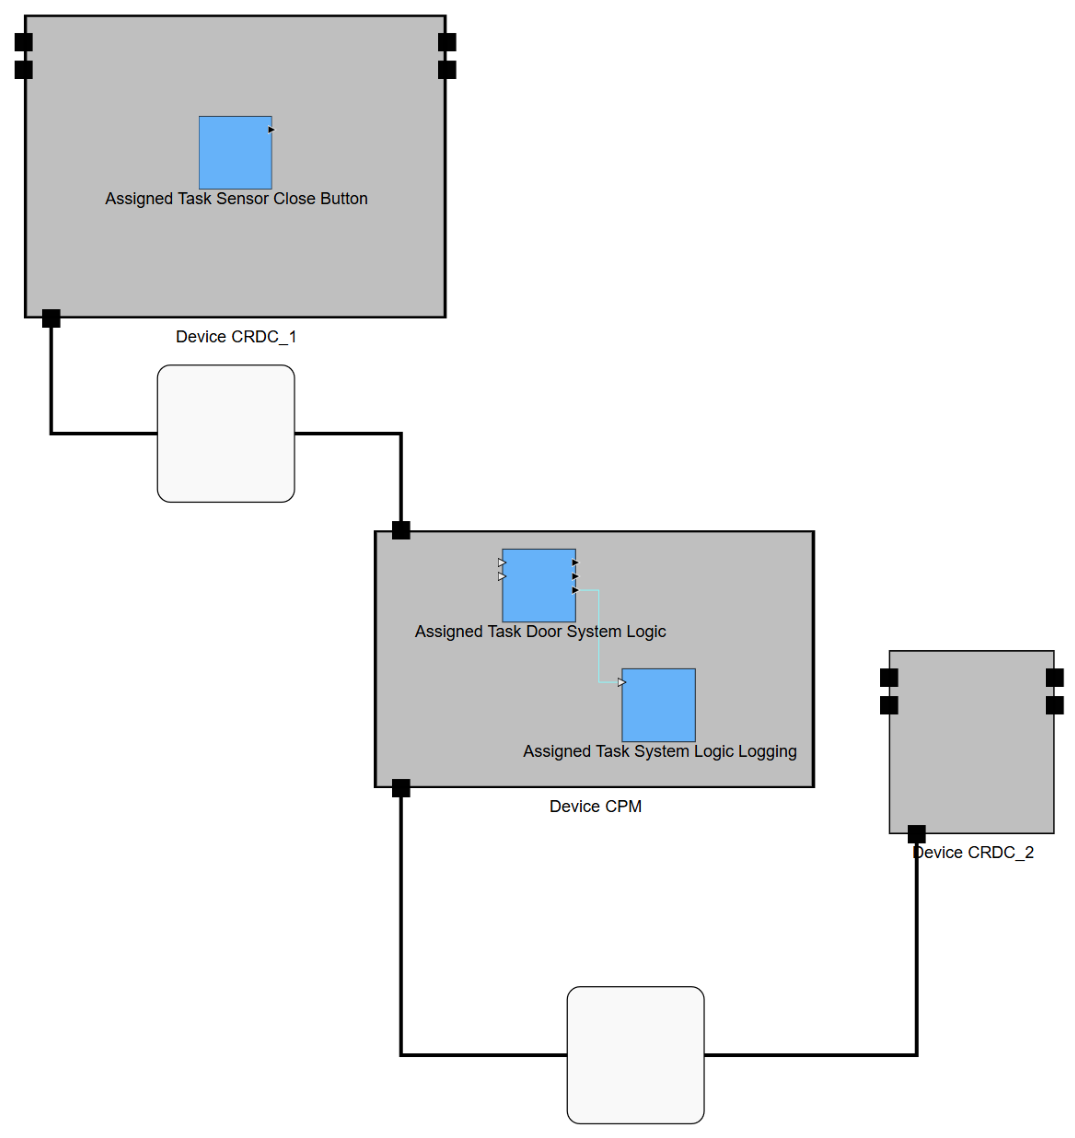
\includegraphics[width=\textwidth]{pictures/foreground_threshold_before.png}
    \end{minipage}
    \hfill
    \begin{minipage}[b]{0.36\textwidth}
        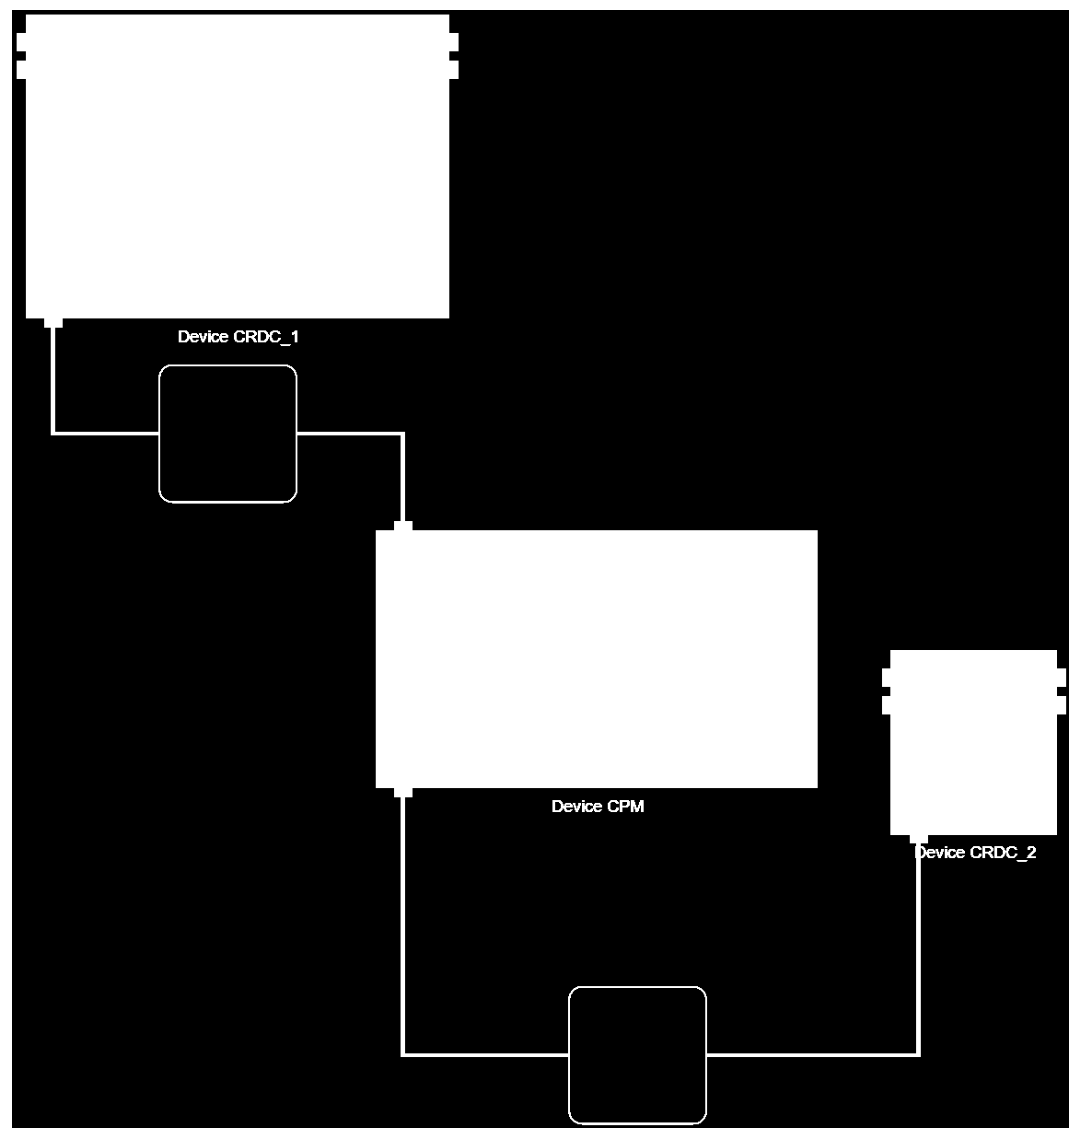
\includegraphics[width=\textwidth]{pictures/foreground_threshold_after.png}
    \end{minipage}
    \caption[Extraction of foreground pixels]{The allocations editor screenshot (left) is thresholded to extract the foreground pixels (right).}
    \label{fig:foreground_threshold}
\end{figure}\\
For each remaining detected match, the \textit{sizeX} and \textit{sizeY} attributes are used to create a filled bounding box around the detected position. Since multiple matches are often found at various locations within a single large vertex, the overlapping bounding boxes collectively form a larger structure. This structure is then simplified into a single bounding box using \acrshort{opencv}'s \textit{findContours} function.
\begin{figure}[htb]
    \centering
    \begin{minipage}[b]{0.36\textwidth}
        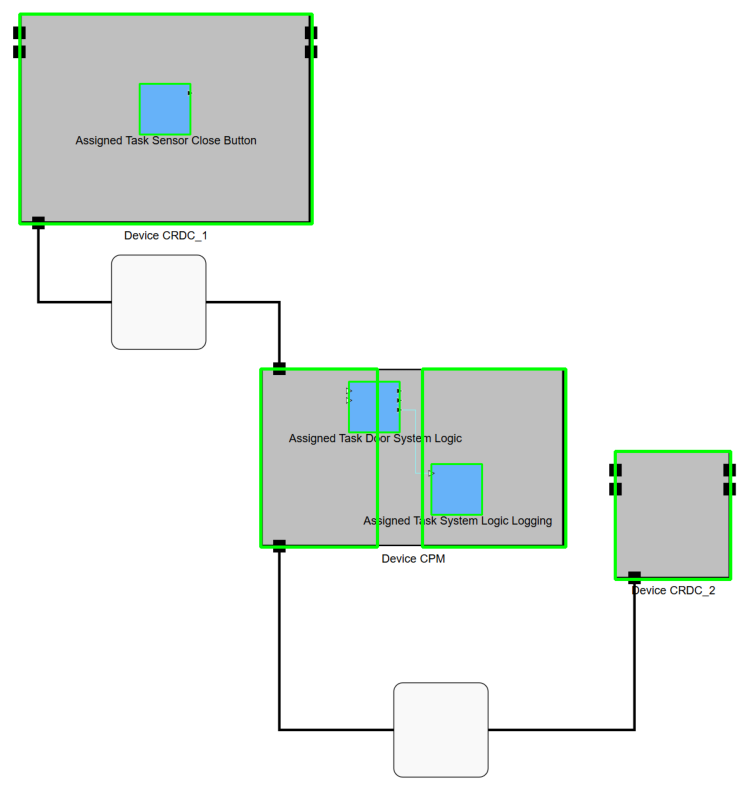
\includegraphics[width=\textwidth]{pictures/many_templates_before.png}
    \end{minipage}
    \hfill
    \begin{minipage}[b]{0.36\textwidth}
        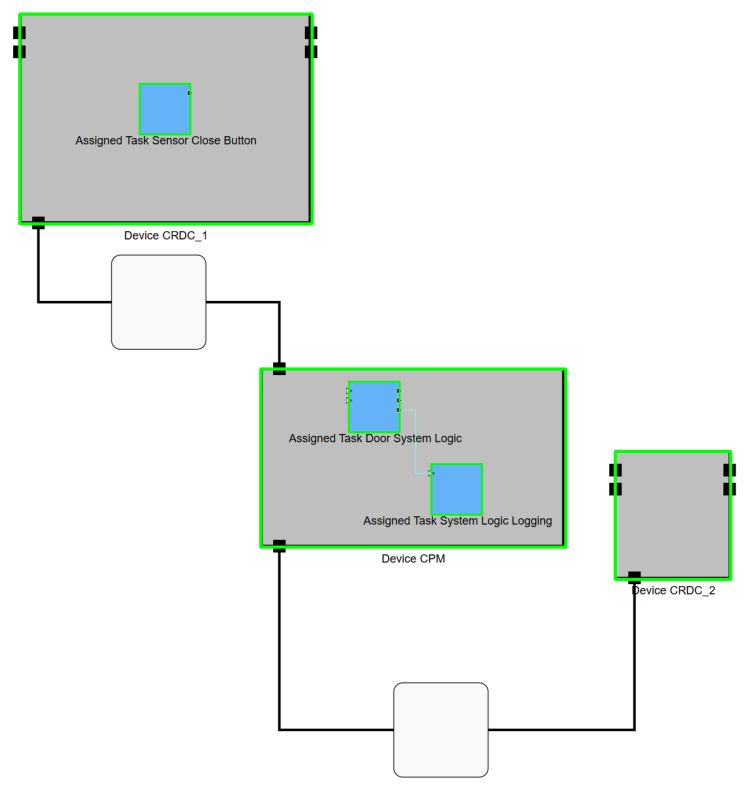
\includegraphics[width=\textwidth]{pictures/many_templates_after.png}
    \end{minipage}
    \caption[Complete detection of very large devices]{Image from allocations editor containing a large, partially detected device using one template(left) and containing a large, fully detected device using multiple templates(right).}
    \label{fig:many_templates}
\end{figure}
This approach successfully detects all scalable vertices within \acrshort{xgee} regardless of their dimensions. Using both scalable and non-scalable vertex detection methods ensures that all vertices are accurately identified.\\
\autoref{fig:many_templates} illustrates the original method's difficulties when dealing with large vertices with overlapping subvertices. On the left, in the center portion of the device, no matches are found due to the absence of black borders and interference with the remaining text of the subtasks. On the right, many templates are used to detect the entire device, resulting in a more accurate detection.\\
The method is capable of detecting all vertices in the 20 unique test cases within this paper, including subvertices and scalable vertices.

\section{Text Recognition}
\label{sec:text_recognition}
The original text detection in \acrshort{xgee} utilized Pytesseract \cite{pytesseract_2024}, an open-source \acrlong{ocr} (\acrshort{ocr}) engine developed and sponsored by Google in 2006. Pytesseract required separate installation from other packages and could only detect text in images that had been preprocessed. Additionally, the output data required extensive postprocessing to become usable. While Pytesseract demonstrated high accuracy and speed, it struggled to reliably detect small text or text with low contrast to the background. Its optimization for structured text formats, such as those found in books, further hindered its performance in \acrshort{xgee}, where text can appear in varying orientations, sizes, and positions. These limitations made reliable text detection using Pytesseract difficult to achieve.

\begin{figure}[htb]
    \centering
    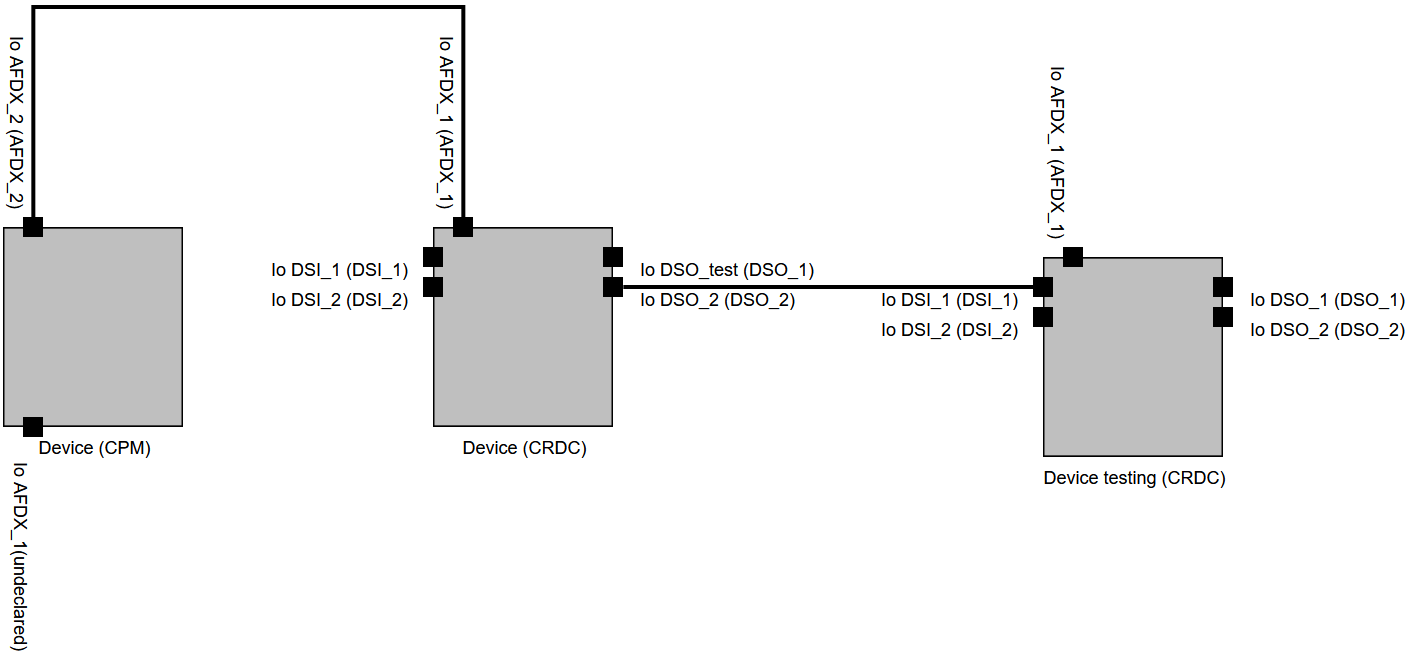
\includegraphics[width=0.8\linewidth]{pictures/text_before.png}
    \caption[Text detection of rotated text before]{Input image from hardware editor containing rotated text}
    \label{fig:text_before}

    \centering
    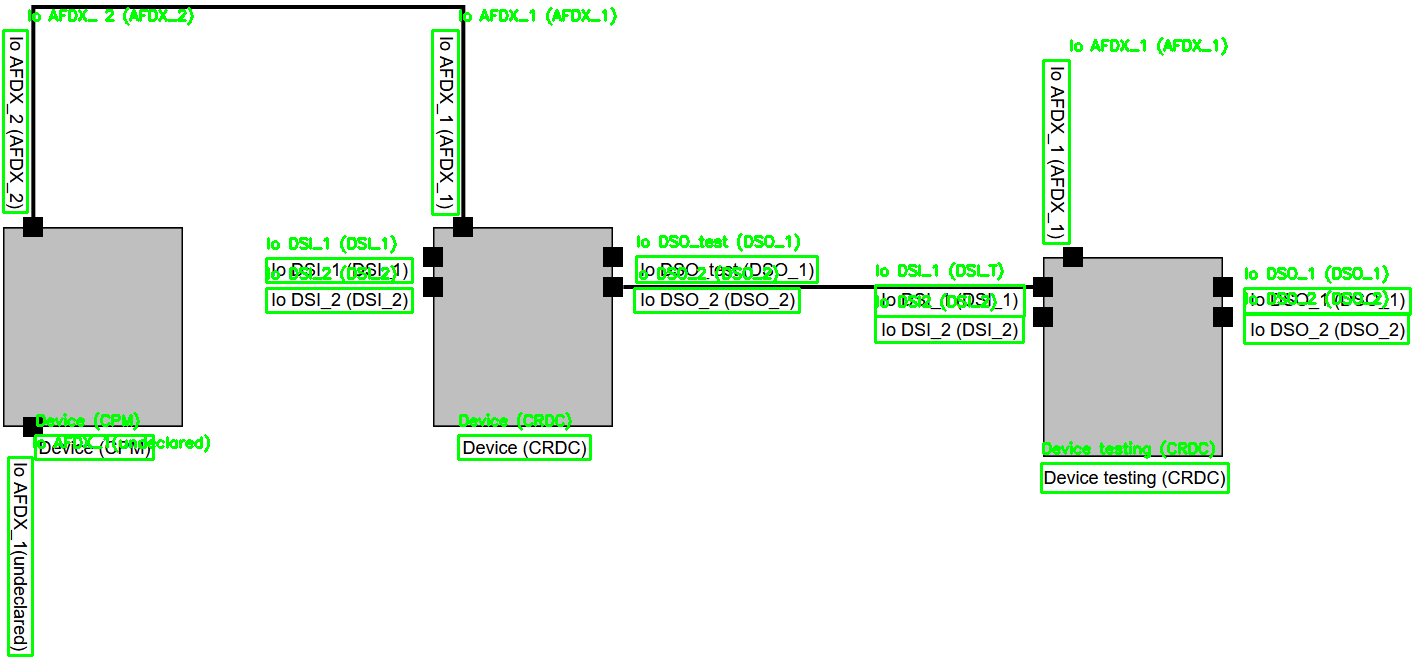
\includegraphics[width=0.8\linewidth]{pictures/text_after.png}
    \caption[Text detection of rotated text after]{Output image from hardware editor containing text bounding boxes}
    \label{fig:text_after}
\end{figure}
After evaluating various \acrshort{ocr} engines, including Easy\acrshort{ocr} \cite{easyocr_2024}, Doctr \cite{doctr_2024}, and Keras-\acrshort{ocr} \cite{keras_ocr_2023}, Easy\acrshort{ocr} proved to be the most suitable alternative.\\
Easy\acrshort{ocr} is a deep-learning-based \acrshort{ocr} engine that reliably detects text in images, even under challenging conditions such as low contrast or resolution. Although it operates more slowly on modern \acrshort{cpu}s compared to some alternatives, it performs significantly faster on \acrshort{gpu}s. Additionally, its ability to detect text in multiple languages adds potential value for future applications. Integration of Easy\acrshort{ocr} into the \acrshort{xgee} editor for the user is straightforward, as it can be installed directly via \textit{pip install} easy\acrshort{ocr} through the requirements.txt file without requiring additional dependencies or downloads. Unlike Pytesseract, Easy\acrshort{ocr} only necessitates minimal image preprocessing, and it structures found characters into words and sentences automatically based on proximity, eliminating the need for extensive postprocessing. These advantages make Easy\acrshort{ocr} the optimal choice for the updated text detection pipeline within \acrshort{xgee}.

First, a reader object is created and the language of the text is specified. The readtext function of the reader object is then called with the image as an argument. The image has to be padded to have a square shape, so it can be easily rotated. To ensure a more reliable detection, the image is slightly blurred and upscaled to counter any aliasing and small characters. The text detection function then returns a list containing the detected text, its bounding box, and a certainty factor. Parameters can be specified when calling this function to adjust the expected text properties, enhancing the reliability of the detection. For example in earlier versions, Easy\acrshort{ocr} struggled to detect single numbers, likely because its language model has been trained on data not containing any single characters, but with these parameter adjustments, the occurance of this issue has been reduced.\\
The detection process is repeated for the rotated version of the image to detect rotated text labels, present in the hardware layer, as well. The positions of the bounding boxes of the found rotated text are then rotated around the center of the image to reallign them with the found text of the original image. The found bounding boxes and text are illustrated in \autoref{fig:text_before} and \ref{fig:text_after}. Reading an image which contains rotated text usually results in many falsely read characters, because for example 'o' and 'l' can be interpreted regardless of orientation. To filter out the falsely read characters, the algorithm first combines the found results of both \acrshort{ocr}-searches and then removes every word shorter than three letters.\\
\begin{figure}[H]
    \centering
    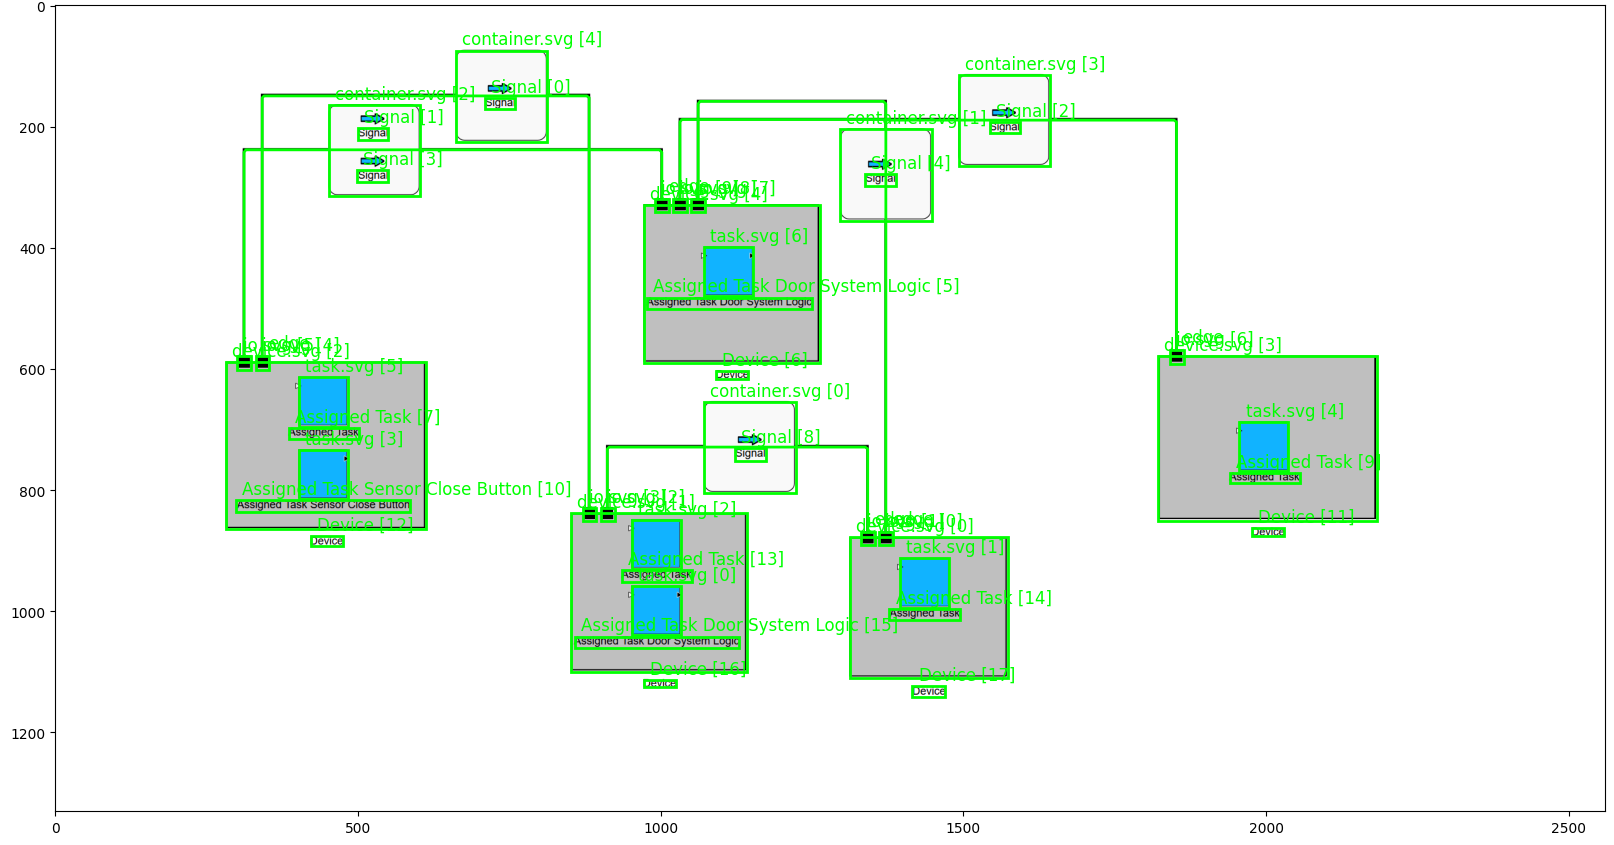
\includegraphics[width=0.85\textwidth]{pictures/allocations_found_tokens.png}
    \caption[Debugging image of bounding boxes and token names]{Debugging image of bounding boxes and token names found during the tokenization of the allocations layer, demonstrating the capability of the tokenization pipeline.}
    \label{fig:allocations_found_tokens}
\end{figure}
Because easy\acrshort{ocr} automatically groups detected characters into words and sentences, this is a simple and effective method to filter out falsely read characters. Using this approach also allows the same algorithm to be used for all models, regardless of the \acrshort{xgee} editor they were created in, simplifying the integration into the \acrshort{xgee} codebase.
In conclusion, these methods enhance the tokenization process compared to the previous implementation. As seen in \autoref{fig:allocations_found_tokens}, the combined methods are able to correctly identify all token types in the allocations editor, utilizing all previously mentioned methods.\\
The new edge detection identifies edges regardless of length and orientation. Intersections and signal containers are correctly identified and processed, ensuring that all detected edges are continuous. The vertex detection method is capable of detecting scalable vertices of varying sizes, unscalable vertices, \acrshort{io} ports, and subtasks, even when they overlap. The text detection method is capable of detecting text in varying orientations and positions. The combined methods provide a robust and reliable tokenization pipeline for \acrshort{xgee}, capable of accurately identifying all relevant tokens in the editor models.\footnote{The described methods can be found individually at \url{https://github.com/franzbanz/computervision}\\and implemented into \acrshort{xgee} at \url{https://gitlab.com/xgee/xgee-example-app}.}
\chapter{Integration}
\label{chap:Integration}
This chapter provides an in-depth explanation of how the described methods were implemented into the larger \acrshort{xgee} codebase.

\section{System Overview and Workflow}
\label{sec:system_overview}

\acrshort{xgee} is a web-based graphical model editor that utilizes an editor model to define editors for ecore models in a model-driven approach, enabling visualization and interaction. The editor model supports the model-driven definition of editors for ecore models, incorporating both visualization and interaction \cite{waldvogel_annighoefer_models_2024}.

\acrshort{xgee}'s visualization verification is implemented as a modification to the main editor, mostly within the \textit{detector.py} and \textit{diagram\_tokenization\_orchestrator.py} files.
For the verification process to function correctly, a screenshot of the entire screen is preprocessed to isolate the relevant portions of \acrshort{xgee}'s editor window by removing elements like the browser \acrshort{ui} and background grid. During the tokenization step, the positions, dimensions and contents of edges, vertices, and text are detected and stored. This data is subsequently used in the syntactical analysis to identify inconsistencies in parent-child relationships between tokens. (Syntax in this context means the positioning rules of vertices, edges and text labels defined in the editor model.)\\
A new model is then instantiated based on the detected tokens and the visualization model. This model is compared to the original and any discrepancies are highlighted through both graphical and textual user interfaces.\\
Edge, vertex, and text detections occur during the tokenization phase of the verification pipeline. In the original integration, each detection algorithm was implemented as a class within the \textit{detector.py} file, while their execution was managed by the \textit{diagram\_tokenization\_orchestrator.py} file, which determined the order and process of the tokenization. This structure is retained and extended in the new implementation.

\section{Edge Detection Integration}
The integration of the new edge detection algorithm into \acrshort{xgee} is simplified by its use of the already existing interface for inputs and outputs. This approach ensures that the system remains modular and scalable.\\
To implement the new functionality, the algorithm is divided into sections, each expressed as an individual function in the code. These functions are appended to the edge detection class, maintaining modularity and readability. By ensuring the edge detection operates with the same input (screenshots) and provides the same output (\acrshort{opencv} polylines) as the original method, the new implementation can be integrated without requiring large changes to the existing codebase.\\
The \textit{diagram\_tokenization\_orchestrator} queries information such as the stroke width and color from the editor model, which could be used in the future to further generalize the edge detection. It also instantiates an object of the edge detection class, passing the workspace path as an argument to extract data like the intersection template. The polylines are stored using a dedicated data storage function, ensuring subsequent steps proceed smoothly without requiering additional integration effort. 

\section{Vertex Detection Integration}
The integration of a new vertex detection algorithm into \acrshort{xgee}'s codebase required addressing problems such as order-dependent method execution and enabling functions to dynamically share and modify input data at runtime.\\
Previously, a list of vertices for the current editor, generated by the \textit{diagram\_tokenization\_orchestrator}, drove the vertex detection process. The method iterated through this list, performing detection cycles for each vertex type, distinguishing between scalable and non-scalable vertices. However, this static approach proved inadequate in the allocations editor due to overlapping vertices, where detecting the top-level vertex first becomes critical. Furthermore, it was not possible for functions to pass intermediate results, such as detected subtasks, to subsequent functions. This was because the input (a preprocessed screenshot) was initialized at the start of the verification process using the \textit{ImageWrapper} class and remained static throughout.\\
To solve these issues, the new implementation preprocesses the list of editor vertices to ensure vertex detection in the correct hierarchical order and introduces a way for input images to be updated dynamically during runtime.

In the new implementation, the \textit{diagram\_tokenization\_orchestrator} queries vertex attributes such as the filepath, shape, positioning within other vertices and the parent's filepath from the editor model domain. The vertex's position within the list of editor vertices is determined by the presence of the \textit{isPositioningBody} attribute: vertices with this attribute are classified as subvertices, while those without it are considered top-level vertices. Subvertices need to be detected first, as their overlap with parent vertices would otherwise interfere with the reliable detection of those parent vertices.\\
Using these attributes, the list of editor vertices is first sorted, prioritizing subtasks. The \textit{diagram\_tokenization\_orchestrator} then iterates through the sorted list, performing vertex detection for each vertex type. 
To enable the vertex detection function to alter the input of all subsequent iterations of the function, the creation of the \textit{ImageWrapper} object is shifted inside the vertex detection loop. This enables a new \textit{ImageWrapper} Object to be instantiated for every iteration, using the updated image.\\
For subvertices, a new function overlays the detected bounding boxes in the target image with the parent vertex's main color (e.g. the gray of device vertices is used to erase the top-level subtasks). The altered image is then used to instantiate the ImageWrapper, ensuring subsequent stages of vertex detection and verification operate on the updated input. This iterative approach enables precise detection of both subvertices and their parent vertices while simplifying the image progressively.
After all subvertices are processed, almost all remaining vertices can be detected using the methods described in \autoref{sec:vertex_detection}, as the subvertices no longer interfere with the detection process.\\
An alternative approach for resolving overlapping vertices described in \autoref{sec:edge_detection} has been implemented for signal container detection in the allocations editor, facilitating the need to process signal containers seperately using a distinct detection class and seperating them from the other vertices using the \textit{filepath} attribute.\\
Because container vertices are non-scalable, the newly created \textit{ContainerDetector} class inherits from the existing \textit{PortDetector} class (see \autoref{fig:inheritance_diagram}). This inheritance allows the \textit{ContainerDetector} to reutilize the majority of the functionality provided by \textit{PortDetector}, while overriding the \textit{detect\_vertices} function to implement a specialized detection process tailored to container vertices.
\begin{figure}
    \centering
    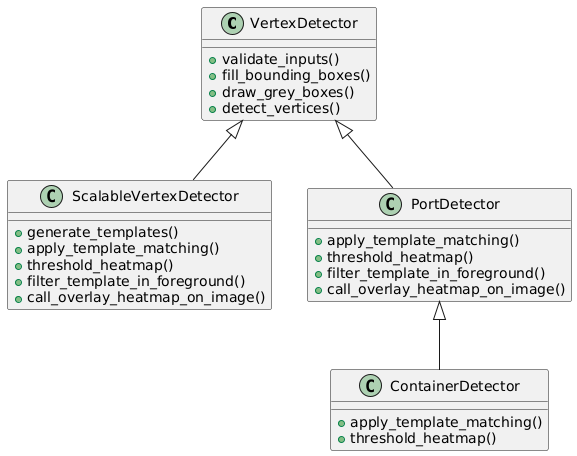
\includegraphics[width=0.5\textwidth]{pictures/inheritance_diagram.png}
    \caption[Inheritance diagram]{Inheritance diagram of the vertex detection classes created using \textit{PlantUML} \autocite{plantuml_2024}. The \textit{ContainerDetector} class inherits from the \textit{PortDetector} class, allowing it to reuse the majority of the functionality provided by \textit{PortDetector}.}
    \label{fig:inheritance_diagram}
\end{figure}
Depending on the vertex type, an object of either \textit{ScalableVertexDetector}, \textit{ContainerDetector} or \textit{PortDetector} is instantiated and used to detect the vertices.\\
The detected vertices are stored using a dedicated data storage function, ensuring subsequent steps proceed smoothly without requiring additional integration effort.

\section{Text Recognition Integration}
The integration of Easy\acrshort{ocr} into the \acrshort{xgee} codebase is achieved by utilizing the Easy\acrshort{ocr} \acrshort{api} within \textit{diagram\_tokenization\_orchestrator.py}. The \textit{detect\_text} function is updated to employ Easy\acrshort{ocr} for text extraction from preprocessed images. The extracted text is then stored using the existing dedicated data storage function, ensuring compatibility with subsequent processing steps.
Unlike PyTesseract, Easy\acrshort{ocr} includes inconsistent padding around detected text regions, resulting in less precise positional data. This discrepancy caused inconsistencies in positional accuracy and introduced errors in downstream model comparison methods. To ensure compatibility with the already existing interface, the dimensions of the bounding boxes were adjusted to more closely match those of PyTesseract. A positioning margin was implemented as well to reduce the need for bounding boxes to be positioned pixel-perfectly, reducing the amount of interfering error indications.

\section{Testing and Validation of the Integration}
To test the methods, the \acrshort{xgee} editor is used to create models with a known structure, incorporating different test cases in different editor layers. The model is processed by the verification pipeline. If necessary, text, vertex, or edge detections can be turned off to accelerate testing and reduce the workload when evaluating newly implemented methods. The results are compared to the expected output, and any discrepancies are analyzed to identify the cause. To further streamline the testing process, all previously mentioned methods log intermediate images and results using a dedicated Python logging package. This simplifies the process of identifying and resolving new issues.

To classify the performance of all newly implemented methods, 20 unique testcases in each editor model were processed and analyzed to demonstrate the functionality and limitations of the new additions. These evaluations are presented in \autoref{chap:evaluation}.
\chapter{Results}
\label{chap:evaluation}

To evaluate the newly implemented functionality, a series of test cases are used. These test cases are created by directly manipulating the model's vector graphics using the \textit{Firefox Developer Tools}. Individual vertices can be manipulated directly within the browser by decoding a \textit{base64}-encoded string that represents the graphic into a readable format that describes the properties of the corresponding \textit{.svg} file. Adjustments to attributes such as \textit{fill} followed by re-encoding the data into \textit{base64} allows changing the appearance of the visualization. Similarly, vertex positions can be modified, or vertices can be removed entirely, by adjusting the relevant values within the developer tools.\\
All test cases are derived from the models shown in \autoref{fig:unaltered_layers} and are simulated with minimal deviations to ensure accuracy.

\section{Test Cases}
\label{sec:test_cases}
Because the Error indications differ based on the step of the pipeline the error was found in, the testcases are divided into three categories:
\begin{itemize}
    \item Testcases where the error can be indicated textually as well as visually highlighted inside the editor (see \autoref{tab:test_cases}).
    \item Testcases where the error can only be indicated via a textual error indication (see \autoref{tab:test_cases_text}).
    \item Testcases without any simulated errors to illustrate the pipeline's capability to deal with complex models (see \autoref{tab:functional_test_cases_no_errors}).
\end{itemize}
\autoref{tab:test_cases} shows the results of testcases where the error can be identified and visually highlighted inside the \acrshort{xgee} Editor, as well as indicated via the textual log. The first column in \autoref{tab:test_cases} provides a brief description of the simulated error and the used error model. The second column provides an image of the relevant portion of the screenshot with the error highlighted. If the error type is found to be \textit{Untokenized Pixels}, the highlighting color is purple, otherwise, the color is red. The third column provides the textual error indication alongside the step of the verification pipeline, where the error was detected. In some cases, for example when a device with multiple \acrshort{io}s is removed or too small to be detected, many error indications of the same type are generated. In this case, only a few of the error indications are shown in the table and further errors of the same type are indicated using `` $\lowvdots$\ ''.

\begin{figure}[htb]  \centering
    \begin{minipage}{0.4\textwidth}
        \centering
        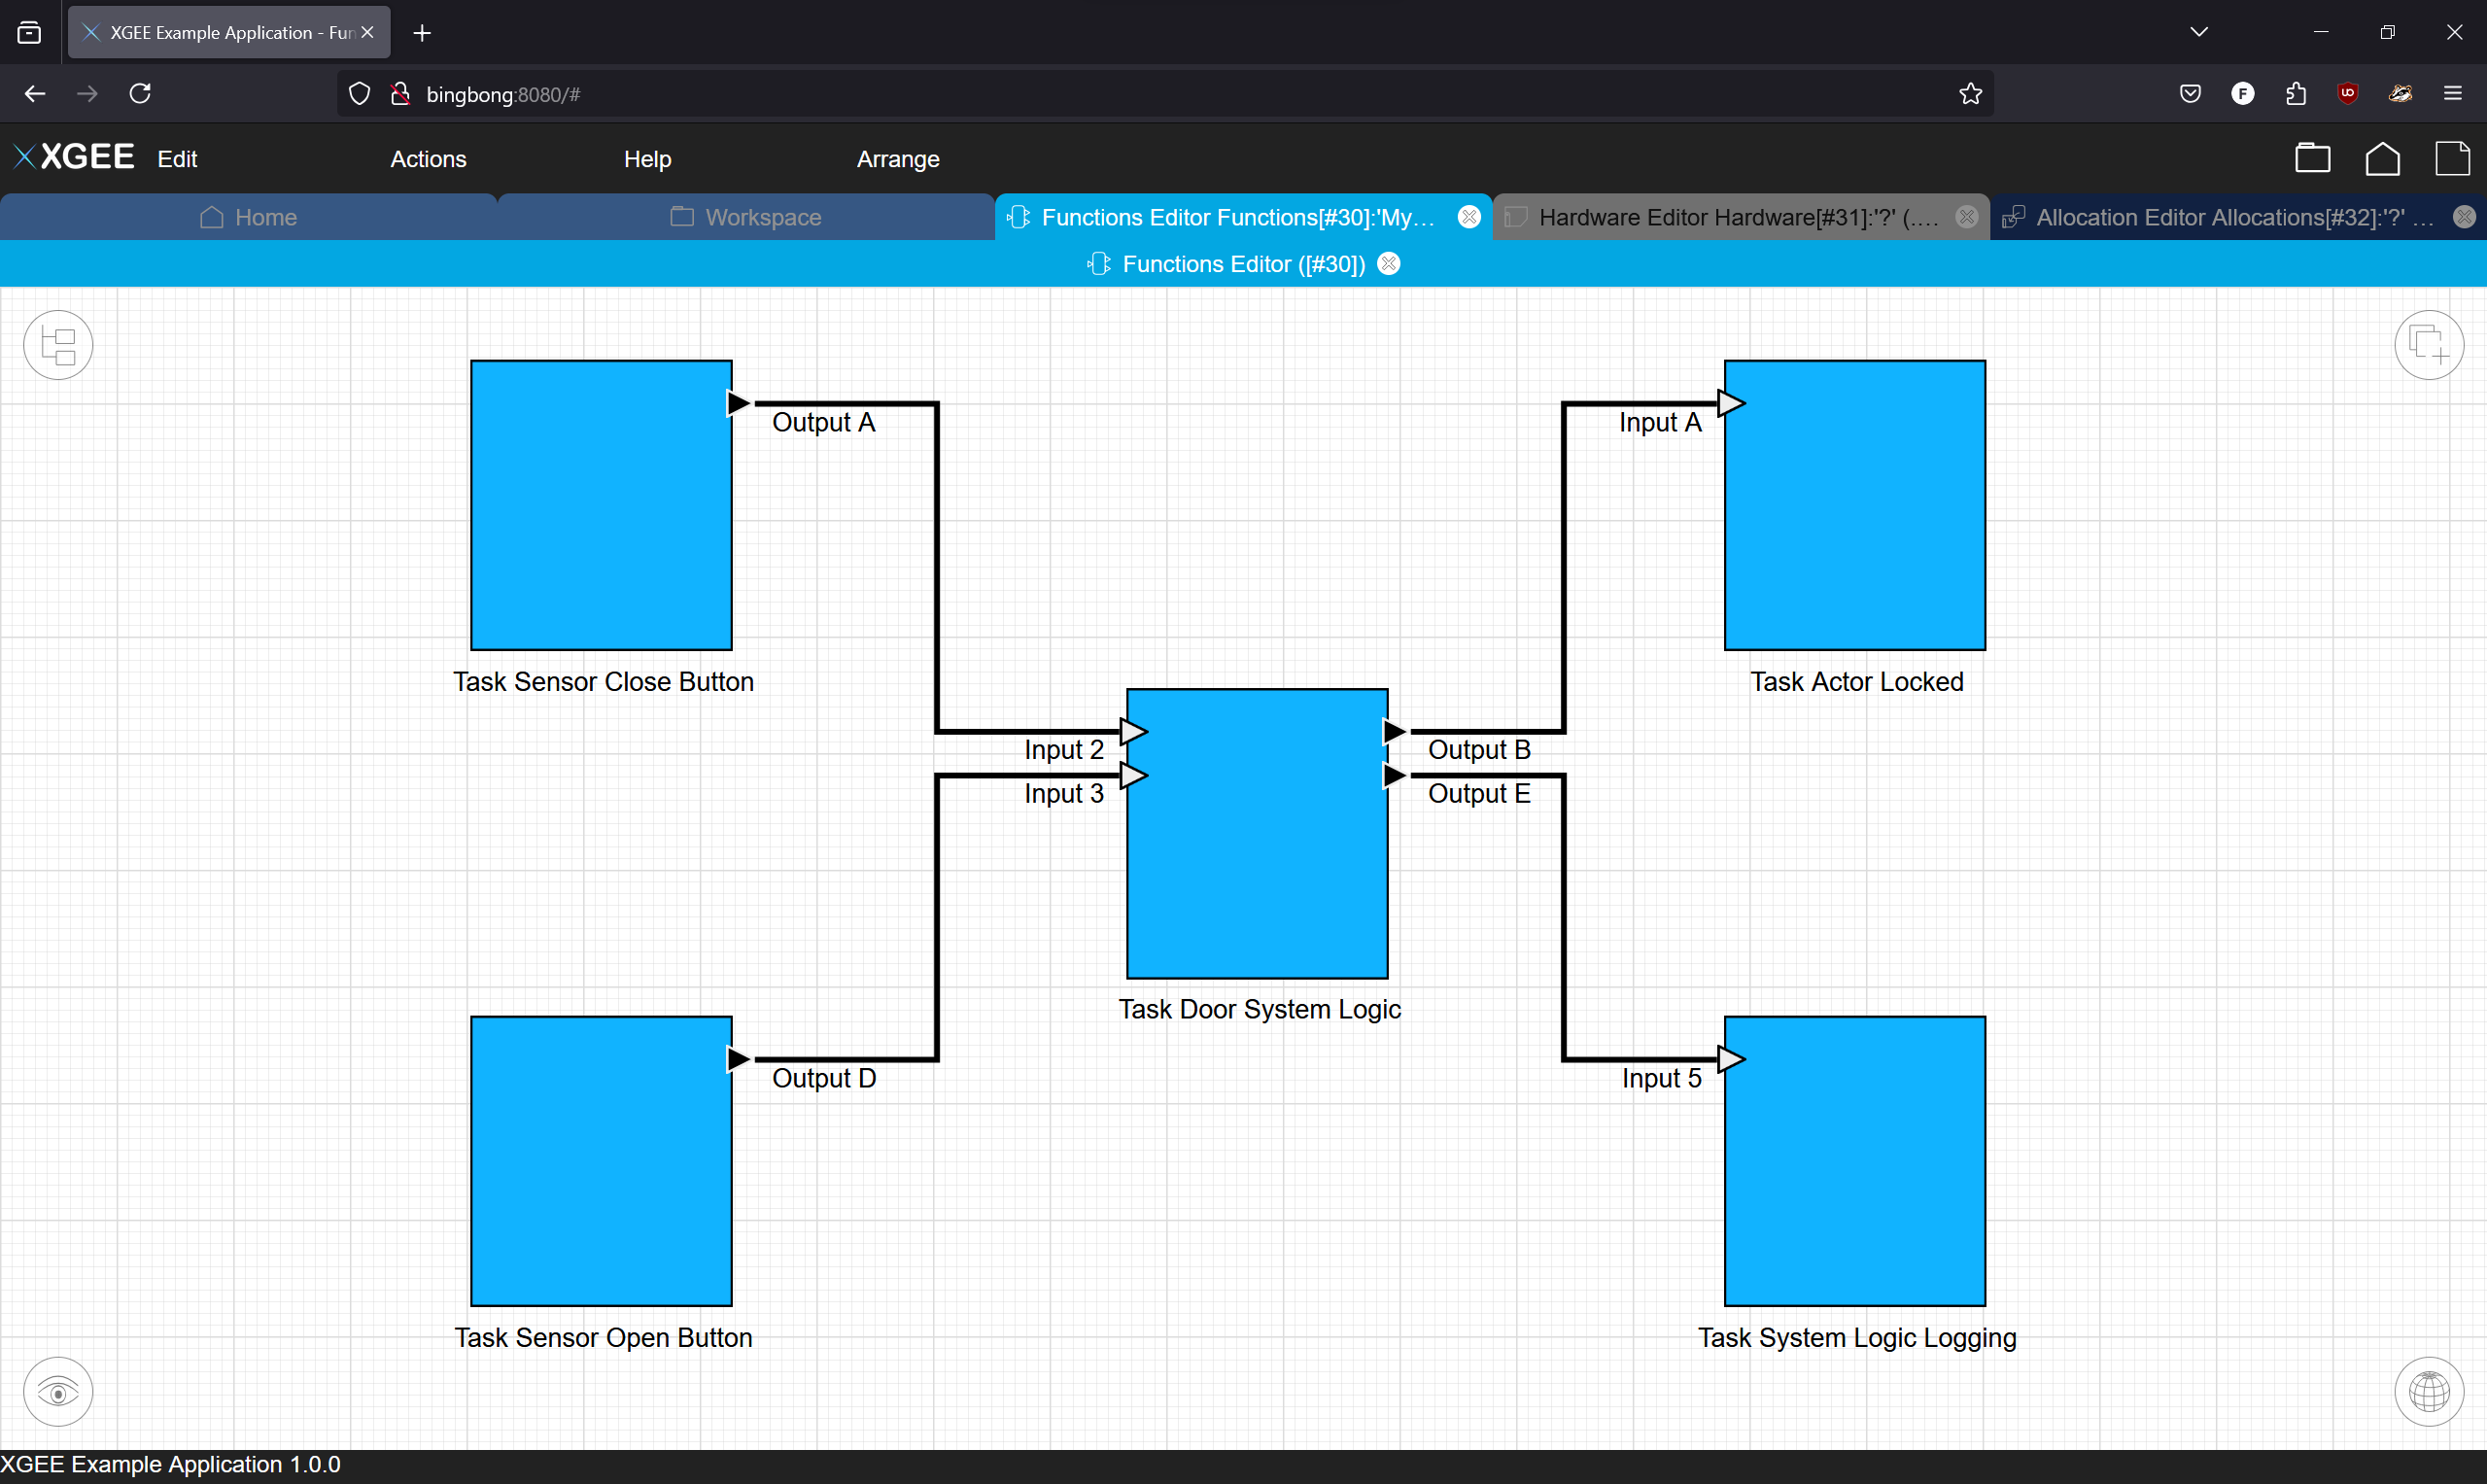
\includegraphics[width=\textwidth]{pictures/functions_unaltered.png}
        \label{fig:functions_unaltered}
    \end{minipage}
    \hfill
    \begin{minipage}{0.4\textwidth}
        \centering
        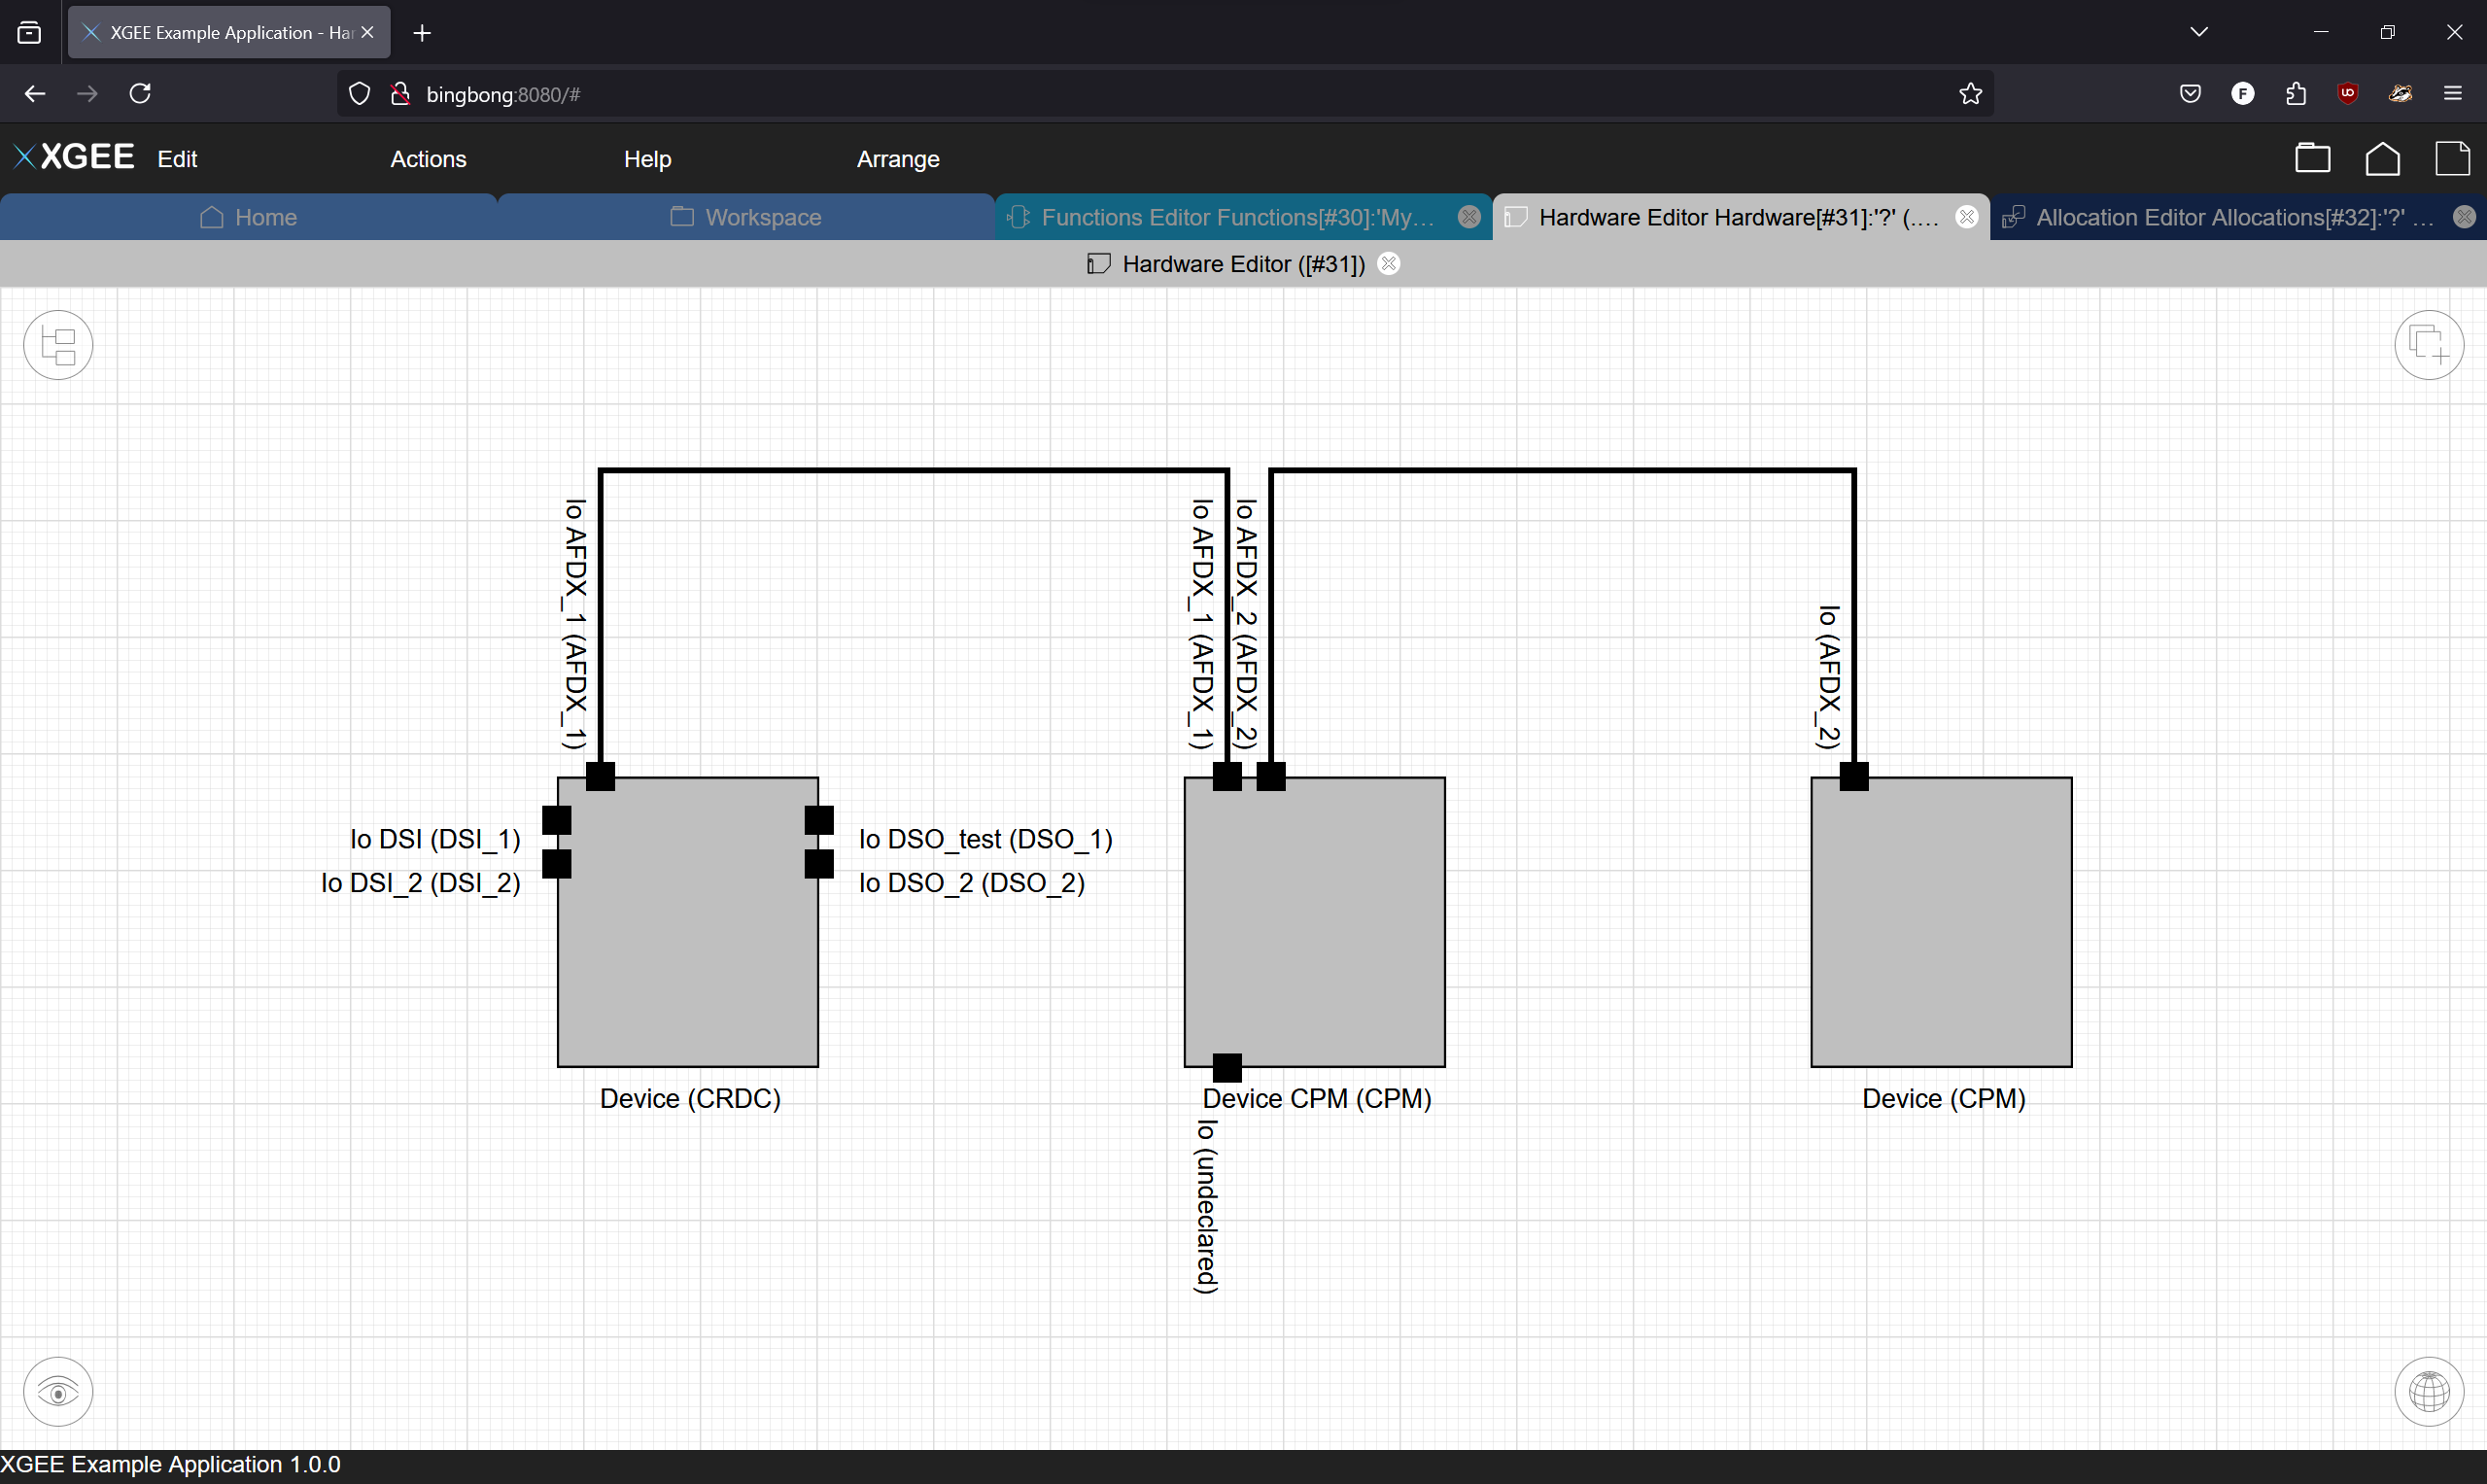
\includegraphics[width=\textwidth]{pictures/hardware_unaltered.png}
        \label{fig:hardware_unaltered}
    \end{minipage}
    \caption[Unaltered models as a basis for testcase generation]{Unaltered models as a basis for testcase generation.\\
    Left: Functions Layer, Right: Hardware Layer}
    \label{fig:unaltered_layers}
\end{figure}
The testcases enumerated in \autoref{tab:test_cases_text} only result in textual error indications. This is because the tested errors can not be detected during the tokenization or syntax steps of the verification pipeline, meaning that visually, the used tokens and their syntax are correct. The errors are only discovered during the comparison or instantiation steps, resulting in only a textual error indication. The first column of the table provides a zoomed-in view of a model containing the error. The second column provides a brief description of the testcase and the indicated textual errors.

\autoref{tab:functional_test_cases_no_errors} contains testcases without any simulated errors to illustrate the pipelines capability to deal with complex models including diverse vertices and intersecting connections. The first colummn provides a brief description, the second and third column provide the visualization within the functions layer and within the hardware layer of the \acrshort{xgee} editor.\\
While the tokenization is functional for three of \acrshort{xgee}s model layers, the allocations layer has not yet been implemented fully into the verification pipeline, meaning that there are currently no meaningful error indications when trying to verify a model in the allocations layer. Hence, the testcases are only shown for the functions and hardware layers.\\
A seperate testcase showcasing the capability of the tokenization pipeline of allocation models can be seen in \autoref{fig:allocations_found_tokens}. All found edges, bounding boxes and their respective token names are overlayed in green on the screenshot of the used model.
\newpage
\begin{longtable}{p{0.2\textwidth} >{\raggedright\arraybackslash}m{0.2\textwidth} >{\raggedright\arraybackslash}m{0.5\textwidth}}
    \caption{Results for test cases with textual and visual error indication.}
    \label{tab:test_cases}\\
    \toprule
    Test Case & Excerpt Visual Error Indication & Textual Error Indication \\
    \midrule
    \endfirsthead
    
    \multicolumn{3}{c}
    {{\bfseries Table \thetable\ continued from previous page}} \\
    \toprule
    Test Case & Excerpt Visual Error Indication & Textual Error Indication \\
    \midrule
    \endhead
    
    \midrule \multicolumn{3}{r}{{Continued on next page}} \\
    \endfoot
    
    \bottomrule
    \endlastfoot
    Functions Layer - Task too Small &  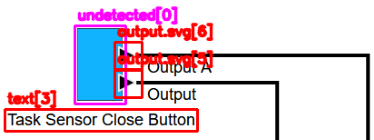
\includegraphics[width=1\linewidth]{pictures/20_task_too_small_output_clip.png} & \textbf{Tokenization}: untokenized pixels. \newline
        \textbf{Syntax}: ['text', 3] is missing a parent element. \newline
        \textbf{Syntax}: ['output.svg', 5] is missing a parent element. \newline
        \textbf{Syntax}: ['output.svg', 6] is missing a parent element. \newline
        \textbf{Instantiation}: output.svg[5] is not instantiated, association cannot connect. \newline
        \textbf{Comparison}: Task Sensor Close Button missing in recognized model. \newline
        \textbf{Comparison}: Signal Door System Logic: B $\rightarrow$ Actor Locked: A missing in recognized model. \newline
        \vdots \\
    \midrule
    Hardware Layer - Device too Small &  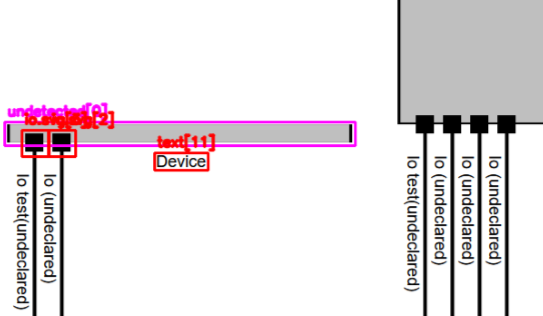
\includegraphics[width=1\linewidth]{pictures/21_device_too_small_output_clip.png} & \textbf{Tokenization}: untokenized pixels. \newline
        \textbf{Syntax}: ['text', 11] is missing a parent element. \newline
        \textbf{Syntax}: ['io.svg', 2] is missing a parent element. \newline
        \textbf{Syntax}: ['io.svg', 3] is missing a parent element. \\
    \midrule
    Functions Layer - Task Wrong Color &  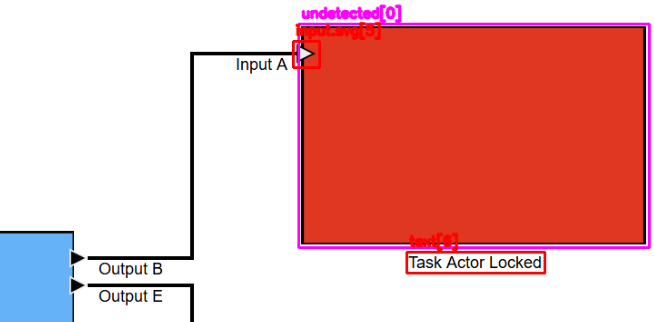
\includegraphics[width=1\linewidth]{pictures/31_wrong_color_task_output_clip.png} & \textbf{Tokenization}: untokenized pixels. \newline
        \textbf{Syntax}: ['text', 6] is missing a parent element. \newline
        \textbf{Syntax}: ['input.svg', 5] is missing a parent element. \newline
        \textbf{Instantiation}: input.svg[5] not instantiated, association cannot connect. \newline
        \textbf{Comparison}: Signal Door System Logic: B $\rightarrow$ Actor Locked: A missing in recognized model. \newline
        \textbf{Comparison}: Signal Door System Logic: E $\rightarrow$ System Logic Logging: 5 missing in recognized model. \newline
        \vdots \\
    \midrule
    Hardware Layer - Device Wrong Color &  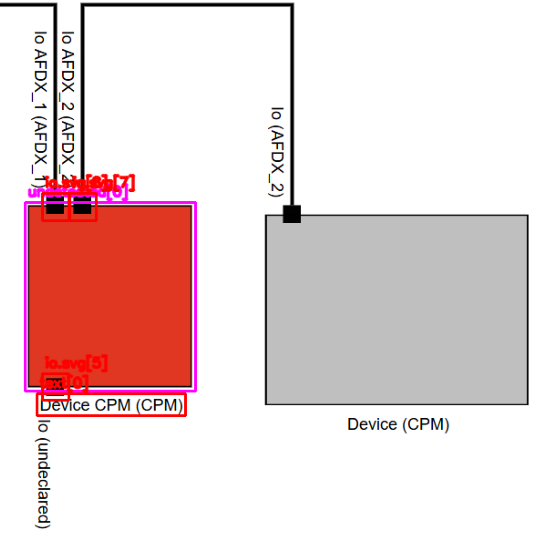
\includegraphics[width=1\linewidth]{pictures/32_wrong_color_task_output_clip.png} & \textbf{Tokenization}: untokenized pixels. \newline
        \textbf{Syntax}: ['text', 10] is missing a parent element. \newline
        \textbf{Syntax}: ['io.svg', 0] is missing a parent element. \newline
        \textbf{Syntax}: ['io.svg', 1] is missing a parent element. \newline
        \vdots \\
    \midrule
    Functions Layer - Free Floating Input & 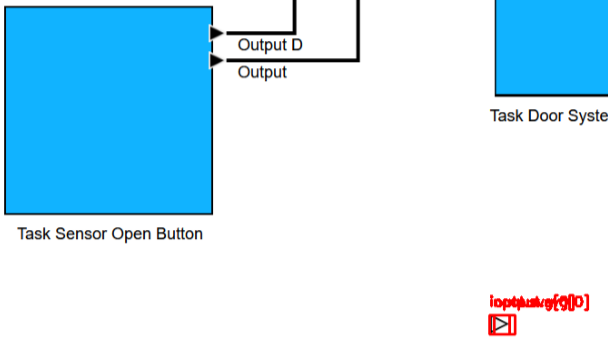
\includegraphics[width=1\linewidth]{pictures/40_free_floating_input_output_clip.png} & \textbf{Syntax}: ['input.svg', 0] is missing a parent element. \newline
        \textbf{Syntax}: ['output.svg', 1] is missing a parent element.\\
    \midrule
    Hardware Layer - Free Floating IO & 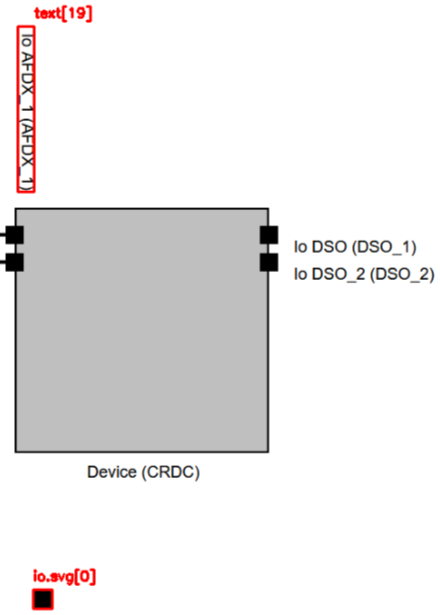
\includegraphics[width=1\linewidth]{pictures/41_free_floating_input_output_clip.png} & \textbf{Syntax}: ['text', 19] is missing a parent element. \newline
        \textbf{Syntax}: ['io.svg', 0] is missing a parent element. \\
    \midrule
    Functions Layer - Free Floating Star & 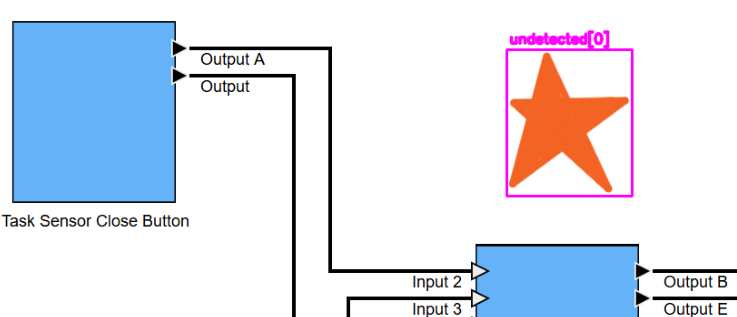
\includegraphics[width=1\linewidth]{pictures/42_free_floating_star_output_clip.png} & \textbf{Tokenization}: untokenized pixels. \\
    \midrule
    Hardware Layer - Free Floating Star & 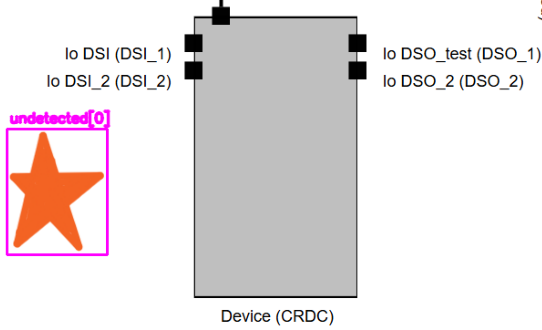
\includegraphics[width=1\linewidth]{pictures/43_free_floating_star_output_clip.png} & \textbf{Tokenization}: untokenized pixels. \\
    \midrule
    Functions Layer - Input Instead of Output & 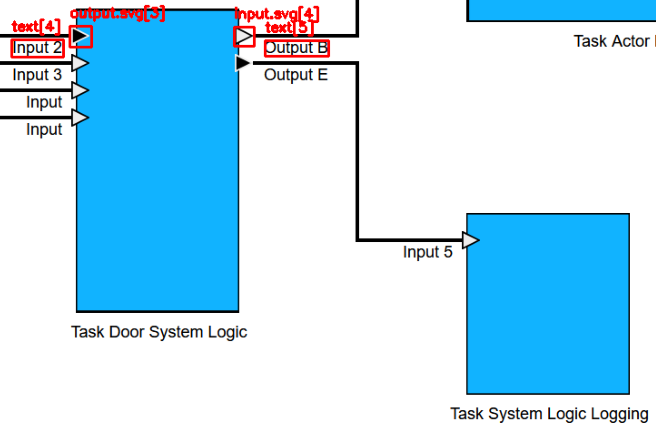
\includegraphics[width=1\linewidth]{pictures/50_input_instead_of_output_output_clip.png} & \textbf{Syntax}: ['text', 4] is missing a parent element. \newline
        \textbf{Syntax}: ['text', 4] is missing a parent element. \newline
        \textbf{Syntax}: ['input.svg', 4] is missing a parent element. \newline
        \textbf{Syntax}: ['output.svg', 3] is missing a parent element. \newline
        \textbf{Instantiation}: Failed to instantiate association. Endpoint input.svg. \newline
        \textbf{Instantiation}: Failed to instantiate association. Endpoint output.svg. \newline
        \textbf{Comparison}: Signal Door System Logic: B $\rightarrow$ Actor Locked: 1 missing. \newline
        \vdots \\
    \midrule
    Functions Layer - Signal Wrong Color & 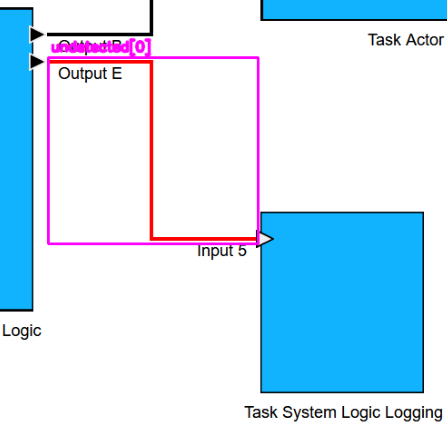
\includegraphics[width=1\linewidth]{pictures/32_signal_wrong_color_output_clip.png} & 
        \textbf{Tokenization}: untokenized pixels. \newline
        \textbf{Syntax}: ['text', 17] is missing a parent element. \newline
        \textbf{Comparison}: Number of Signals in the original model (6) does not match (5). \newline
        \textbf{Comparison}: Signal Door System Logic: E $\rightarrow$ System Logic Logging: 5 missing \\
    \midrule
    Hardware Layer - Signal Wrong Color & 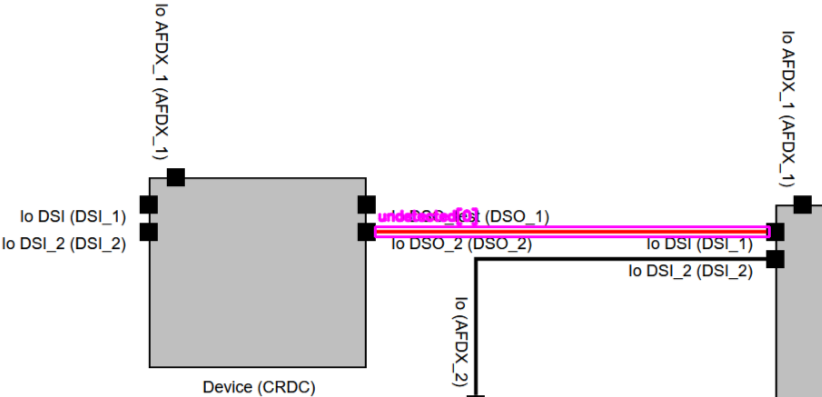
\includegraphics[width=1\linewidth]{pictures/33_signal_wrong_color_output_clip.png} & \textbf{Tokenization}: untokenized pixels. \\
    \midrule
    Functions Layer - Text too Far & 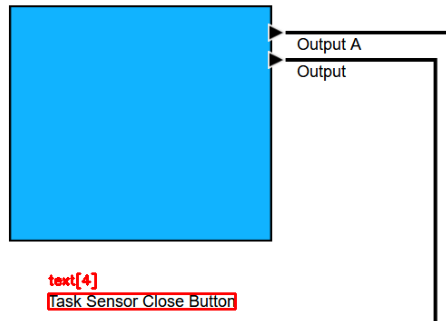
\includegraphics[width=\linewidth]{pictures/60_text_too_far_output_clip.png} & \textbf{Syntax}: ['text', 4] is missing a parent element. \newline
        \textbf{Comparison}: Task "Sensor Close Button" missing in recognized model. \newline
        \textbf{Comparison}: Signal Sensor Close Button: A $\rightarrow$ Door System \\
    \midrule
    Hardware Layer - Text too Near & 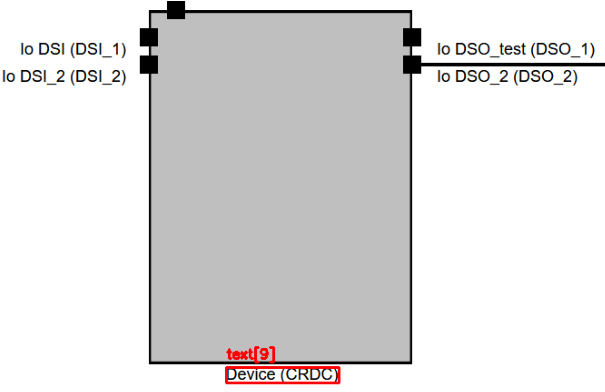
\includegraphics[width=1\linewidth]{pictures/61_text_too_far_output_clip.png} & \textbf{Syntax}:['text', 9] is missing a parent element. \\
\end{longtable}


\begin{longtable}{p{0.2\textwidth} >{\raggedright\arraybackslash}m{0.2\textwidth} >{\raggedright\arraybackslash}m{0.52\textwidth}}
    \caption{Results for test cases with textual error indication.}
    \label{tab:test_cases_text}\\
    \toprule
    Test Case & Excerpt Modified Screenshot & Textual Error Indication \\
    \midrule
    \endfirsthead
    
    \multicolumn{3}{c}{{\bfseries Table \thetable\ continued from previous page}} \\
    \toprule
    Test Case & Excerpt Modified Screenshot & Textual Error Indication \\
    \midrule
    \endhead
    
    \midrule \multicolumn{3}{r}{{Continued on next page}} \\
    \endfoot
    
    \bottomrule
    \endlastfoot
    
    New Task Hiding Other New Task & 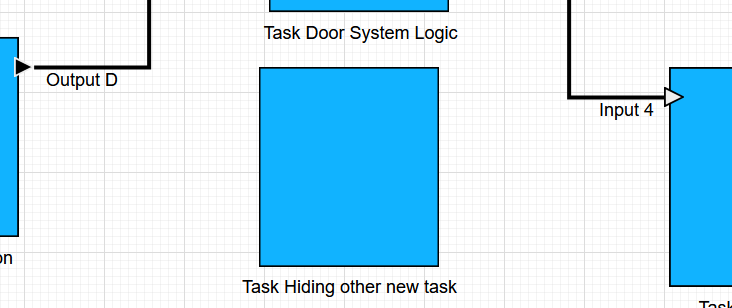
\includegraphics[width=\linewidth]{pictures/61_task_hides_task_input_clip.png} & \textbf{Comparison}: Task Hidden missing \\
    \midrule
    Task Out of Window & 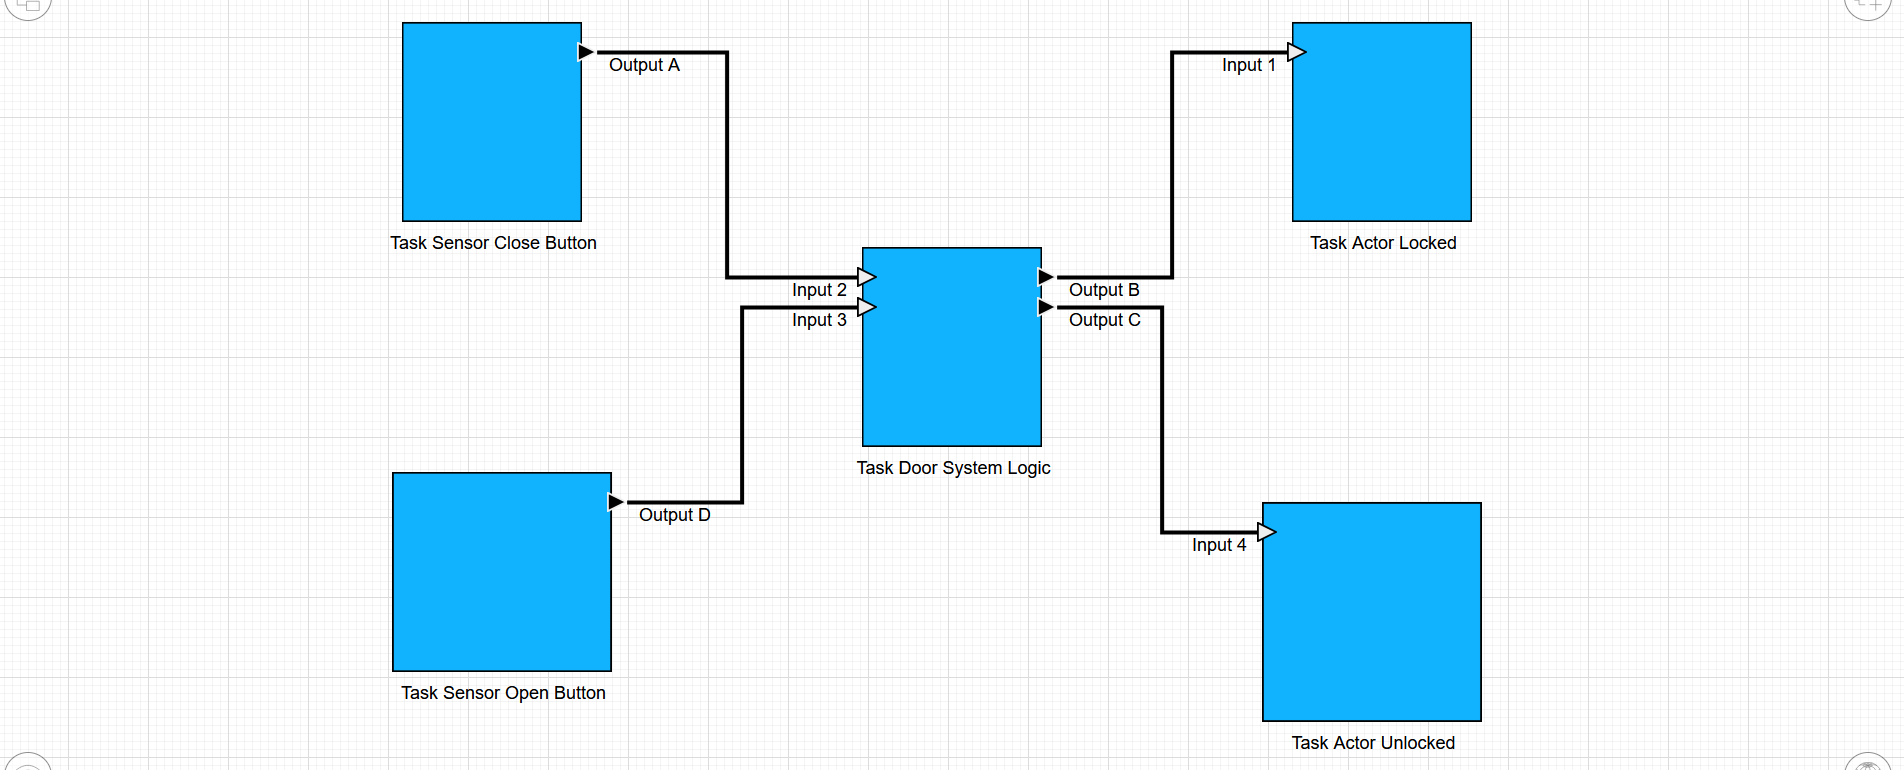
\includegraphics[width=\linewidth]{pictures/63_task_far_away_input_clip.png} & \textbf{Comparison}: Task Far Away missing \\
    \midrule
    Task Deleted in Editor, but Still in Model & 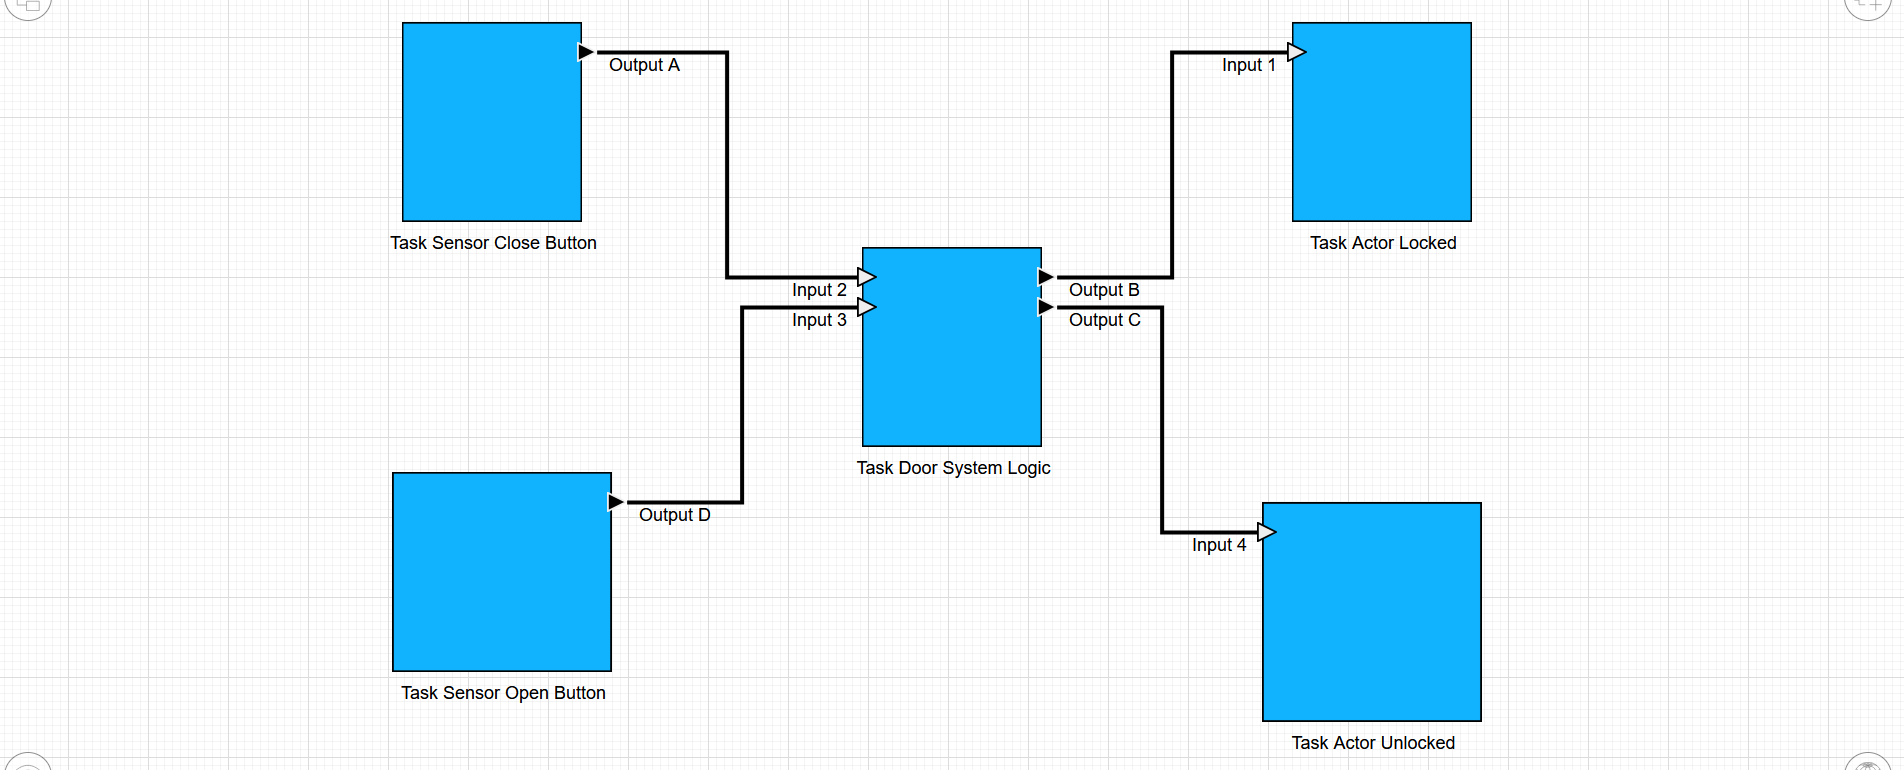
\includegraphics[width=\linewidth]{pictures/63_task_far_away_input_clip.png} & \textbf{Comparison}: Task New Task Already Deleted Missing \\
    \midrule
    Task Created, but Not Yet in Model & \includegraphics[width=\linewidth]{pictures/71_new_task_not_yet_in_model_input_clip.png} & \textbf{Comparison}: Task Newly Created Not Yet in Model Missing in Original Model \\
    \midrule
    Signal Not Connected to Input & \includegraphics[width=\linewidth]{pictures/80_signal_not_connected_to_input_input_clip.png} & \textbf{Comparison}: Signal Door System Logic:C $\rightarrow$ Actor Unlocked:4 Missing \\
    \midrule
    Signal Connected to Wrong Port & \includegraphics[width=\linewidth]{pictures/81_signal_wrong_port_correct_task_input_clip.png} & \textbf{Comparison}: Signal Door System Logic: B $\rightarrow$ Actor Locked: A Missing \newline \textbf{Comparison}: Signal Door System Logic: E $\rightarrow$ System Logic Logging: 5 Missing \\
    \midrule
    Overlapping Intersections & \includegraphics[width=\linewidth]{pictures/92_modified_task_name_input_clip.png} & \textbf{Comparison}: Sensor Open Button:D $\rightarrow$ Door System Logic:3 Missing \newline \textbf{Comparison}: Task Sensor Open Button Missing \\
    \midrule
    Changed Task Name, but Not Yet in Model & \includegraphics[width=\linewidth]{pictures/91_modified_task_name_input_clip.png} & \textbf{Comparison}: Sensor Open Button:D $\rightarrow$ Door System Logic:3 Missing \newline \textbf{Comparison}: Task Sensor Open Button Missing \\
    \midrule
    Encoding Error in Task Name & \includegraphics[width=\linewidth]{pictures/90_encoding_error_input_clip.png} & \textbf{Comparison}: Task Actor Locked Missing \newline \textbf{Comparison}: Signal Door System Logic:B $\rightarrow$ Actor Locked:1 Missing \\
\end{longtable}


\begin{table}[H]
    \caption{Functional Test Cases Demonstrating Correct System Behavior}
    \label{tab:functional_test_cases_no_errors}
    \begin{tabularx}{\textwidth}{@{}>{\hsize=.4\hsize\linewidth=\hsize}X m{0.3\textwidth} m{0.3\textwidth}@{}}
        \toprule
        Test case description & functions layer visualization & hardware layer visualization \\ 
        \midrule
        Processing of vertices with varying sizes and aspect ratios &  
        \includegraphics[width=\linewidth]{pictures/correct_task_size_input_clip.png} & 
        \includegraphics[width=\linewidth]{pictures/correct_task_size_output_clip.png} \\

        \midrule
        Recognition of complex signal intersections in close proximity &  
        \includegraphics[width=\linewidth]{pictures/many_intersections.png} & 
        \includegraphics[width=\linewidth]{pictures/many_intersections_hardware.png} \\

        \midrule
        Function / device has the wrong color - but is still detected by the template matching method. &  
        \includegraphics[width=\linewidth]{pictures/one_in_grey_input_clip.png} & 
        \includegraphics[width=\linewidth]{pictures/one_in_blue_input_clip.png} \\
        \bottomrule
    \end{tabularx}
\end{table}
\chapter{Discussion}
\label{chap:discussion}
This chapter highlights the implemented methods' capability to handle a variety of testcases, as well as current limitations and challenges of the implemented methods, focusing on their impact on error detection, visualization, and overall system efficiency.

\section{Testcases}
As seen in \autoref{chap:evaluation}, all 20 unique testcases are correctly identified and indicated to the user and, as seen in \autoref{tab:functional_test_cases_no_errors}, no errors are reported if none are simulated.\\
In the \textit{free floating star} test case, error detection is straightforward, as the star is detected in the tokenization step and highlighted. In the \textit{input instead of output} and \textit{free floating input / \acrshort{io}} testcases, all vertices are known, but they are not correctly positioned, resulting in an error indication during the syntax step of the pipeline. Similar error indications are generated in the \textit{text too far} and \textit{text too near} test cases, because they too are correctly identified during tokenization but have a slightly shifted position, resulting in syntax errors.

\begin{wrapfigure}{r}{0.4\textwidth}
    \centering
    \includegraphics[width=0.4\textwidth]{pictures/allocations_thin_edges.png}
    \caption{Example of the thin edges in the allocations editor, which are hard to detect using the currend edge detection method.}
    \label{fig:allocations_thin_edges}
\end{wrapfigure}
In \textit{device wrong color}, \textit{task wrong color} and \textit{signal wrong color}, the color of one of the vertices or edges is changed such, that it is no longer being detected in the tokenization step. This results in untokenized pixels, as well as a number of additional errors, because for example, the associated \acrshort{io} ports of the changed device are now seemingly floating in space, resulting in wrong syntax. The same problem arises in the simulated testcases \textit{task / device too small}.

Further problems arise when instantiating and comparing the new model without the changed device. These additional errors are reported, making it harder for the user to identify the original problem cause.\\
Furthermore, as illustrated in \autoref{tab:functional_test_cases_no_errors}, a changed color is only reported as an error, if the intensity of the original and altered color is significantly different. This is because \acrshort{opencv}'s \textit{matchtemplate} function compares the pixels intensities, effectively ignoring colors. This could be improved by running the template matching algorithm seperately for each color channel and then comparing the results or by incorporating a different method more suitable for differentiating color hues.

\section{Limitations of current Methods}
The current implementation is, in large parts, model driven, meaning it can recognize the current model and query it for information, such as a list of the used token types and the location of their respective \textit{.svg} files.\\
However, a current limitation is the amount of information that can be queried and utilized. For instance, the current implementation does not query the current model layer, making it difficult to differentiate between \textit{function}-, \textit{hardware}-, and \textit{allocation} layers. This can lead to less efficient tokenization. For example, during text recognition, the image is searched for rotated text, regardless of whether the current model contains any.\\
Another limitation lies in the template matching method. As stated in \autoref{chap:new_concepts}, the current implementation applies each template to the image, which works well if the used templates are stored within the model, enabling the system to query them and dynamically choose the correct templates for each model layer. However, for edge and intersection detection, no such convenient template files are stored. Instead, the templates are generated with a fixed size, making it harder to adapt the system to changes in edge width, color, or intersection visualizations.\\
Another limitation stems from the both the visualization and the edge detection pipeline's difficulty in identifying the edges connecting subtasks within the allocations editor (see \autoref{fig:allocations_thin_edges}). This is because these edges are too thin and lack sufficient contrast for accurate detection. Implementing a more robust algorithm or designing a visualization that is easier to detect for computer vision algorithms could enhance the detection process, potentially allowing it to be integrated into the edge detection pipeline.\\
Another limiting factor is the lack of error handling mechanisms. If an error occurs during the verification, it can disrupt or stop the entire workflow. Furthermore, a single error can result in many error indications, as discussed in \autoref{chap:discussion}, hampering the user's ability to quickly find the root cause of the error indications.

All of these limitations could be addressed by enhancing the current implementation with additional features, such as querying the model for more information, dynamically generating templates, or implementing more robust error handling mechanisms.\\


\chapter{Outlook}
\label{chap:outlook}
This chapter explores potential improvements and future directions for the methods and tools introduced in this thesis, with a focus on insights gained from the analysis of test cases. While the proposed edge, vertex, and text detection algorithms perform reliably in most scenarios, certain limitations became evident when applied to complex or ambiguous test cases.

\section{Edge Detection Further Improvements}
\label{sec:edge_detection_further_improvements}
The method introduced in this thesis successfully detects and processes nearly all edges within \acrshort{xgee}. In contrast to the previous algorithm, it can identify edges in any orientation, regardless of their start or endpoint or order of their line segments. Furthermore, it is capable of processing and interpreting intersections and signal containers, making it well-suited for handling large, complex models. The method performs reliably across all three editor models, provided the models are formatted correctly (the zoom level has to be set to 100\% across the entire operating system for the edge detection to work reliably). In cases where multiple edges overlap or many intersections are within a few pixels of each other, an error is reported, as the method, as well as human operators, can not reliably interpret the image. This enforces an unambiguous model layout, which is achieved by either an automatic arrangement algorithm or the user.

The current intersection detection relies on a very specific visualization, where intersecting lines simply cross. This poses a limitation, as the method cannot adapt if the intersection visualization changes, for instance, to better display the intersection of multiple edges. A potential solution to this problem could involve extracting the intersection graphic from the screenshot by predicting the intersection's position based on the detected edges. This approach would enable the method to adapt to different intersection visualizations, as long as the edges remain detectable.

A notable problem arises when vertices with surrounding black edges, such as devices or functions, are scaled sufficiently, making their edges resemble signal-carrying edges (see \autoref  {tab:functional_test_cases_no_errors}). This complicates their differentiation. In this case, a possible solution would be to let the vertex detection run first and exclude the found areas when applying the edge detection. Alternatively, the presence of colored pixels around the edges could be checked more thoroughly, as the background around edges is typically white, unlike the areas inside device or function vertices. This way, any obstructions caused by the vertices can be avoided.\\
Another issue may arise if the edges are configured by the user in an unexpected way. For instance, an intersection hidden behind vertices or signal containers cannot be properly interpreted by the current method, which could lead to unexpected results. Future improvements to the \acrshort{xgee} editor, such as a more advanced automatic arrangement algorithm, could reduce or eliminate the risk of ambiguous user input that would result in such cases. Another potential solution would be to search for edges along the sides of detected devices and functions and attempt to connect them. However, this approach might fail if multiple edges run behind a single device or function, which would also make the visualization difficult for a human user to interpret.

Another issue arises from edges connecting subtasks within the allocations editor. They often overlap with text, are too thin, and have too little contrast to be detected accurately. In a future version of \acrshort{xgee}'s visualization, enhancing the readability of subtask edges would enable a computer vision algorithm to detect them reliably, enabeling useful user feedback and thus improving the verification tool.

\section{Vertex Detection Further Improvements}
\label{sec:vertex_detection_further_improvements}
The proposed method can reliably detect almost all vertices across all of \acrshort{xgee}'s model layers, regardless of their dimensions or placement. It can effectively distinguish between subvertices and main vertices by querying the model and applying the appropriate template matching algorithm based on the properties of each template. Additionally, the current editor model is queried to identify the set of utilized vertices, which are subsequently detected. This adaptability enhances both the efficiency and reliability of the method, enabling it to handle changes in the model.\\
As described in \autoref{chap:new_concepts}, the current method identifies each token type within the allocation layer by following a structured detection sequence. First, subtasks are identified and subsequently erased from the screenshot to prevent interference with the detection of underlying vertices.\\
Currently, this approach is only used to enable the detection of devices in the allocations layer. In the future, extending this approach across the entire tokenization pipeline could significantly enhance vertex detection, ensuring that no vertices are obscured, no vertex is detected multiple times, and similar vertices, edges, or text are not mistakenly identified as one another.\\
To implement this improvement, the following steps could be taken:

\begin{itemize}
    \item Process all vertices, edges and text in hierarchical top-down order, starting with subvertices and ending with the main vertices, followed by text and edges.
    \item Query the parent vertex's main color and use it to erase all found vertices.
    \item Dynamically update the input image after each iteration and pass it to the next step in the tokenization pipeline.
    \item Correctly handle cases where subvertices, such as \acrshort{io} ports, only partially overlap with their parent vertices.
\end{itemize}

This approach would systematically simplify the screenshot with each step of the tokenization pipeline, effectively only leaving the untokenized pixels on a white background in the end. After the vertex detection step, the remaining pixels would be passed to the text detection algorithm, which would then identify any remaining text. Finally, the edge detection algorithm would process the remaining pixels, detecting any edges without the possibility of interference from other vertices. This approach would, however, require a way to deal with overlapping text labels, as they would most likely be partially removed in previous steps, making it impossible to properly recognize them.\\

Another possible improvement could be made by enabeling the current method to detect subvertices of subtasks (very small inputs and outputs, as seen in \autoref{fig:allocations_thin_edges}), which are currently excluded from detection due to their small size. These \textit{subsubvertices} are challenging to differentiate from noise, character fragments, or edge segments using \acrshort{opencv}'s built in methods. Employing image preprocessing techniques or refining or exchanging the template matching method could improve the detection of these smaller elements and thus enable a more precise visualization verification.

\section{Text Detection Future Improvements}
\label{sec:text_detection_future_improvements}
Currently, the text recognition system can detect almost any text present within \acrshort{xgee}. Regardless of the current editor, the screenshot is rotated and analyzed to identify any rotated text, which contributes to text detection being the most time consuming component of the visualization verification process.

Optimizing the performance of the text detection algorithm would significantly reduce the overall processing time. This could be achieved by identifying the specific editor type to allow the system to selectively search for rotated characters only when they are expected to be present in the image. Additionally, running the visualization verification on a \acrshort{gpu}, parallelizing the text detection to run simultaneous to the edge- and vertex detection or using a more traditional text detection algorithm which does not require as much computational power as Easy\acrshort{ocr} would enable the system to process larger models more quickly and efficiently, addressing the current bottleneck in the pipeline.\\
Currently, the average runtime of the verification pipeline on an Intel Core Ultra 9 185H \acrshort{cpu} is 54 seconds, with 76\% of runtime spent on character recognition.\\
A new \acrshort{ocr} model would also potentially allow for a more precise way to filter out falsely read characters instead of removing every recognized word shorter than three letters.

Another potential improvement could be made regarding the text recognition's accuracy. Currently, the method is limited by the quality of the input image and the Easy\acrshort{ocr} library. This is because most \acrshort{ocr} engines are trained on books, where text is orderly structured and has a predictable orientation. In contrast, the text in \acrshort{xgee} models is often rotated, distorted, or partially occluded, making it difficult for the \acrshort{ocr} engine to recognize. Additionally, individual numbers are hard for Easy\acrshort{ocr} to detect reliably.\\
Training a custom \acrshort{ocr} model on a dataset of \acrshort{xgee} text images could improve the recognition accuracy, as the model would be specifically tailored to the unique characteristics of \acrshort{xgee} text. In future implementations, this could be achieved by automatically generating the training data alongside the correct text by directly querying the model.\\
A simpler way to solve the problem of wrongly detected characters could be improved error handeling, to indicate these types of errors to the user in a simple and clean way. This would enable the user to quickly identify and correct any false errors, reducing the time spent on verification.

\section{Expanding to other Domains or Applications}
\label{sec:expanding_to_other_domains}
As described in \autoref{chap:evaluation}, the current implementation is optimized to work model driven in the functions- and hardware layer. Further working on the implementation into the allocations layer would be a logical next step, fully enabeling the verification tool to work with all three of \acrshort{xgee}'s editors, dynamically changing with the model. However, because of the higher complexity of the allocations layer, this would require restructuring the current implementation to consider the order of detection and the hierarchical structure of the model in all steps of the verification pipeline.

One of the goals of this thesis was to generalize the used tokenization algorithms to work in all three of \acrshort{xgee}'s editors. Expanding upon this idea, a future verification pipeline could be able to understand a wide range of different editors, potentially enabeling the verification of editors completely seperated from the verification program. This could be achieved by implementing a more general tokenization pipeline, which could be configured to work with any editor, given the correct templates and cofiguration files.\\
Enabeling the verification to work with editor models like Simulink and other widely used modeling tools would make the verification tool more versatile and useful to a wide audience, potentially resulting in an increase in demand for automatic visualization verification tools.

\normalem
\nocite{*}
\printbibliography[heading=bibintoc,title=Bibliography]

\appendix
\pretocmd{\chapter}{
	\cleardoublepage
	\pagenumbering{arabic}
	\renewcommand*{\thepage}{\thechapter\arabic{page}}
}{}{}
\end{sloppypar}
\end{document}